% \begin{center}
%   \centering
%   \noindent
%   \textit{If I could remember the names of all these particles, I'd be a botanist.} --- Enrico Fermi
% \end{center}

\chapter{The Standard Model of Particle Physics}
\label{sec:01_sm}

\begin{center}
	\centering
	\noindent
	\textit{Before I came here, I was confused about this subject. Having listened to your lecture, I am still confused. But on a higher level.} --- Enrico Fermi\footnote{Also an accurate representation of my understanding of the SM before and after my PhD.}
\end{center}


\begin{figure}
	\centering
	\captionsetup{justification=centering}
	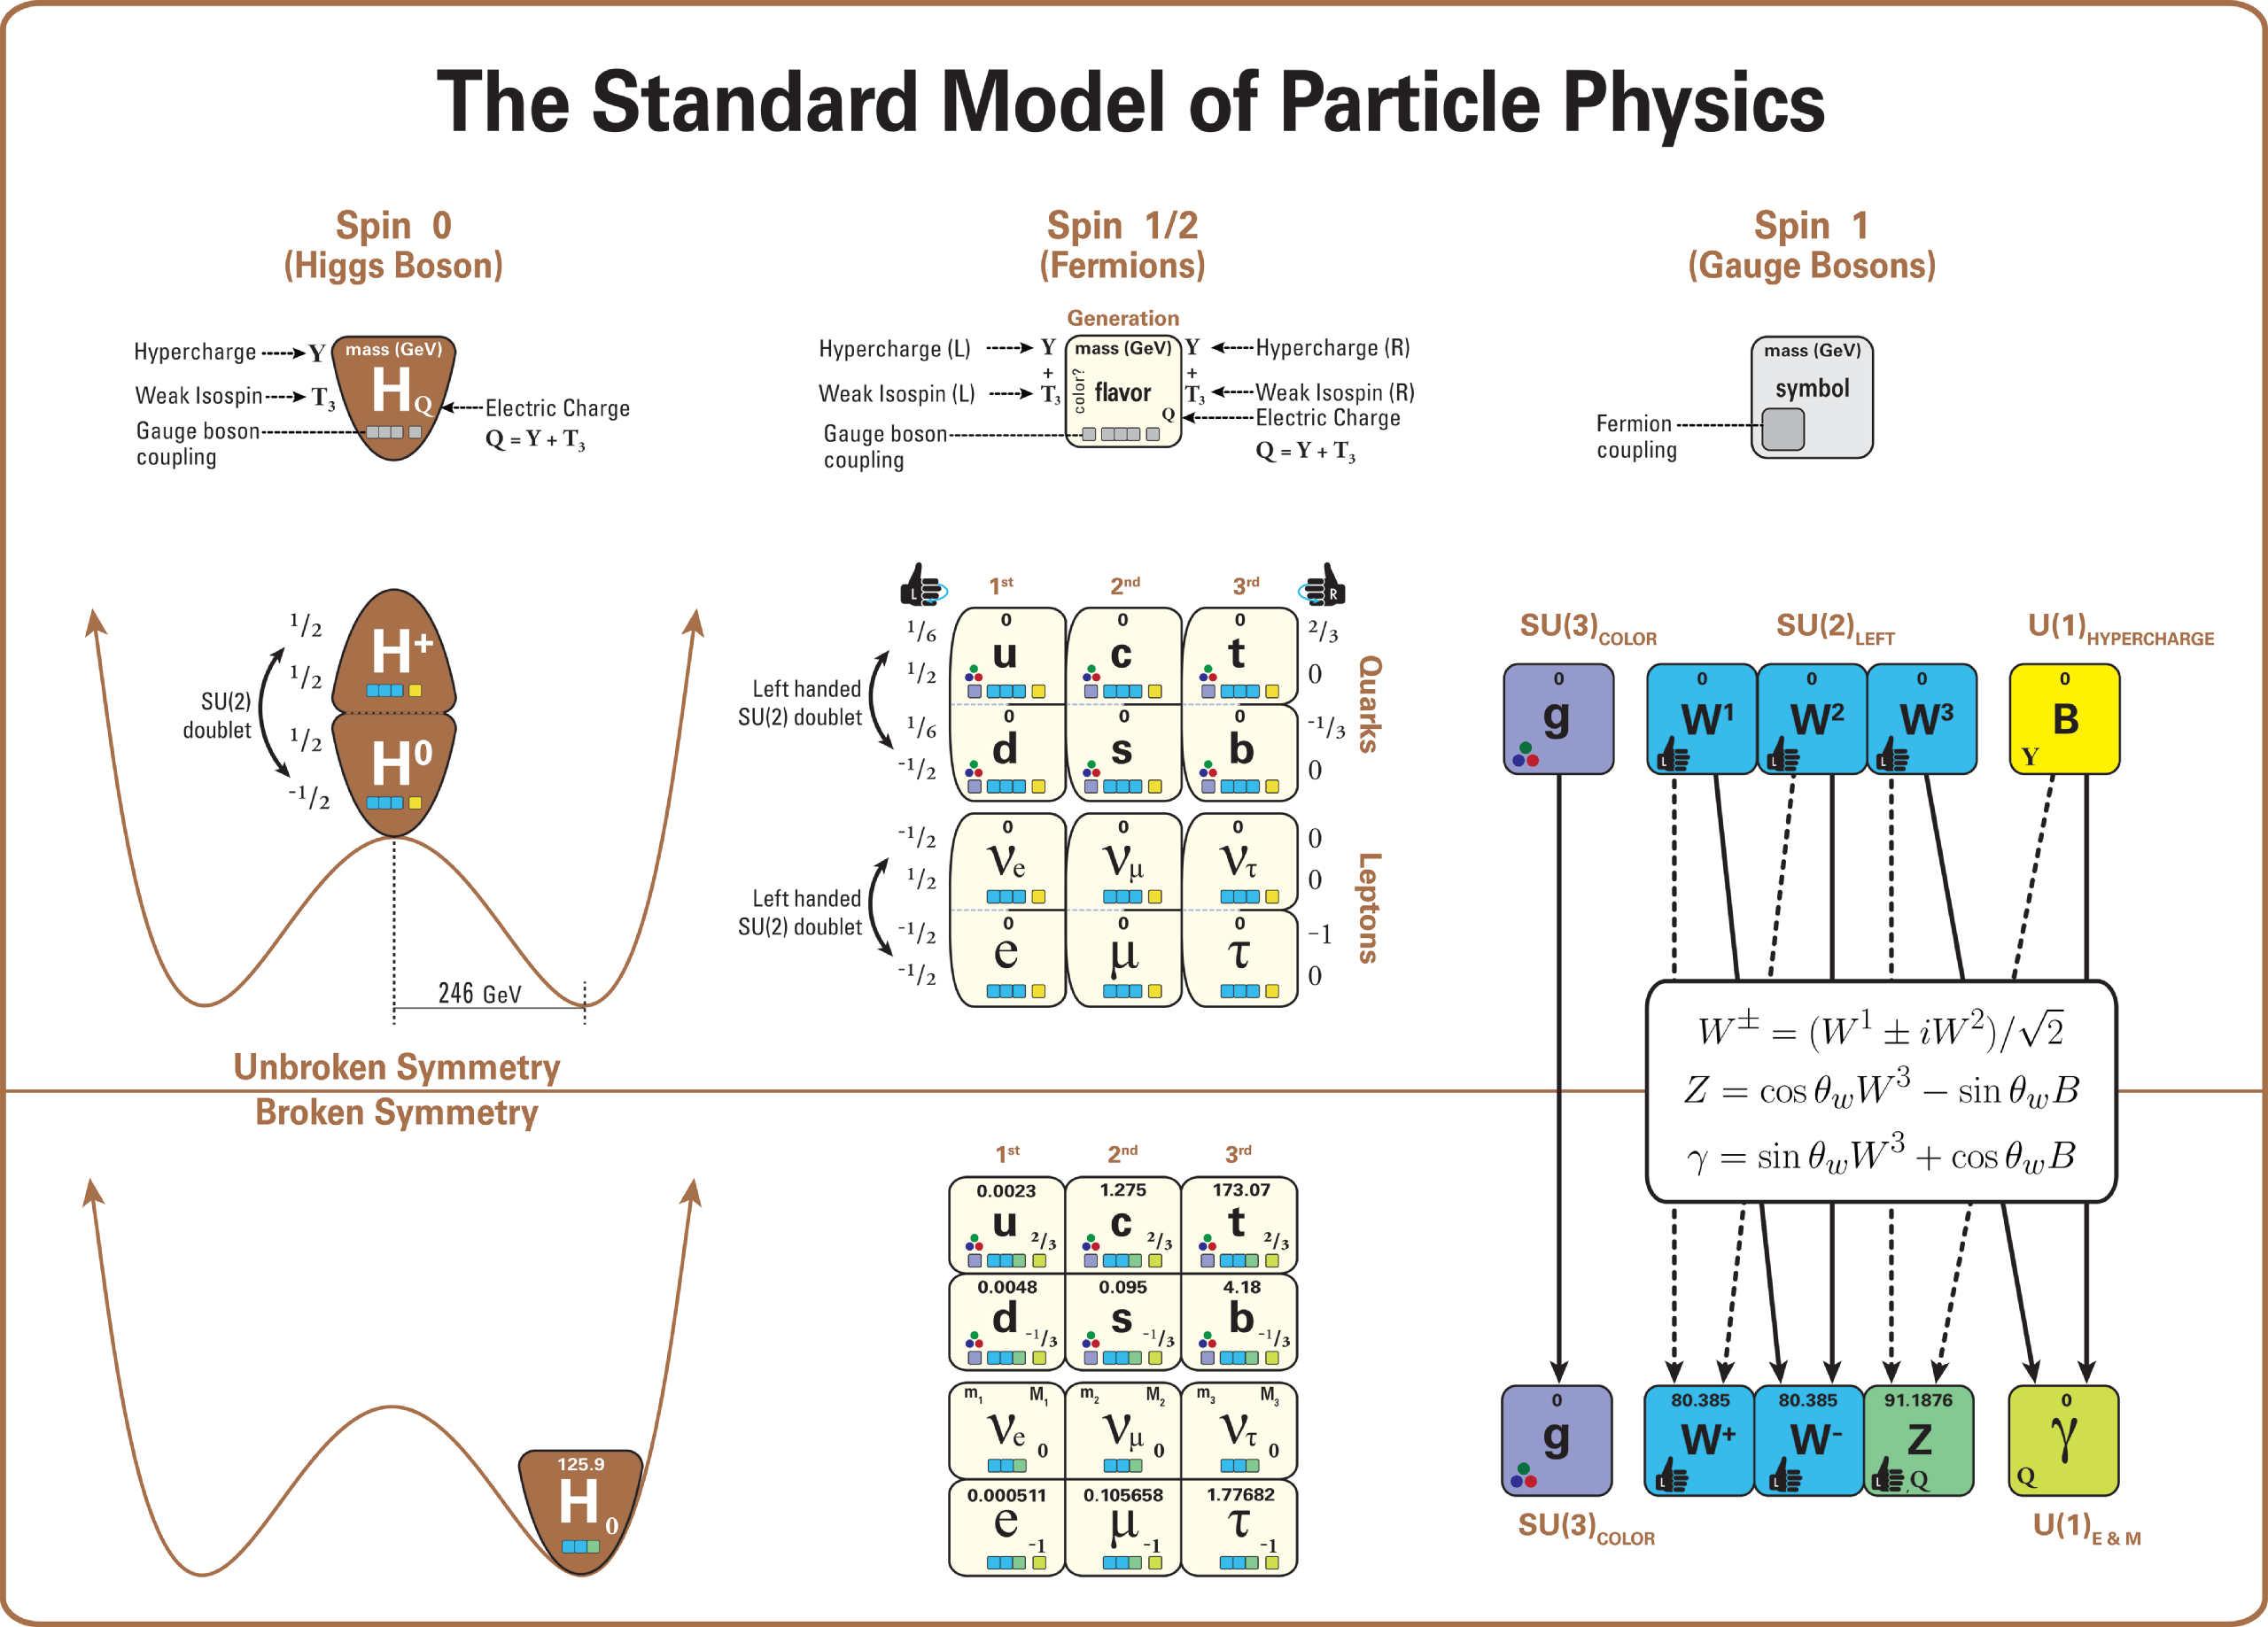
\includegraphics[width=\textwidth]{figures/01-SM-03-SM/Standard_Model_Of_Particle_Physics--Most_Complete_Diagram.png}
	\caption{A graphical summary of the SM, reproduced from Ref.~\cite{SMMostCompleteDiagram}.}
	\label{fig:01_sm_summary}
\end{figure}

We are now ready to describe the standard model (SM)!
It is a renormalizable, quantum Yang-Mills theory, and is illustrated nicely in Figure~\ref{fig:01_sm_summary}.
Before electroweak symmetry breaking (EWSB) --- a form of spontaneous symmetry breaking (SSB) --- it possessed the gauge symmetry $\SU[3]_{\mathrm{C}} \times \SU[2]_{\mathrm{L}} \times \UU[1]_{\mathrm{Y}}$, with $C$, $L$, and $Y$ standing for color, left, and hypercharge, respectively.
%  (their significance will be explained in the following sections).
These three groups correspond to the strong, weak, and electromagnetic forces, with eight, three, and one generators or gauge bosons, respectively.
The relative strengths of each interaction, as well as gravity's, are shown in Table~\ref{tab:01_sm_coupling_constants}, based on the equivalent of the fine structure constant of each force, $\alpha_f = \cnicefrac{g_f}{4\pi}$, where $g_f$ is the respective coupling constant.

The SM contains six fermions charged and uncharged under the $\SU[3]_{\mathrm{C}}$ symmetry each, called the ``quarks'' and ``leptons'', respectively.
% --- the ``quarks'' --- and six fermions uncharged --- the ``leptons''.
The left-handed fermions live as pairs in $\SU[2]_{\mathrm{L}}$ doublets, while the right-handed fermions in singlets.
The six types of fermions are referred to as different ``flavors'', grouped into three generations as in Figure~\ref{fig:01_sm_summary}.

The SM also contains a complex scalar $\SU[2]_{\mathrm{Y}}$-doublet called the Higgs field, which is associated with EWSB.
As shown in Figure~\ref{fig:01_sm_summary}, it initially is at the center of a ``sombrero'' potential because of which, before EWSB, the gauge bosons, fermions, and the Higgs field are all massless.

% where the subscripts will be explained in the following sections, with massless gauge bosons and fermions a zero vacuum expectation value (VEV) for the Higgs field.
EWSB is hypothesized to have occurred during the electroweak epoch (see Figure~\ref{fig:00_timeline}), where the $\SU[2]_{\mathrm{L}} \times \UU[1]_{\mathrm{Y}}$ global symmetry broke to the $\UU[1]_{\mathrm{EM}}$ of QED.
Through this, the Higgs field obtained a non-zero vacuum expectation value (VEV), imbuing all the fermions, three of the gauge bosons, and the Higgs boson with mass --- a process referred to as the Higgs mechanism.
The outcome is the state of the universe and physics as we know it.

Of course, as outlined in the introduction, this picture does not explain myriad phenomena in fundamental physics, including dark matter, dark energy, baryon asymmetry, and neutrino masses.
This is why it is crucial to test the SM as rigorously and in as broad a phase space as possible, in order to identify any cracks that may point to new physics.

% The relative strength of each of their interactions is typically quantified by the equivalent of the fine structure constant for each force, $\alpha_f = \cnicefrac{g_f}{4\pi}$, where $g_f$ is the coupling constant.
% This is shown in Table~\ref{tab:01_sm_coupling_constants} for each force, as well as gravity for illustrative purposes.

\begin{table}[htbp]
    \centering
	\caption{Approximate magnitude of the strengths of the four fundamental forces at an energy scale of around 100\MeV.}
	\renewcommand{\arraystretch}{1.5}
    \begin{tabular}{ll}
        \toprule
        \textbf{Force} & \textbf{Strength}\\
        \midrule
        Electromagnetic &
        $\alpha_{\mathrm{EM}} \approx \frac{1}{137}$ \\
        Weak &
        $\alpha_W \approx \frac{1}{30}$\\
        Strong &
        $\alpha_s \approx 1$\\
        Gravity &
        $\alpha_G  \approx 10^{-38}$\\
        \cbottomrule
    \end{tabular}
	\label{tab:01_sm_coupling_constants}
\end{table}

In this chapter, we will briefly walk through different areas of the SM.
Having discussed QED in Chapter~\ref{sec:01_qft_gt}, we begin with the remaining two fundamental interactions: quantum chromodynamics (Section~\ref{sec:01_sm_qcd}); and weak interactions and electroweak unification (Section~\ref{sec:01_sm_ew}).
% As we will see, the phenomenology of these forces is dictated by the ``running'' of their coupling constants; i.e., the dependence of the strength of the interactions on the energy scale at which they are probed, plotted in Figure~\ref{fig:01_sm_running}.
Finally, in Section~\ref{sec:01_higgs}, we will discuss the Higgs sector and pair production of the Higgs boson, which is the focus of this dissertation.


\section{Quantum chromodynamics}
\label{sec:01_sm_qcd}

Quantum chromodynamics (QCD) is a quantum Yang-Mills field theory describing the strong force, with the gauge group $\SU[3]$.
$\SU[3]$ has eight generators and, hence, eight gauge bosons ($G_\mu$) called gluons.
The only other elementary particles which interact with the strong force --- i.e., which don't live in the trivial representation of $\SU[3]$ --- are the quarks.
They live in the three-dimensional fundamental representation and thus possess three extra DoFs beyond vanilla spinors, which we call their ``color'' (hence, quantum \textit{chromo}dynamics).
The three orthogonal eigenstates in this representation are colloquially referred to as labeled red, green, and blue, and mathematically the quark fields ($q_\alpha$) labeled with extra color indices $i = 1, 2, 3$.

Putting this together, the QCD Lagrangian, with all the indices labeled explicitly is:
\begin{equation}
	\label{eq:01_sm_qcd_lagrangian}
	\mathcal L = -\frac{1}{4} G^a_{\mu\nu} G^{a\mu\nu} + \sum_{f = 1}^6 \bar q_{\alpha f i} [\delta_{ij}(i\cslashed \partial_{\alpha\beta} - m \delta_{\alpha\beta}) + g_s \cslashed G^a_{\alpha\beta} t_{ij}^a] q_{\beta f j}
\end{equation}
where $g_s$ is the strong coupling constant, $G^a_{\mu\nu} = \partial_\mu G^a_\nu - \partial_\nu G^a_\mu + g_s f^{abc} G^b_\mu G^c_\nu$ is the gluon field strength tensor, $f^{abc}$ are the structure constants of $\SU[3]$, $t^a$ are the generators of $\SU[3]$ in the fundamental representation, the sum over $f$ is running over the six flavors, and the indices $a$ and $i, j$ label the eight gluons and the three colors of quarks, respectively.
The six flavors of quarks have different masses and charges, as shown in Figure~\ref{fig:01_sm_qcd_quarks}.

\begin{figure}[ht]
	\centering
	\captionsetup{justification=centering}
	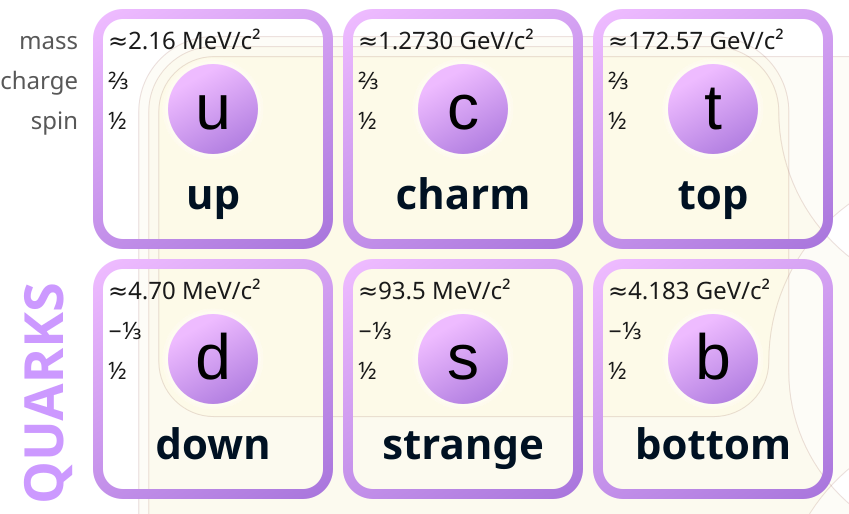
\includegraphics[width=0.5\textwidth]{figures/01-SM-03-SM/qcd/quarks.png}
	\caption{The quarks in the SM, reproduced from Ref.~\cite{enwiki:1238968997}.}
	\label{fig:01_sm_qcd_quarks}
\end{figure}

QCD is an extremely rich and complex theory due to its non-abelian gauge symmetry, the six different flavors of quarks, and the unique strength and running of its coupling, shown in Figure~\ref{fig:01_sm_qcd_running}.
Observe its property of weak coupling and asymptotic freedom at high energies, versus the extremely high $\mathcal O(1)$ value of $\alpha_s$ at low energies leading to the phenomenon of \textit{confinement}.
Note also that $\alpha_s$ appears to diverge in Figure~\ref{fig:01_sm_qcd_running} at around $200 \MeV$, a sign of perturbation theory breaking down.
This $200 \MeV$ limit is considered the characteristic energy scale of QCD, $\Lambda_{\mathrm{QCD}}$.\footnote{The phenomenon of an energy scale arising from a dimensionless coupling constant  is known as \textit{dimensional transmutation} (see e.g. Tong SM~\cite{TongSM} Chapter 3).}

\begin{figure}[ht]
	\centering
	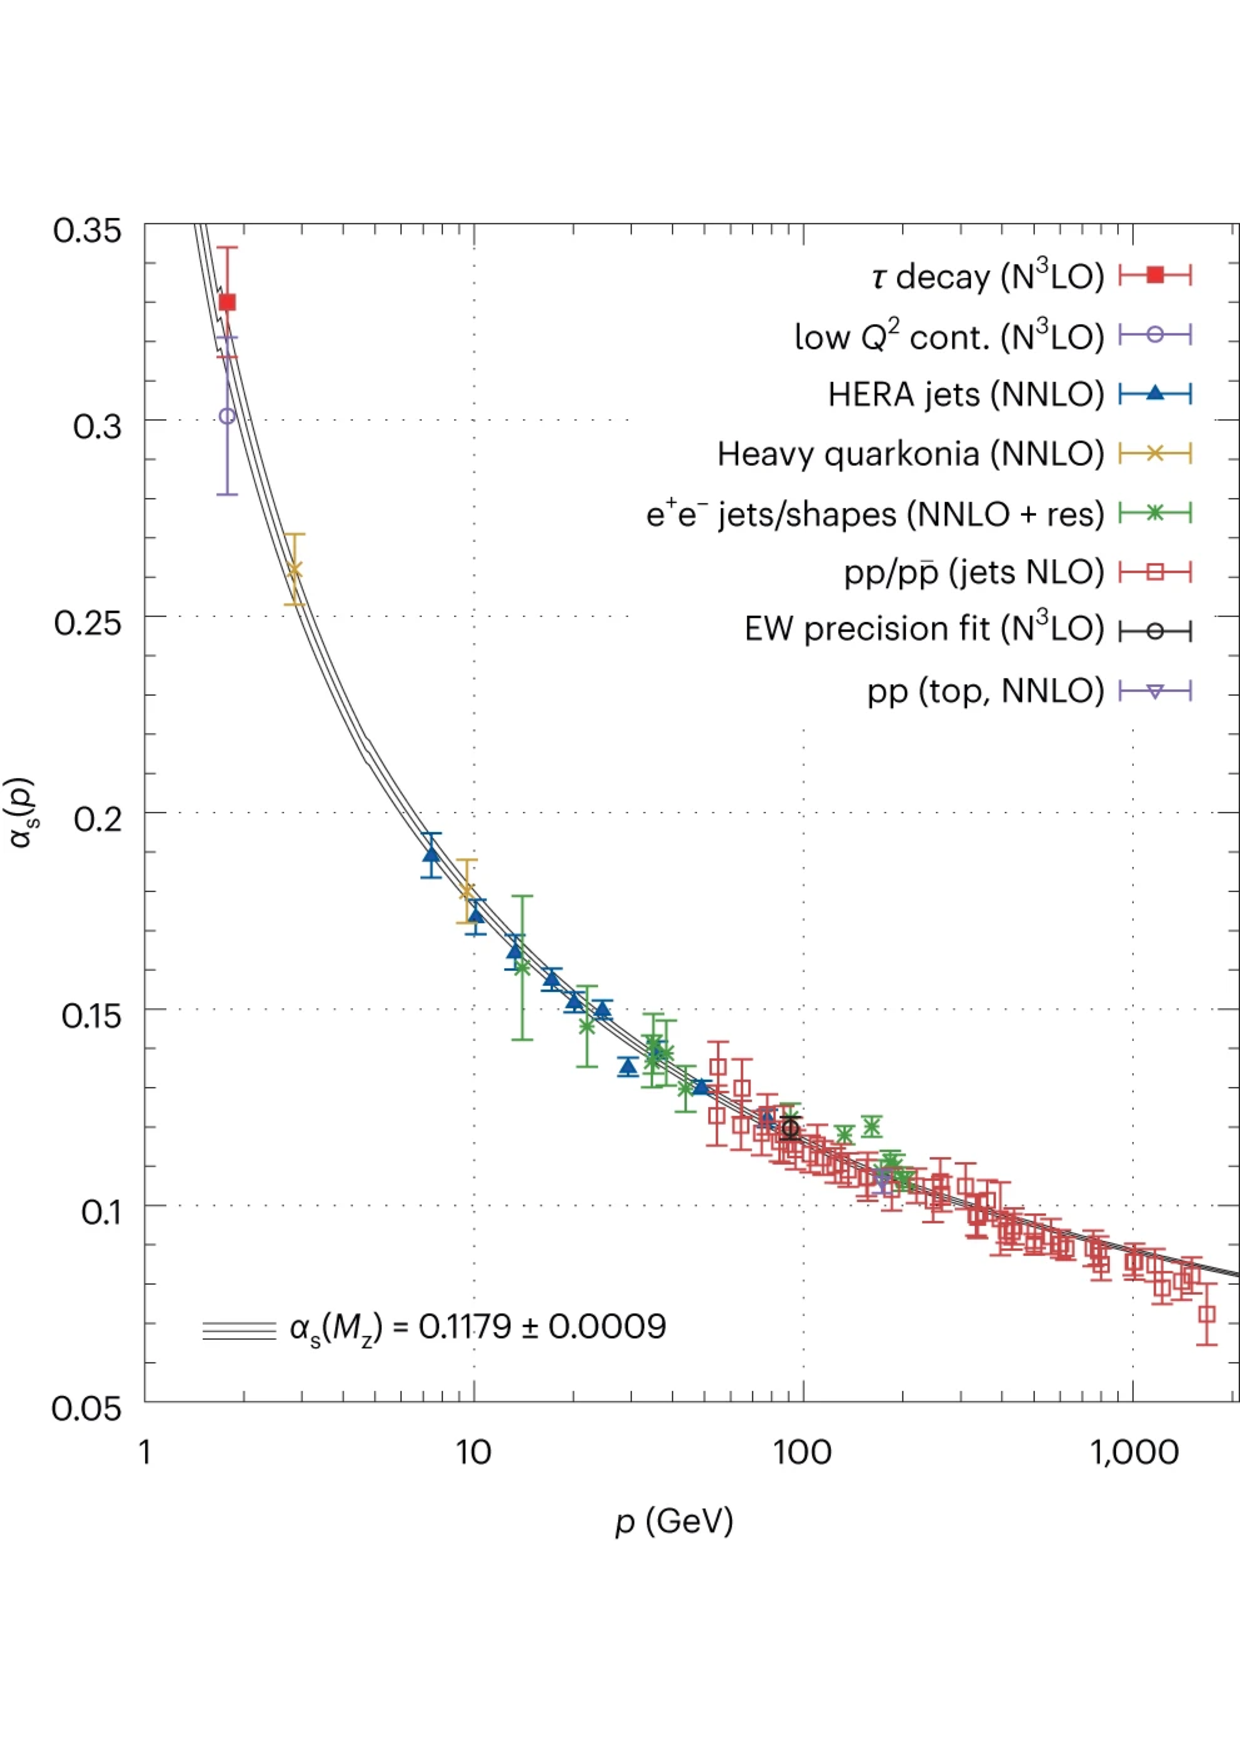
\includegraphics[width=0.5\textwidth]{figures/01-SM-03-SM/qcd/qcd_running}
	\caption{The theoretically predicted running of the strong coupling $\alpha_s = \cnicefrac{g_s^2}{4\pi}$ as a function of the energy scale along with experimental measurements, reproduced from Ref.~\cite{Boito:2023lzf}.}
	\label{fig:01_sm_qcd_running}
\end{figure}

The $\mathcal O(1)$ coupling strength means that the standard perturbative techniques we have discussed are not applicable at our usual energy scales; instead, we must rely on nonperturbative techniques such as numerical simulations of QCD on a discretized spacetime lattice (see e.g. Schwartz~\cite{Schwartz:2014sze} Chapter 25).
Because of this, QCD is one of the least understood and most exciting areas of study in modern physics.

% \TODO{Organization of this section}


\subsection{Asymptotic freedom and confinement}
\label{sec:01_sm_qcd_asymptotic}

As discussed above, a key phenomenological characteristic of the strong force is asymptotic freedom, wherein at high energies quarks and gluons behave as free particles.
This also means that perturbative techniques can be applied at high energies; indeed, we can derive an analogous $\cnicefrac{1}{r^2}$ ``Coulomb force'', based on tree-level quark-quark scattering amplitudes, for quarks at very short distances.
This force turns out to always be attractive between quarks and antiquarks, as well as between two or even three quarks in different color states: the ``aim'' of the force appears to always be to form color-neutral bound states.
These are called \textit{mesons} for the case of an antiquark and quark pair, and \textit{baryons} for three quarks.

At longer distances we enter the strong-coupling and nonperturbative regime, in which the dynamics are harder to understand.
However, through lattice QCD simulations, we are able to see the emergence of a ``flux tube'' pulling quarks together as they are pushed apart, as shown in Figure~\ref{fig:01_sm_qcd_fluxtubes}.
This phenomenon is referred to as \textit{confinement}, and it means we can never observe free quarks or gluons outside high-energy colliders.
Both the long- and short-distance behavior of the strong force conspire to always confine quarks in color-neutral hadrons.
The scale of confinement is naturally set by $\Lambda_{\mathrm{QCD}} \approx 200 \MeV$, which is hence roughly the radius of the proton and other hadrons ($1$fm in SI).

\begin{figure}[ht]
	\centering
	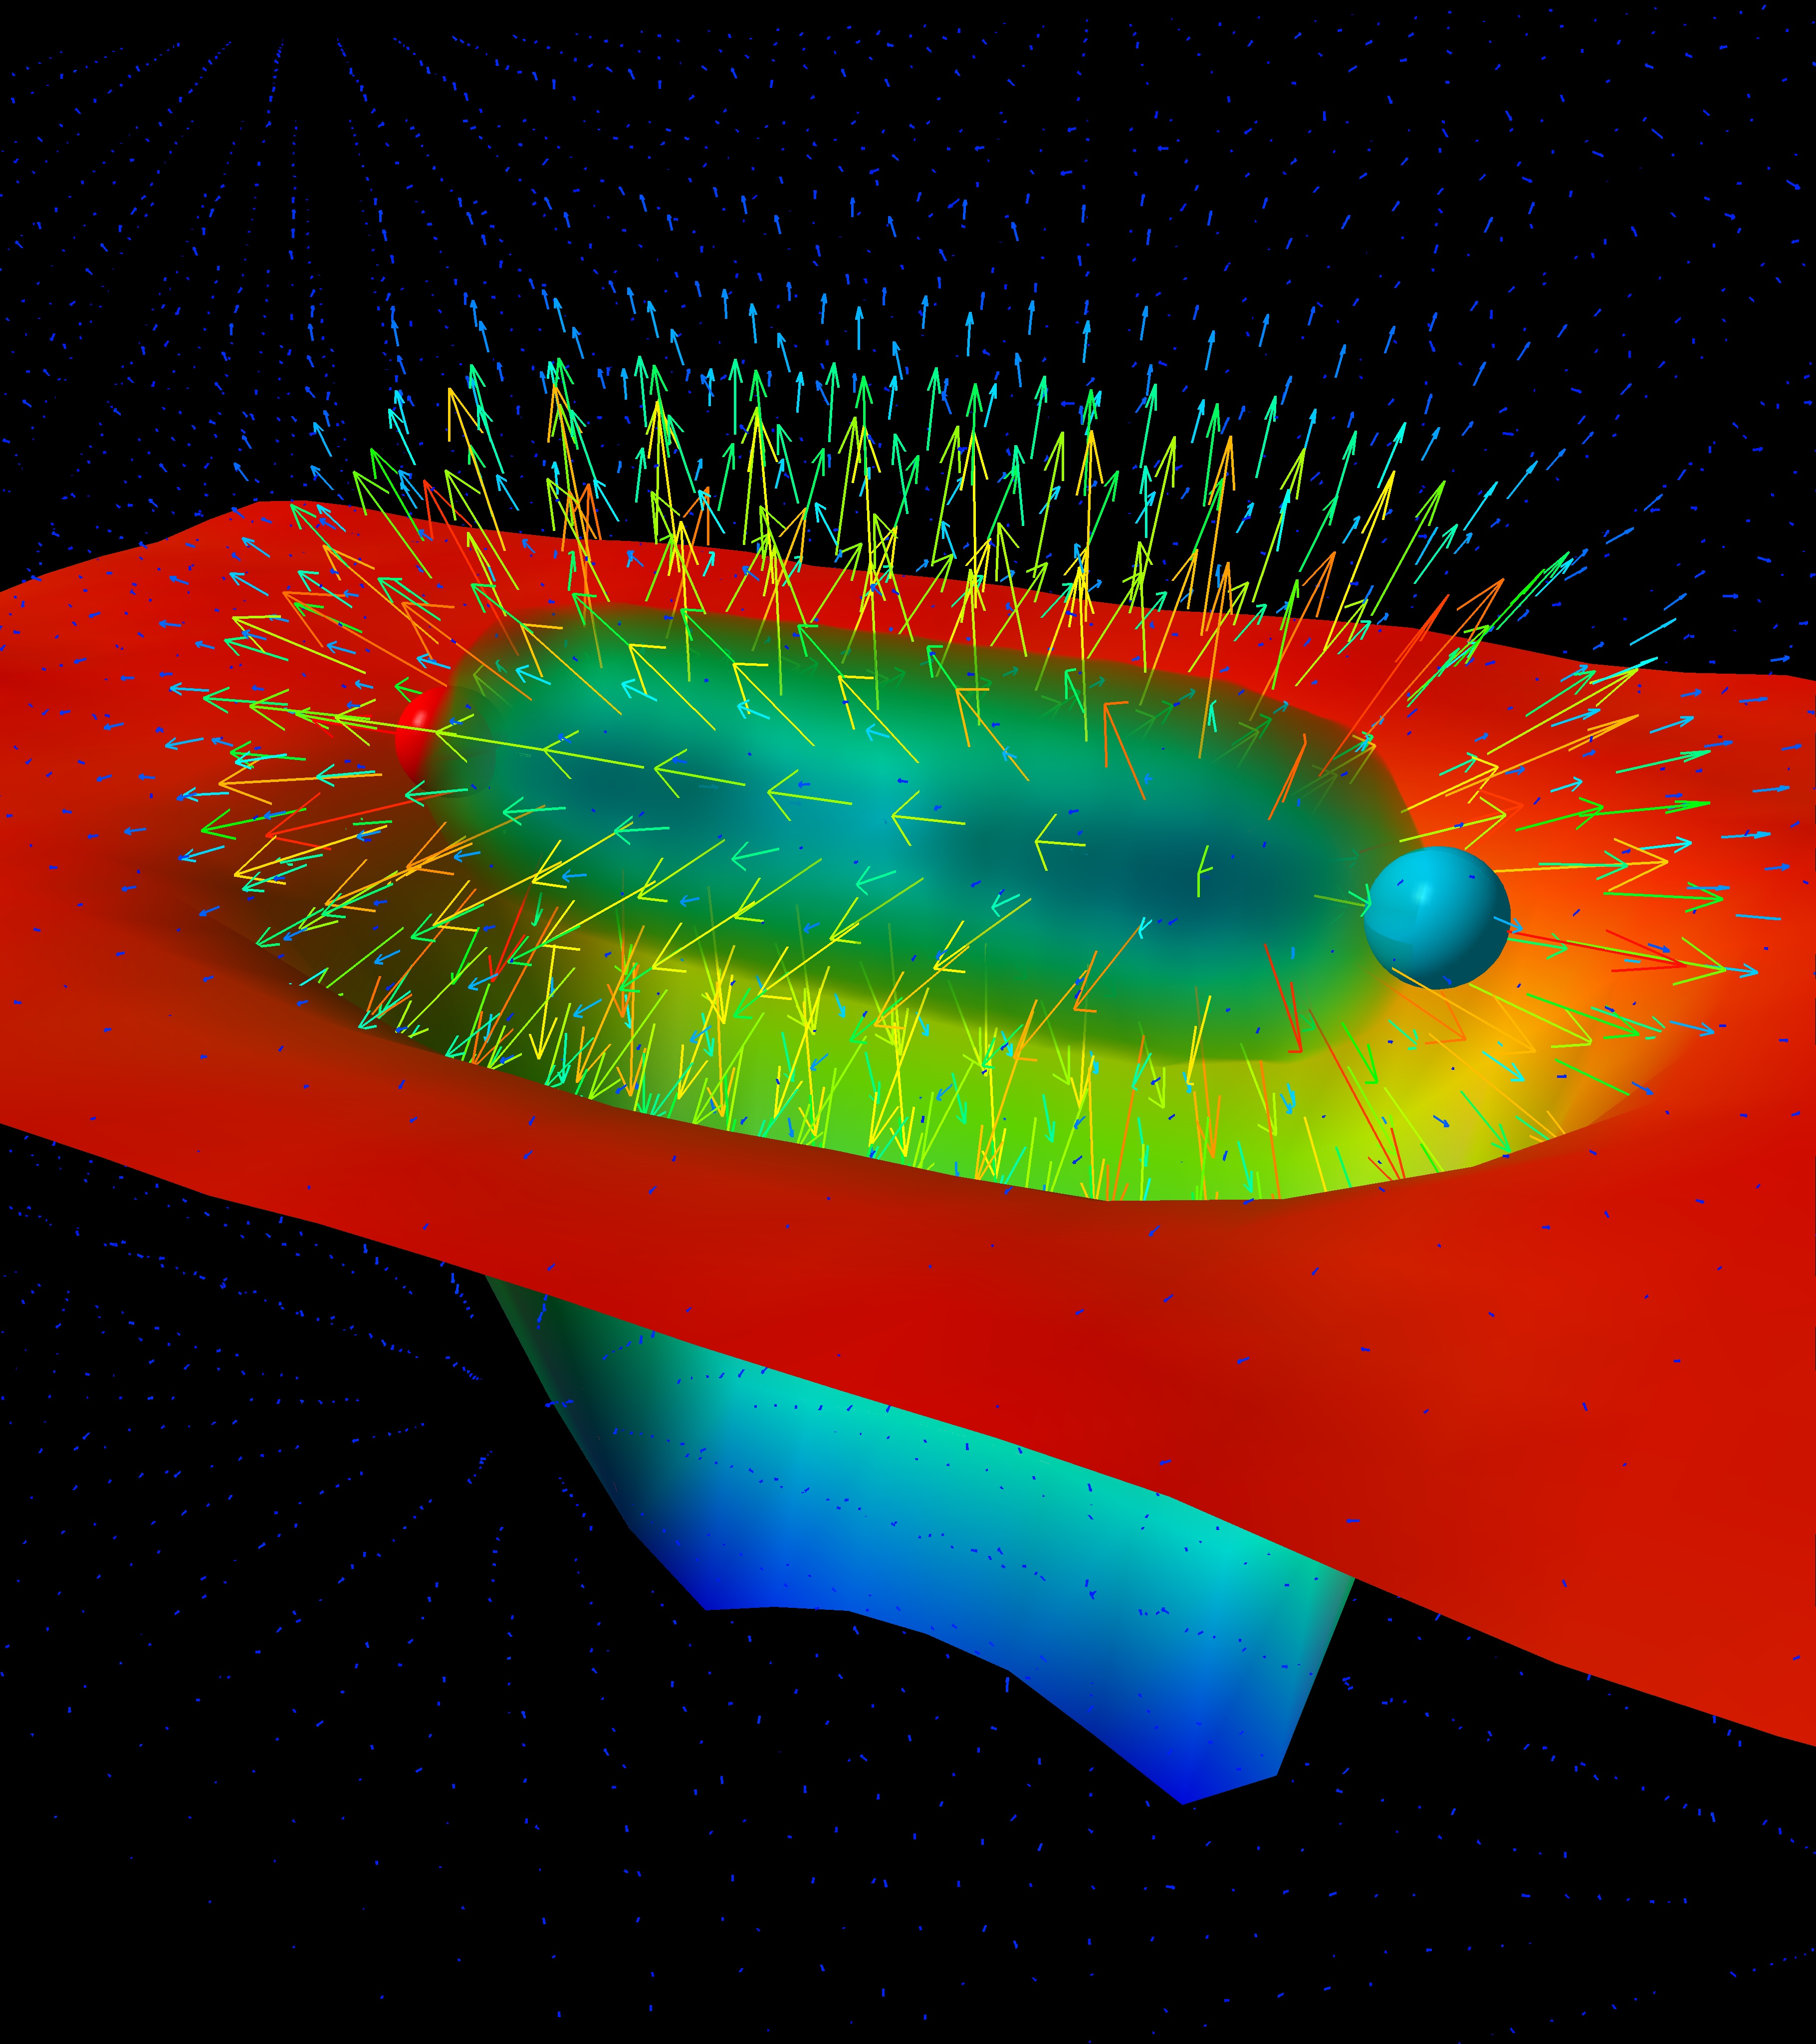
\includegraphics[height=7cm]{figures/01-SM-03-SM/qcd/FluxTube.jpg}
	\hspace{2mm}
	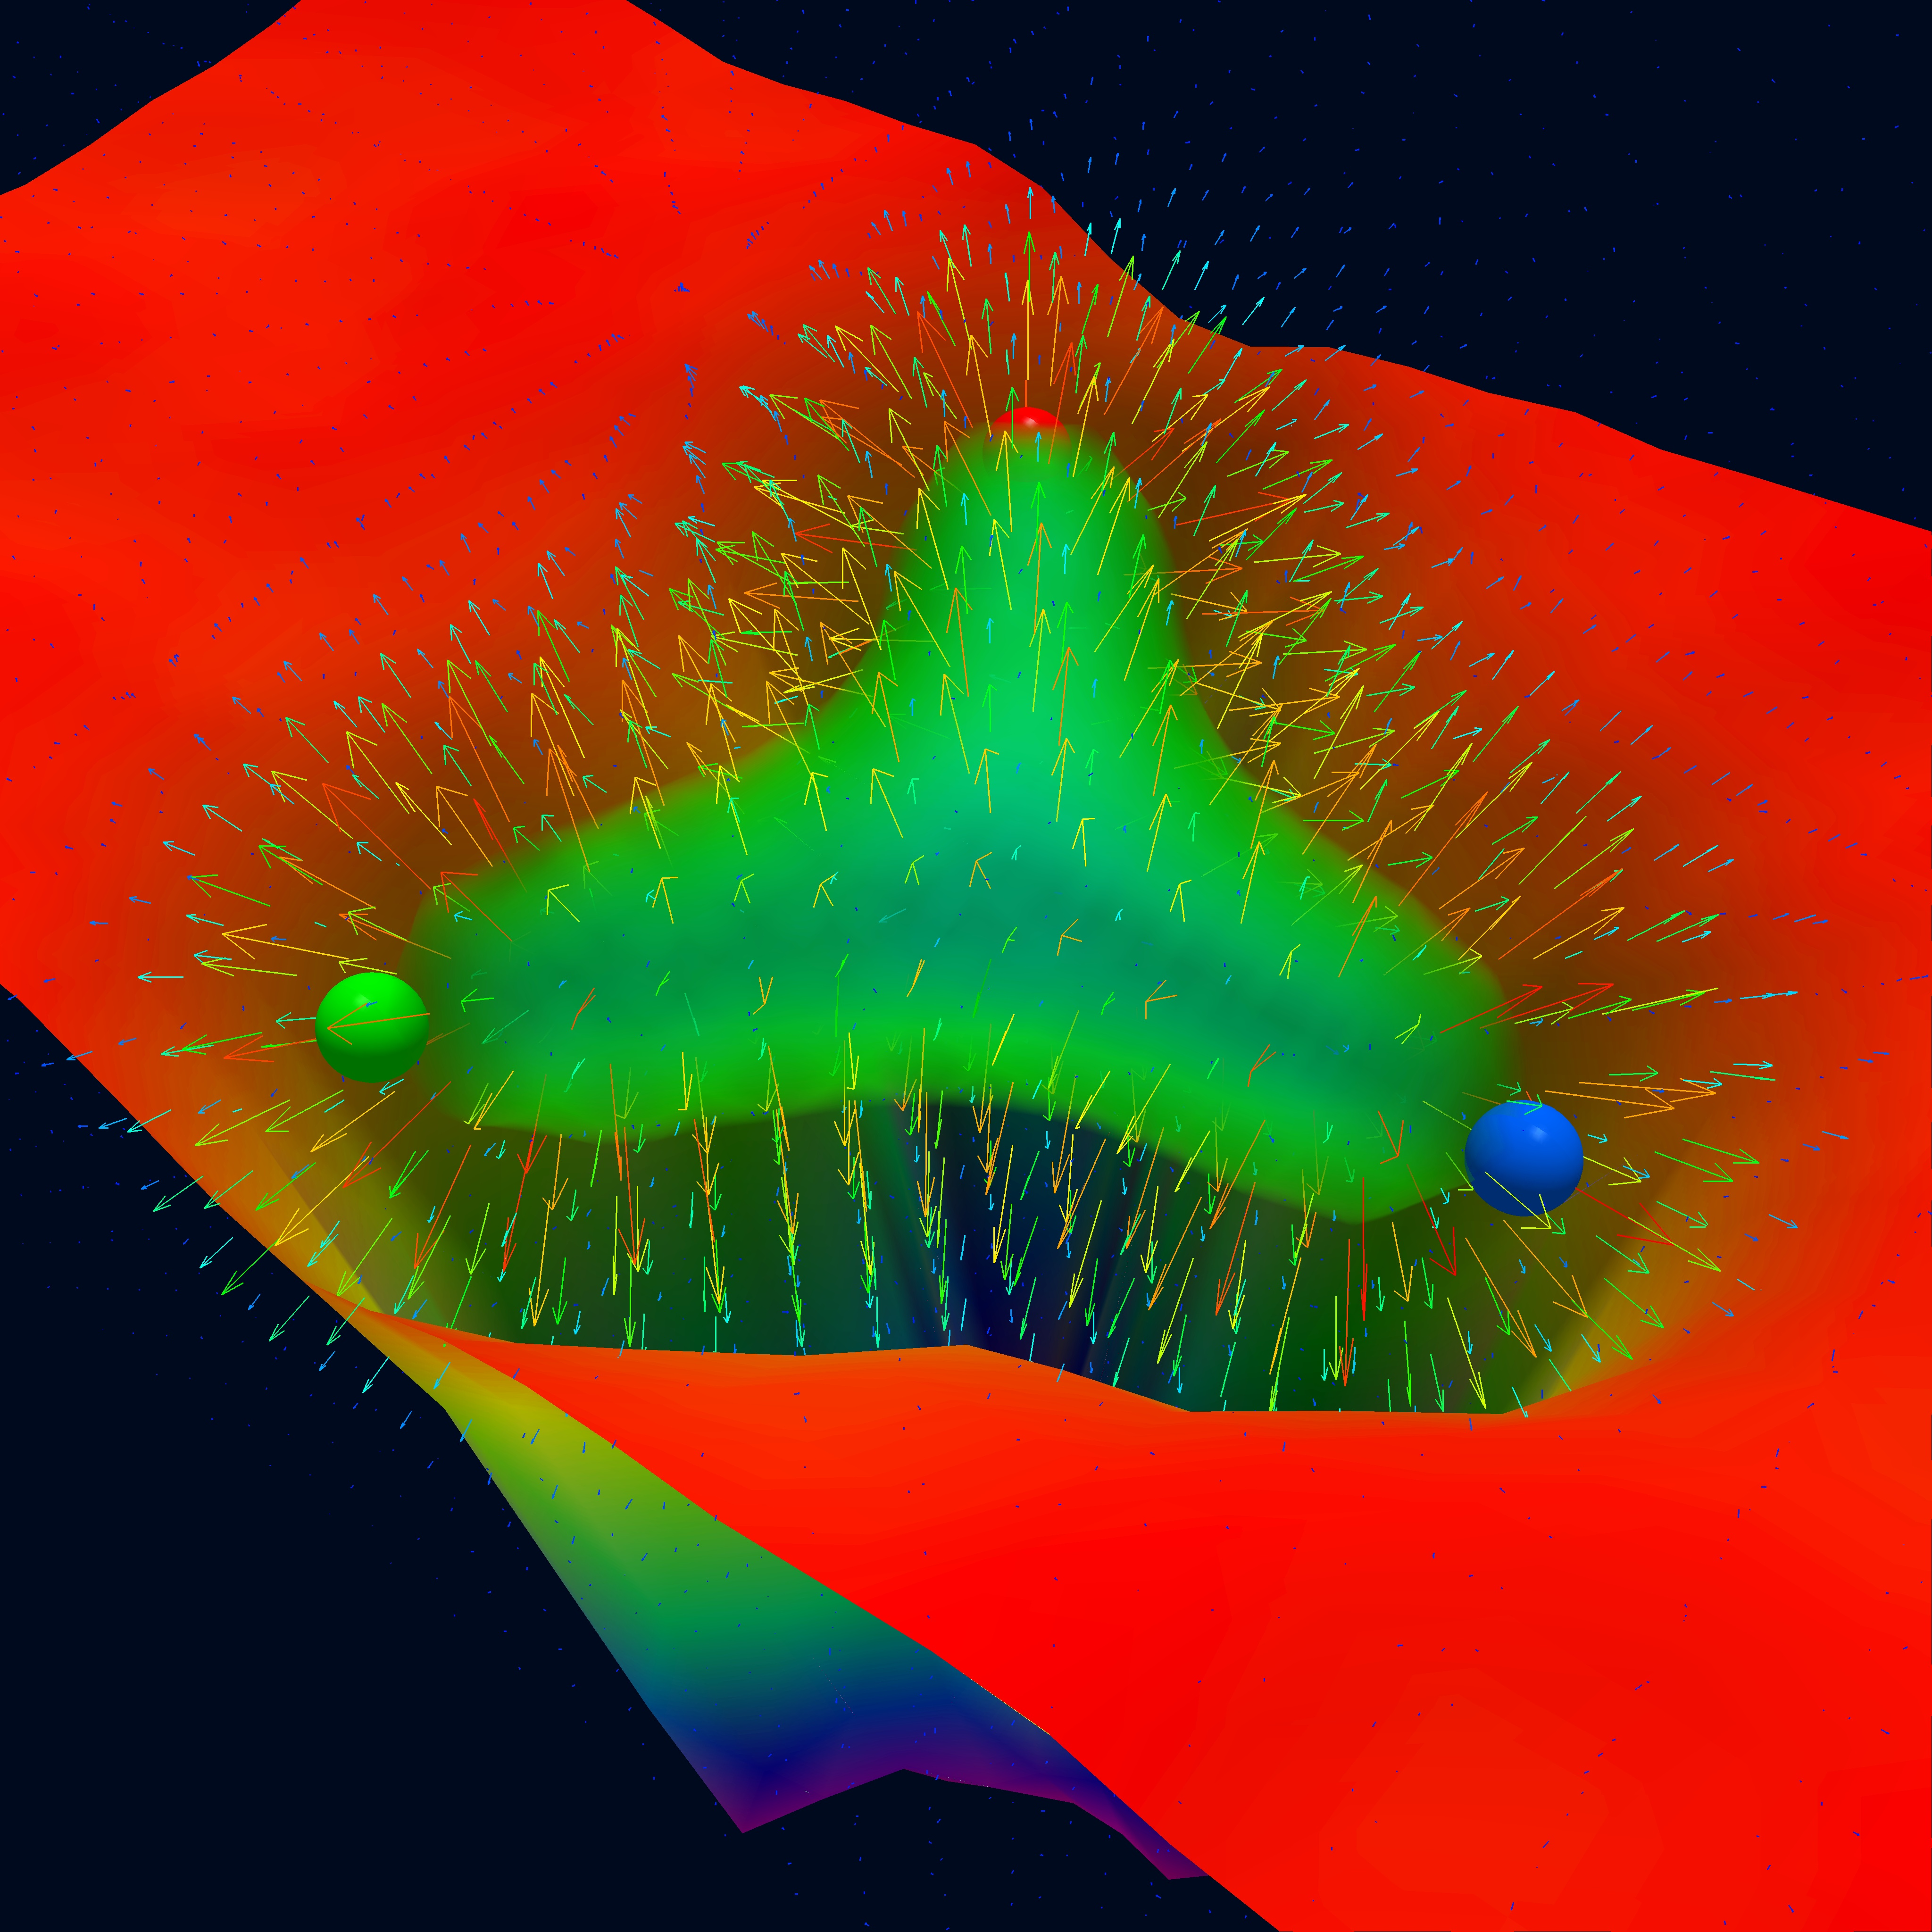
\includegraphics[height=7cm]{figures/01-SM-03-SM/qcd/VacuumRespAction16t32_YshapeCSSMcover.jpg}
	\caption{``Flux tubes'' between a quark and anti-pair inside a meson (left) and three quarks in a proton (right), reproduced from Refs.~\cite{Bissey:2006bz, LeinweberVisualQCD}.}
	\label{fig:01_sm_qcd_fluxtubes}
\end{figure}


\subsection{Quarks and the eightfold way}
\label{sec:01_sm_quarks}

Since their discovery in the 1920s and 30s, the proton and neutron and were believed to be elementary particles along with the electron and photon.
In fact, due to confinement, the first experimental evidence of quarks was not found until the 1960s.
However, already in 1932, the remarkably similar masses of the two nucleons surprised physicists and led Heisenberg, Wigner, and others to hypothesize an underlying \SU[2] symmetry between them (later named \textit{isospin})~\cite{Heisenberg1932, Wigner1937}.
The intrigue only increased in the next decades, during which new cosmic ray, cyclotron, and bubble chamber experiments discovered a veritable ``zoo'' of hadrons, exemplified by a 1964 table of particles in Figure~\ref{fig:01_sm_qcd_particle_zoo}.
While all appeared elementary, several had surprisingly similar properties such as mass and spin, and could also be grouped into invariant subspaces of the isospin group.

\begin{figure}[ht]
	\centering
	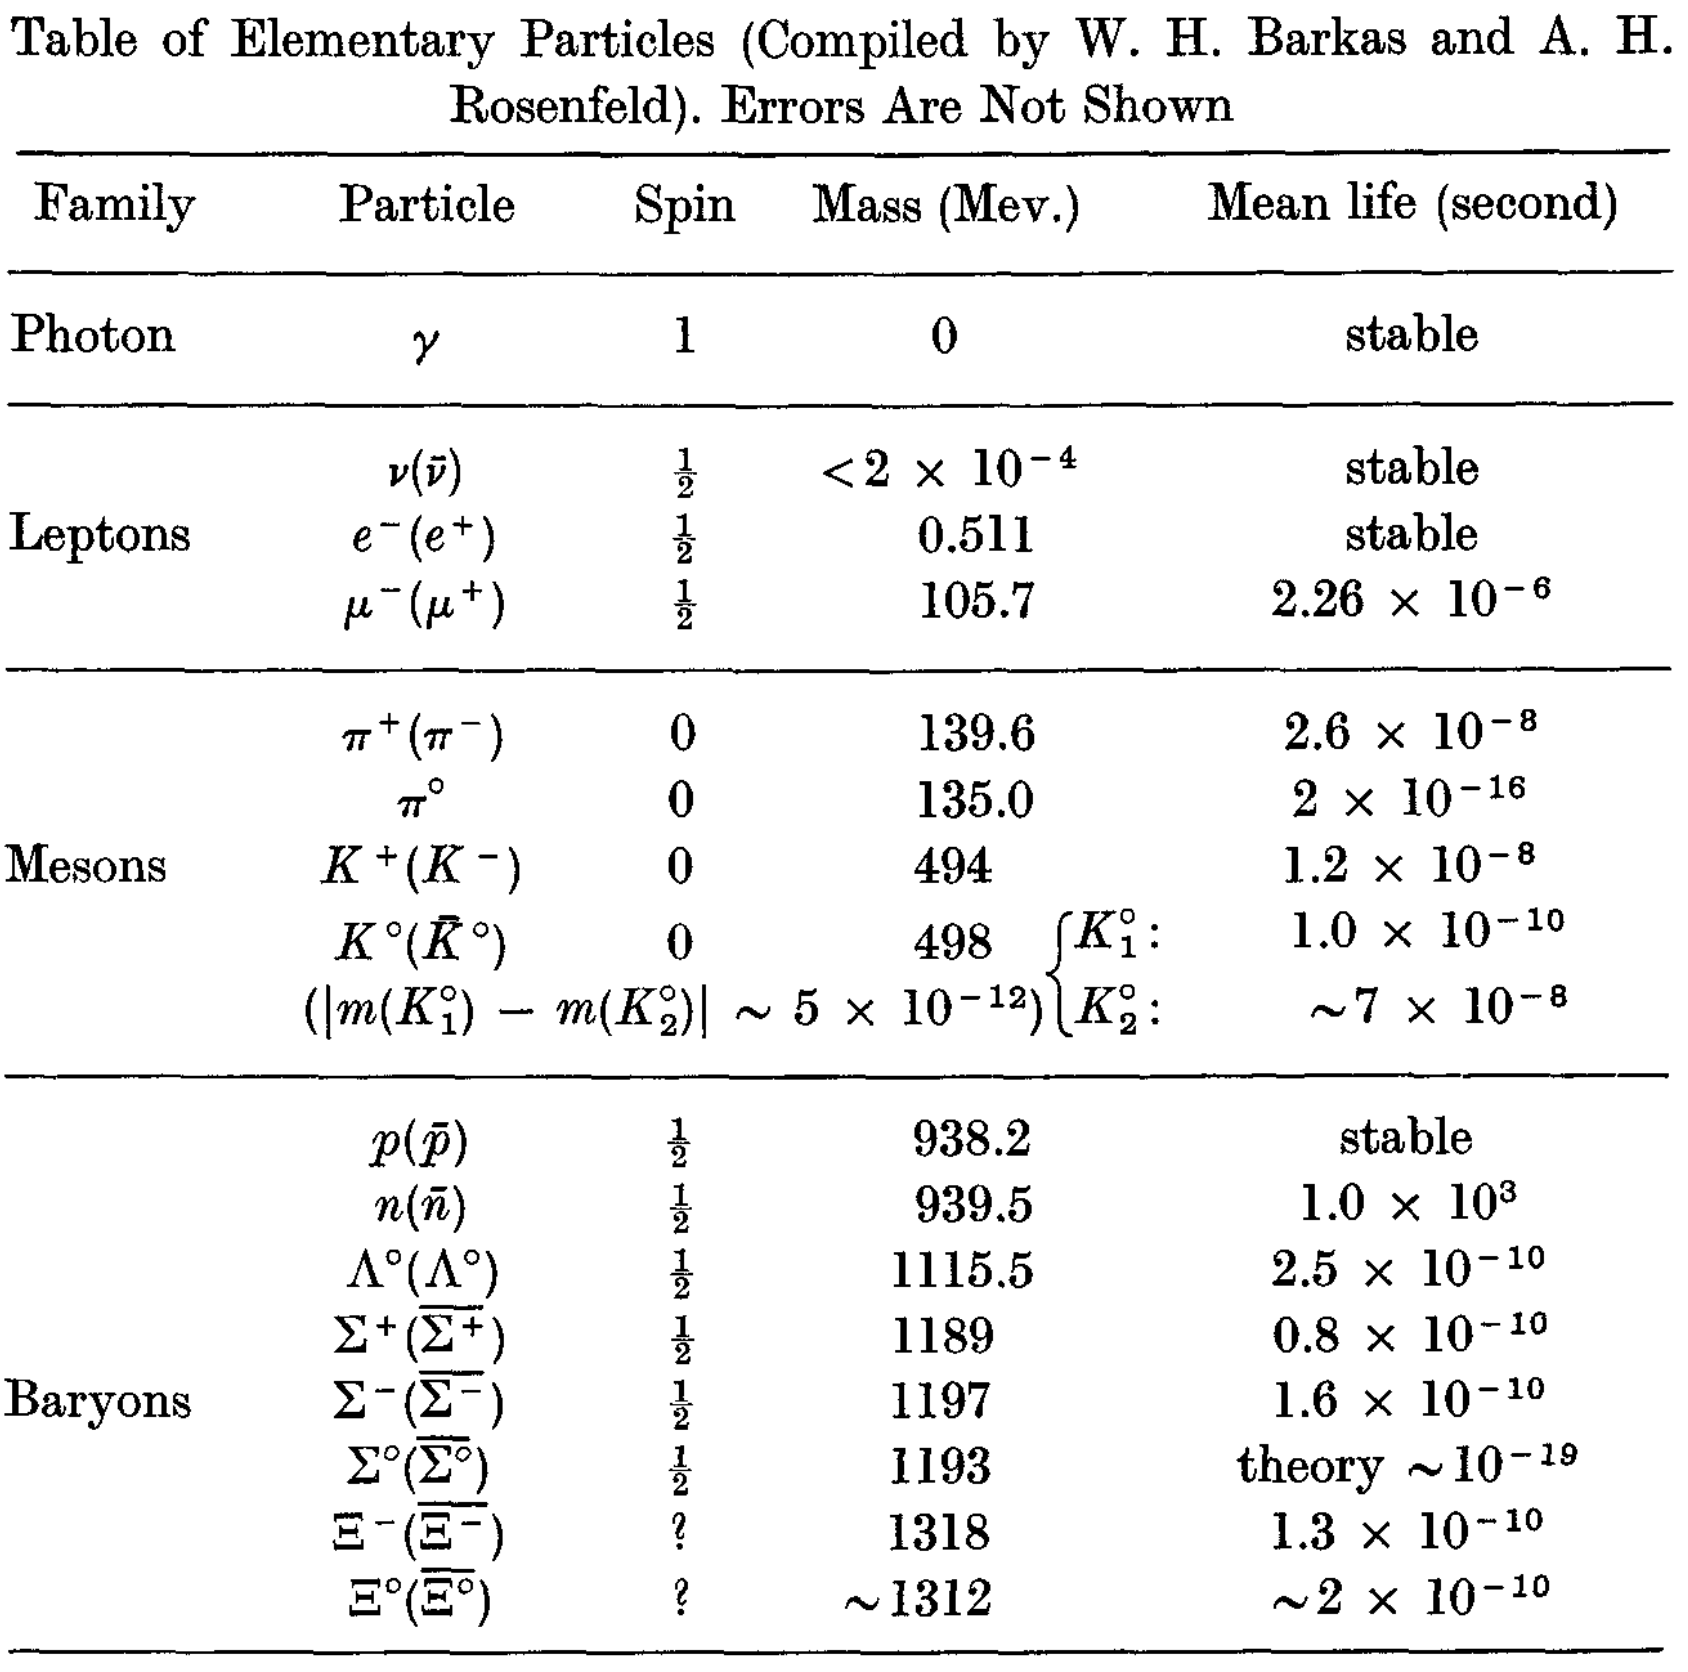
\includegraphics[width=0.8\textwidth]{figures/01-SM-03-SM/qcd/table_elementary_particles_sakurai.png}
	\caption{A table of what were considered to be elementary particles in 1964, reproduced from Ref.~\cite{Sakurai:2015gmk}.}
	\label{fig:01_sm_qcd_particle_zoo}
\end{figure}

In 1961, Murray Gell-Mann and Yuval Ne'eman independently realized that the new hadrons could elegantly fit into representations of a larger symmetry group, \SU[3]~\cite{Gell-Mann:1961omu, Neeman:1961jhl}.
Gell-Mann and George Zweig in 1964 then independently showed that this could be explained physically by hadrons being composed of combinations of three fundamental particles, named the ``up'', ``down'', and ``strange quarks'', with the former two carrying isospin up and down, respectively~\cite{Gell-Mann:1964ewy, Zweig:1964jf}.
% \footnote{Although, interestingly, Gell-Mann himself thought of them as mathematical conveniences than real particles.}
Gell-Mann named this model the ``eightfold way'' (since $\dim (\SU[3]) = 8$) and was awarded the Nobel Prize in 1969 for this work.

Examples of baryons (three-quark hadrons) in the octet and decuplet (dimension 8 and 10, respectively) representations of $\SU[3]$ are shown in Figure~\ref{fig:01_sm_qcd_eightfoldway}, sorted by their isospin along the ``z'' axis ($I_3 = $ \# of up quarks - \# of down quarks) and strangeness ($S = $ \# of strange quarks).
Note that this \SU[3] symmetry is only approximate; it is broken by the different masses of the quarks.
However, their significantly smaller masses compared to $\Lambda_{\mathrm{QCD}}$ mean it remains a useful symmetry for categorizing hadrons.
On the other hand, broader ``symmetries'' such as \SU[4] through \SU[6] including the heavier charm, bottom and top quarks are broken so heavily by their higher masses that they are not helpful for characterizing the heavier hadrons.

\begin{figure}[ht]
	\centering
	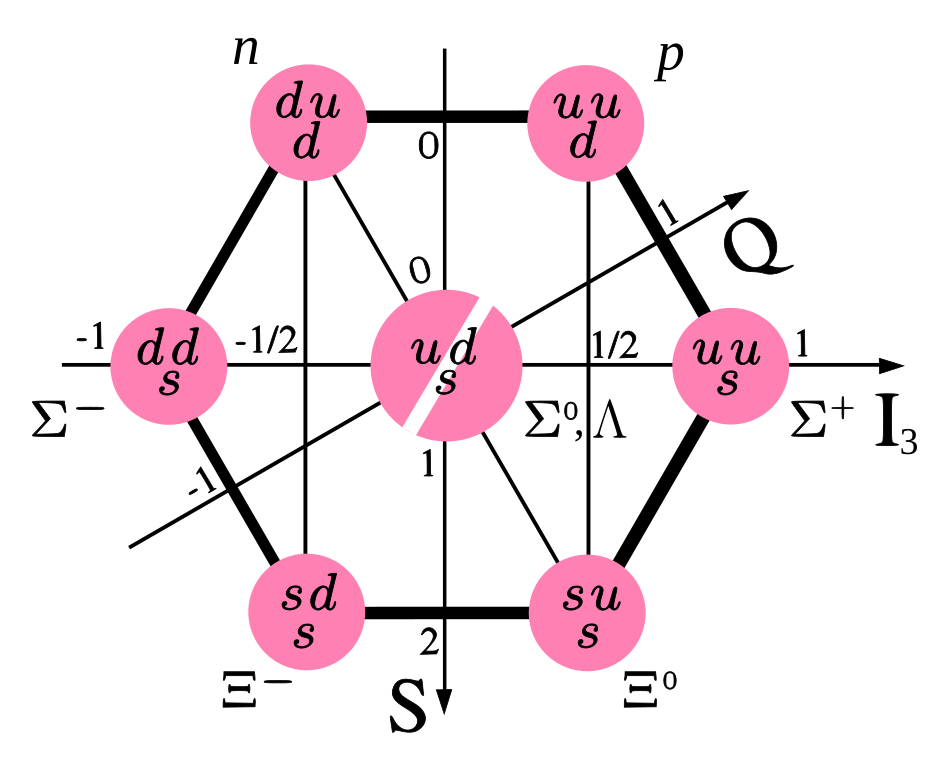
\includegraphics[width=0.45\textwidth]{figures/01-SM-03-SM/qcd/Baryon-octet-small.svg.png}
	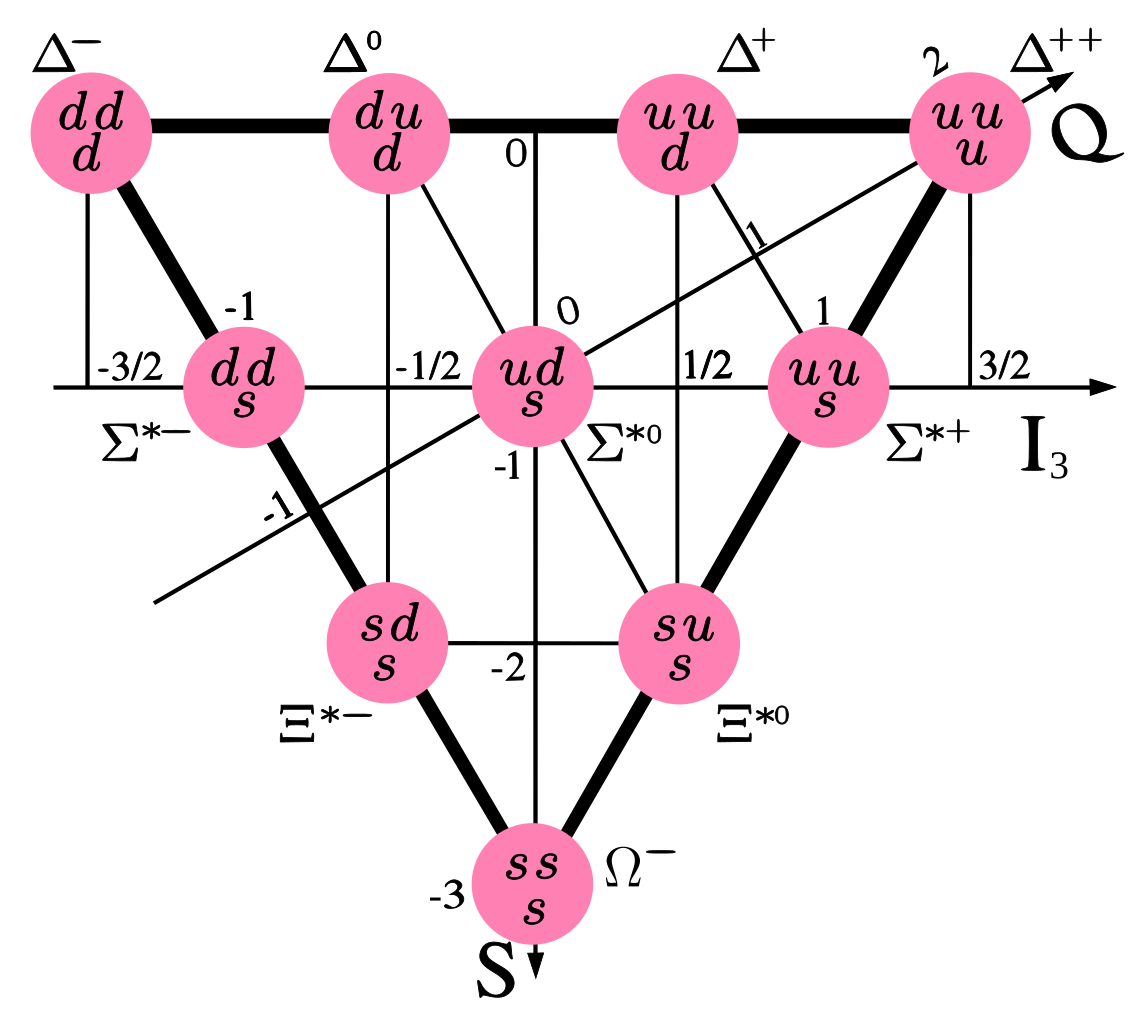
\includegraphics[width=0.45\textwidth]{figures/01-SM-03-SM/qcd/Baryon-decuplet-small.svg.png}
	\caption{Baryons in the octet (left) and decuplet (right) representations of $\SU[3]$, reproduced from Ref.~\cite{enwiki:1243626239}.}
	\label{fig:01_sm_qcd_eightfoldway}
\end{figure}

This fourth ``charm'' quark was notably predicted by Sheldon Glashow, John Iliopoulos, and Luciano Maiani in 1970 to explain the observed suppression of $Z$-boson-mediated flavor-changing neutral currents~\cite{Glashow:1970gm} (and also to match the number of known leptons at the time).
This, and the quark model as a whole, was famously validated by the discovery of a $3.1 \GeV$ charm-anti-charm bound state, named the $J/\psi$ meson, simultaneously by Burton Richter's team at the Stanford Linear Accelerator Center (SLAC) and Samuel Ting's team at Brookhaven National Laboratory in 1974~\cite{SLAC-SP-017:1974ind, E598:1974sol}, both of whom received the Nobel Prize in 1976.

A year before this, Makoto Kobayashi and Toshihide Maskawa had proposed the existence of a \textit{third} generation of quarks to explain the observed CP-violation in weak interactions~\cite{Kobayashi:1973fv}.
This proposal gained more traction after the $J/\psi$ discovery, as well as the discovery of a third-generation lepton, the $\tau$, by Martin Lewis Perl's team in electron-positron collisions at SLAC between 1973 and 1977~\cite{Perl:1975bf}.

In the end, both third generation quarks were discovered at the Fermi National Accelerator Laboratory (Fermilab): first the bottom quark in 1977 by Leon Lederman's team on the E288 experiment~\cite{E288:1977xhf}; and then, much later, the top quark in 1995 by the CDF and DØ experiments at the Tevatron~\cite{CDF:1995wbb, D0:1995jca}.
The bottom quark was discovered indirectly, as with the charm quark, through the observation of a bottom quark-antiquark bound state called bottomium, or the $\Upsilon$ meson, in proton-nucleon collisions.

The top quark, on the other hand, is highly unique because of its high $173 \GeV$ mass, and it decays too quickly to form bound states.
Hence, it is the only quark to have been observed ``directly'', through its decays to a $W$ boson and a bottom quark.
It is the heaviest known elementary particle, which is why its discovery required the 1\TeV center-of-mass energy proton-antiproton collisions of the Tevatron.
The unique nature of the heavy quarks leads to a rich phenomenology at high energy colliders such as the LHC, particularly in the context of the \textit{jets} they form (Section~\ref{sec:01_sm_qcd_jets}).

% and hence could be discovered directly through its decays to a $W$ boson and a bottom quark in proton-antiproton collisions.
% Indeed, because of its high mass, it is unable to form bound states, decaying too quickly, and is the only quark that can decay directly to other particles.
% in proton-nucleon collisions which produced a bottom-antibottom bound state called bottomium, or the $\Upsilon$ meson~\cite{E288:1977xhf}

% in proton-antiproton collisions

% The top quark turns out to be highly unique due to its high $173 \GeV$ mass.
% It is the heaviest known elementary particle, which is why its discovery required the 1\TeV center-of-mass energy collisions of the Tevatron.
% It cannot form hadronic bound states due to its short lifetime, and is the only quark that can directly decay to other particles (primarily to a $W$ boson and a bottom quark).
% The unique nature of the heavy quarks leads to a rich phenomenology at high energy colliders such as the LHC, particularly in the context of the \textit{jets} they form, as will be discussed in \TODO{??}.

\subsection{The parton model}
\label{sec:01_sm_qcd_quarks_parton}

Some physicists, including Gell-Mann himself, initially believed quarks not to be real particles but simply mathematical conveniences to describe hadrons.
It was only through \textit{deep inelastic scattering} (DIS) experiments in the 1960s and 70s at SLAC --- in which high energy electrons were shot at protons (in the form of hydrogen) to probe their inner structure --- that it was confirmed that protons are indeed not point-like particles.

To explain this behavior, Richard Feynman and others proposed the \textit{parton model} of the proton (and other hadrons).
In this, protons are composed of point-like particles called \textit{partons} that are what actually interact with the electrons in DIS, as illustrated in Figure~\ref{fig:01_sm_qcd_dis}.
Though initially partons were abstract entities, we now identify them as the quarks and gluons of QCD.
At the energies required for DIS (and modern hadron colliders), the ``partonic'' cross-section of electron-parton scattering (or parton-parton scattering) ($\hat\sigma$) can be calculated using standard perturbation theory and Feynman diagrams.

To then derive the total ``hadronic'' electron-proton cross-section, we must integrate over all possible electron-parton interactions, weighted by the probability of finding a parton carrying a fraction $x$ of the proton's momentum at an energy scale $Q^2$.
This is described by the \textit{parton distribution functions} (PDFs) $f_i(x, Q^2)$, where $i$ represents the type of parton.
PDFs cannot be calculated perturbatively and must be determined from experimental data.
Examples for the proton at $Q^2 = 10 \GeV$ are shown in Figure~\ref{fig:01_sm_qcd_pdfs}; observe that the up and down quarks --- called the \textit{valence} or ``real'' quarks --- dominate at high $x$, while at lower $x$ there are gluons as well as other \textit{sea} (i.e., virtual) quarks.

The overall hadronic cross-section for DIS is thus:
\begin{equation}
	\label{eq:01_sm_qcd_sigma_ep}
	\sigma_{eh} = \sum_{i} \int_0^1 \dd x f_i(x, Q^2) \hat\sigma_{ei}(Q^2, \mu_r),
\end{equation}
where $\mu_r$ is the scale used for renormalization when calculating the partonic cross-sections.
The separation of the perturbative and nonperturbative parts of the cross-section is called \textit{factorization}, and the fact that this is possible is proved in the \textit{factorization theorem}~\cite{Collins:1989gx}.

As also illustrated in Figure~\ref{fig:01_sm_qcd_dis}, high energy hadron-hadron collisions such as those at the LHC involve a similar, but more complicated, interaction.
The corresponding cross-section involves integrating over two partons' momenta (one each from the two colliding hadrons):
\begin{equation}
	\label{eq:01_sm_qcd_sigma_pp}
	\sigma_{hh} = \sum_{i, j} \int_0^1 \dd x_1 \dd x_2 f_i(x_1, Q^2) f_j(x_2, Q^2) \hat\sigma_{ij}(Q^2, \mu_r).
\end{equation}
% where $\mu_r$ is the scale used for renormalization when calculating the partonic cross-sections.
This is known as the ``master formula'' for cross-sections at the LHC.\footnote{See lectures by Torsten Pfoh~\cite{Pfoh:2012Lectures} and Joey Huston~\cite{Huston:2018Lectures} for useful pedagogical discussions.}
PDFs are generally measured via DIS at electron-proton colliders, and are then crucial inputs to the above equation for hadron colliders.
There is also hope of deriving these through lattice QCD simulations.

\begin{figure}
	\centering
	\adjustbox{valign=m}{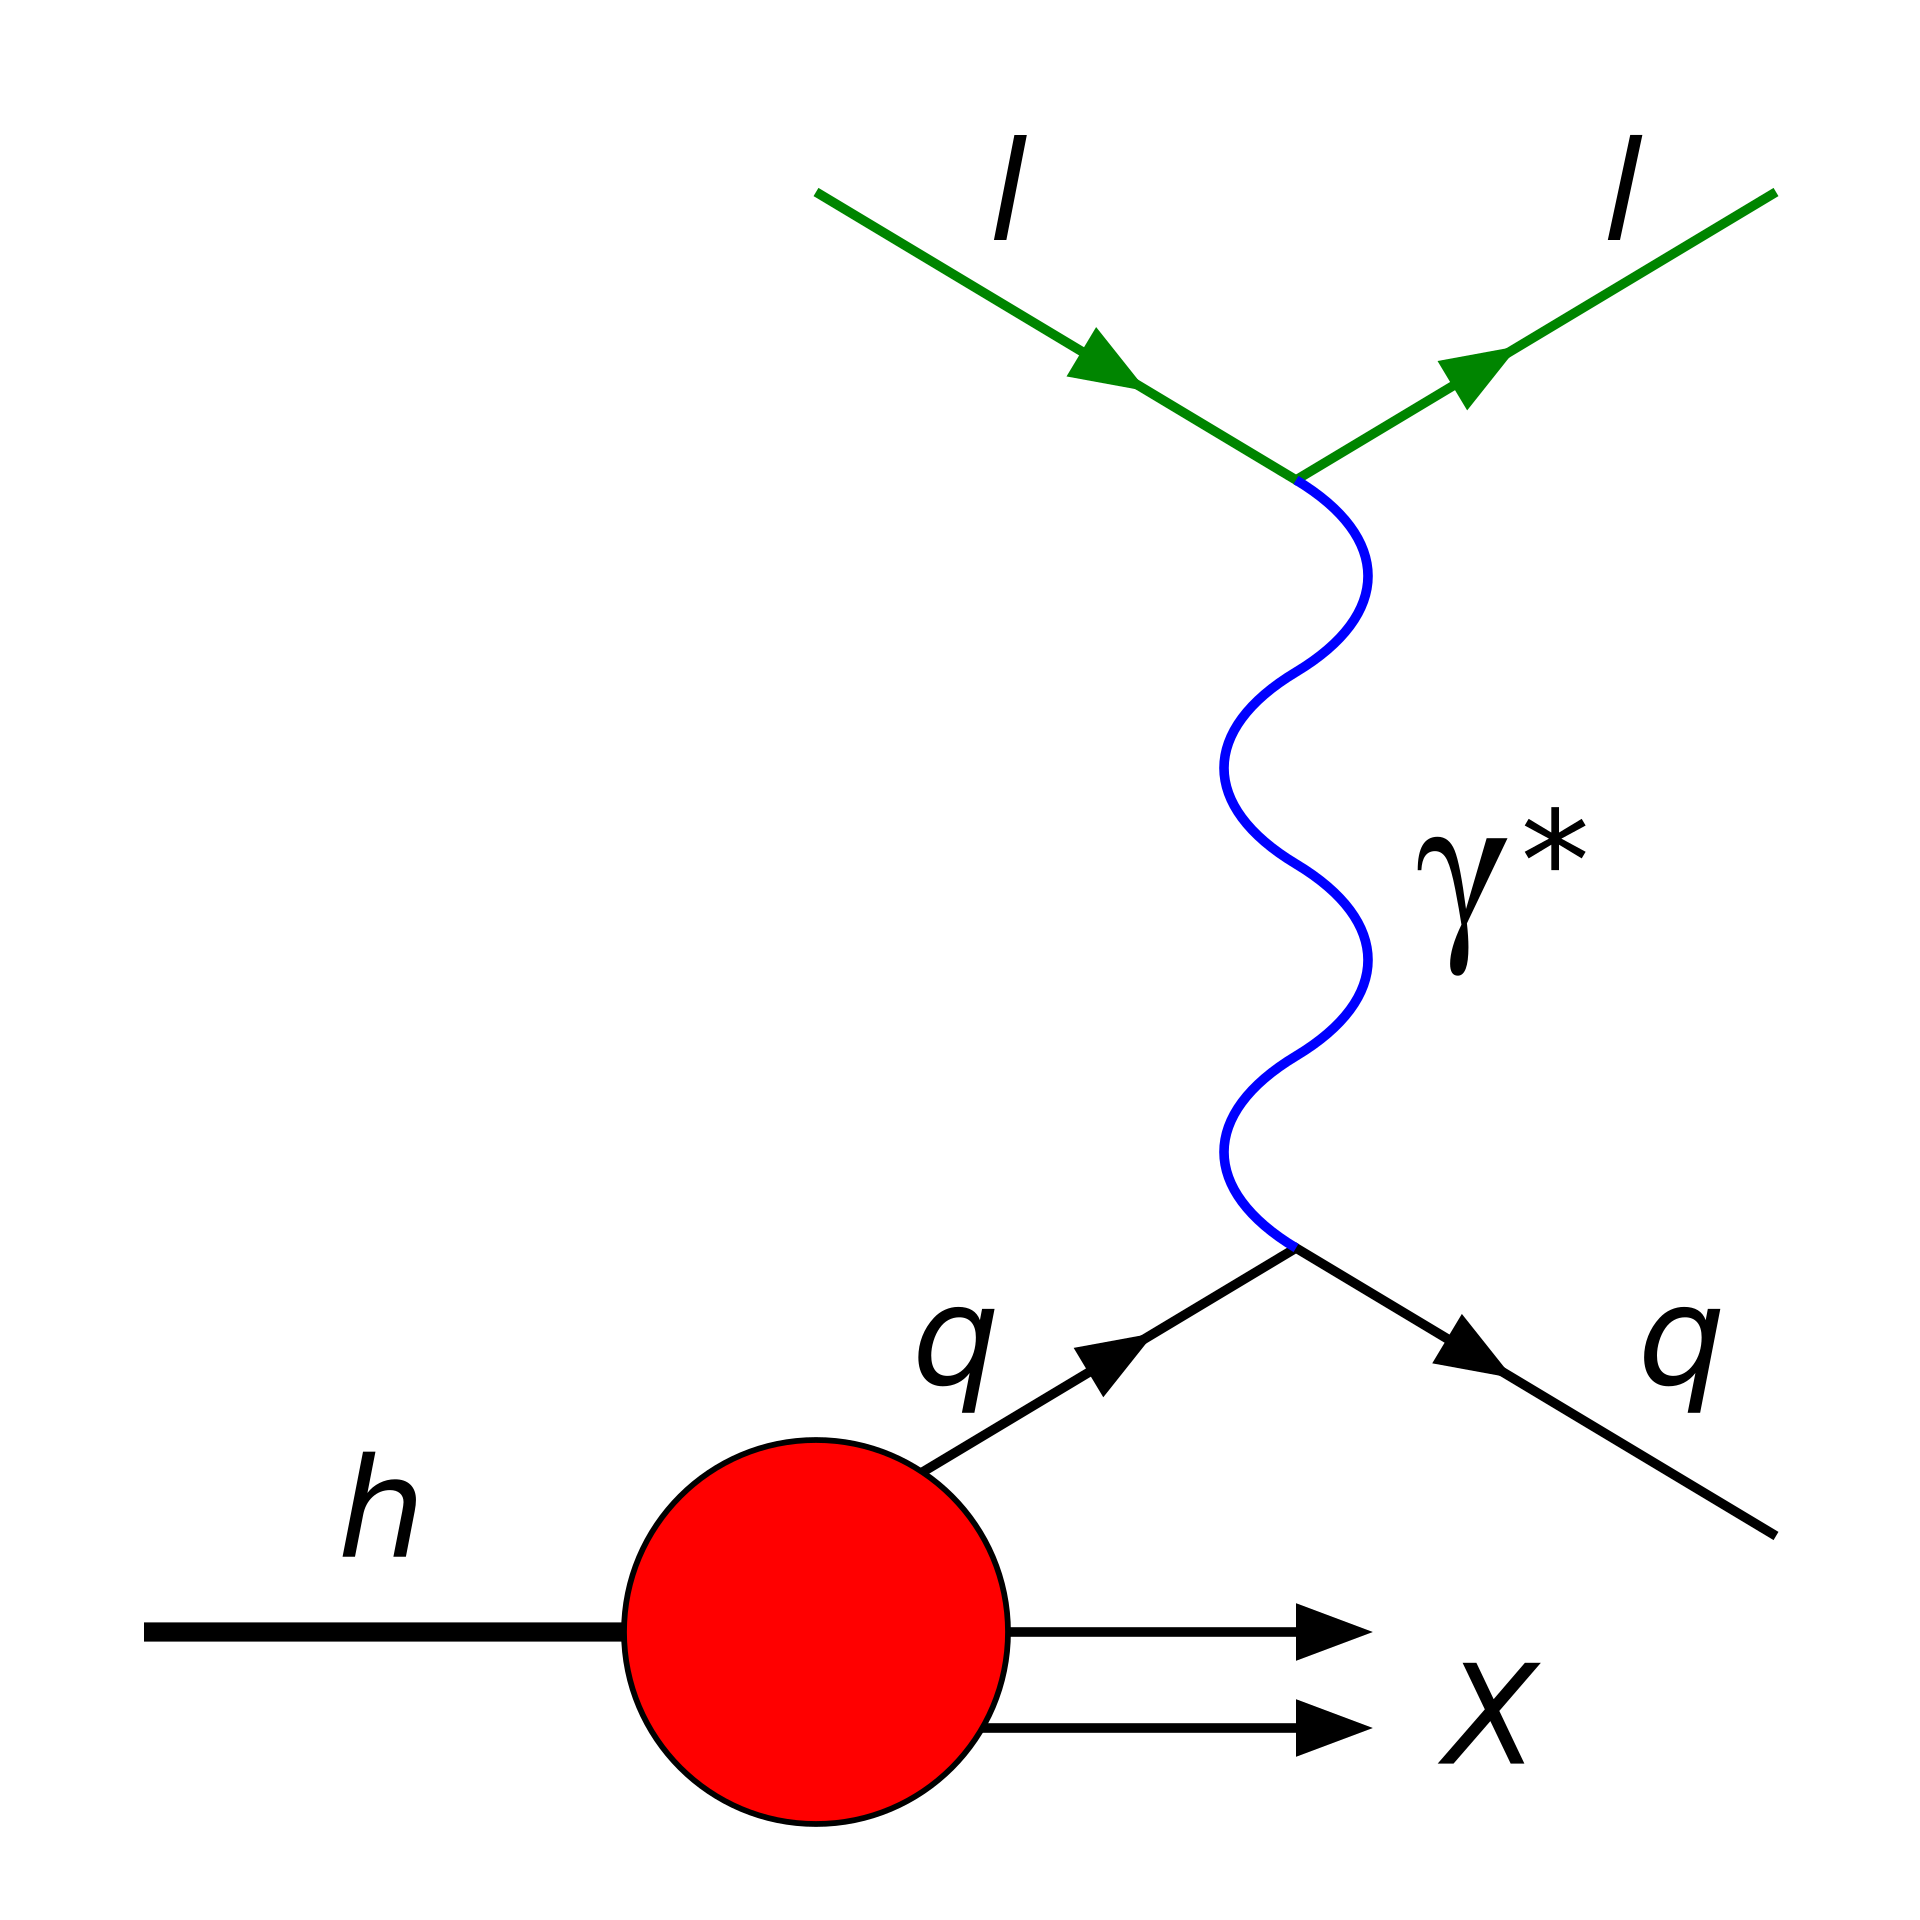
\includegraphics[width=0.3\textwidth]{figures/01-SM-03-SM/qcd/DIS.svg.png}}
	\hspace{1cm}
	\adjustbox{valign=m}{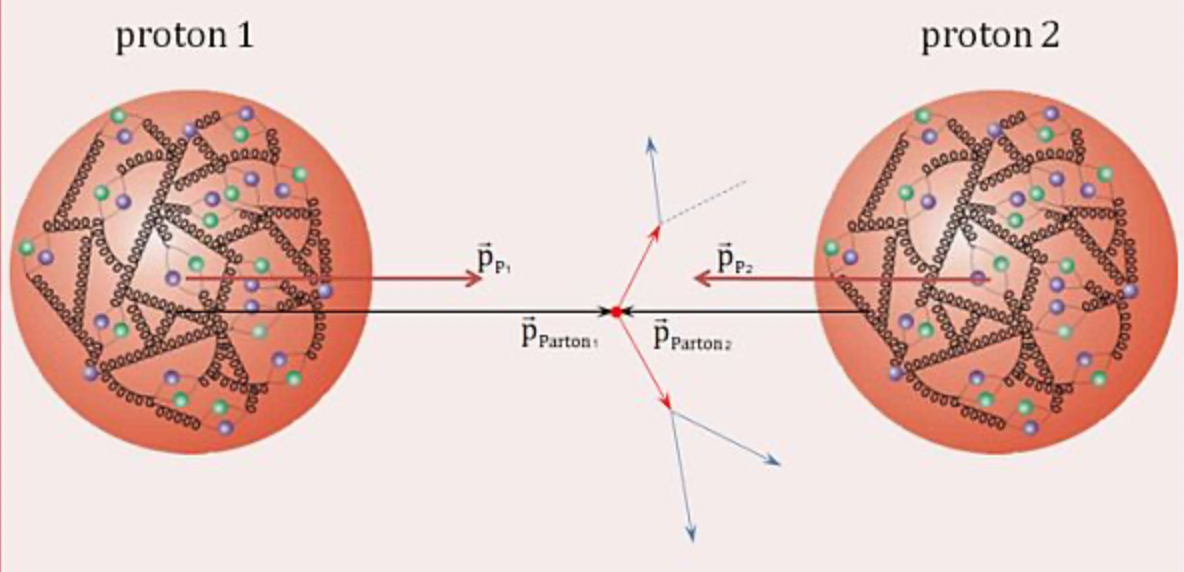
\includegraphics[width=0.45\textwidth]{figures/01-SM-03-SM/qcd/proton-proton.png}}
	\caption{Feynman diagram for deep inelastic scattering, reproduced from Ref.~\cite{enwiki:1240848406} (left) and an illustrative example of proton-proton collisions reproduced from Ref.~\cite{ATLAS:2024protoncollisions} (right).}
	\label{fig:01_sm_qcd_dis}
\end{figure}

\begin{figure}
	\centering
	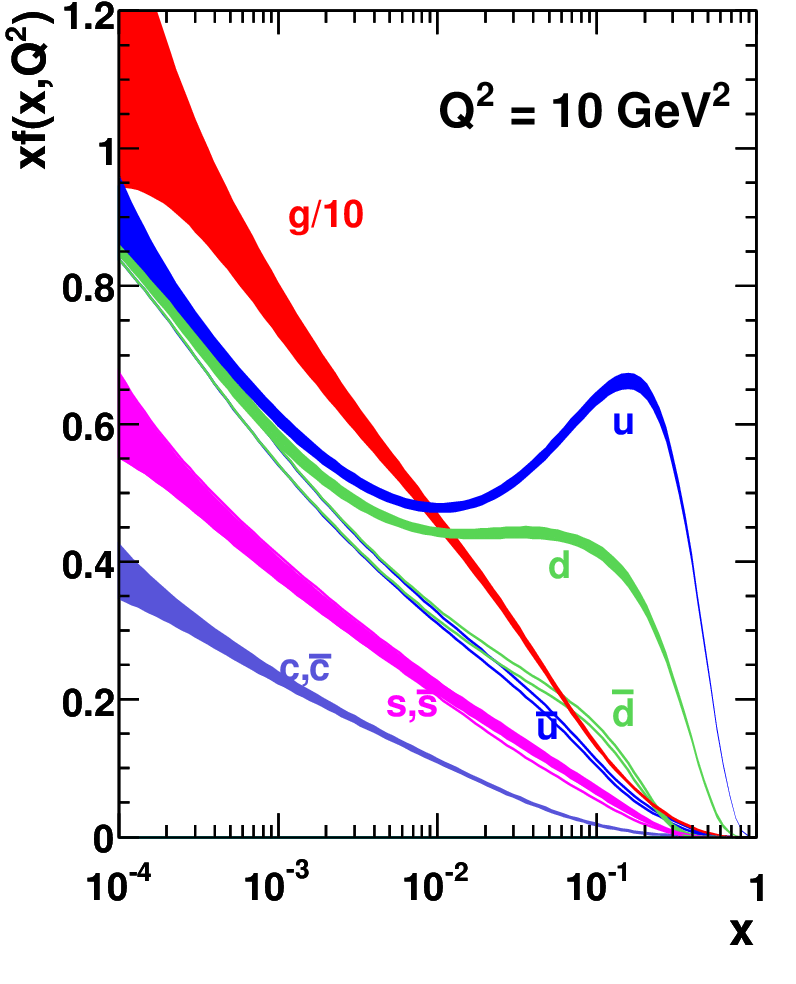
\includegraphics[width=0.5\textwidth]{figures/01-SM-03-SM/qcd/The-MSTW-2008-proton-PDFs.png}
	\caption{PDFs for the proton at $Q^2 = 10 \GeV$, reproduced from Ref.~\cite{Krasny2010}.}
	\label{fig:01_sm_qcd_pdfs}
\end{figure}

\subsubsection{The partonic cross section}

The partonic cross-section $\hat\sigma(Q^2, \mu_r)$ is an important theoretical input for measurements at high energy colliders.
The dependence on $\mu_r$ is perhaps surprising; however, it represents the fact that $\hat\sigma$ is calculated perturbatively: the $\mu_r$ dependence only appears in the highest order term of the expansion.
Indeed, this scale dependence would disappear at infinite order in perturbation theory.
While it may seem a nuisance, in fact, it provides a convenient handle to estimate the \textit{uncertainties} on our theoretical predictions by simply varying $\mu_r$ and $\mu_f$.\footnote{See Ref.~\cite{Salam:2010zt} 4.1 for further discussion.}

One important feature to keep in mind regarding the perturbative calculations for hadron colliders is that the leading order (LO) predictions are often a factor of $\gtrsim 2$ off the higher order next-to-LO (NLO) and next-to-NLO (NNLO) calculations.
This is exemplified in the predictions for \PZ boson production at the LHC, shown in Figure~\ref{fig:01_sm_qcd_qcd_nlo}.
The reason for this, despite $\alpha_s$ being reasonably small ($\approx 0.1$) at the scale for this process $m_Z \simeq 90\GeV$, is simply that the $\mathcal O(\alpha_s)$ corrections have large coefficients~\cite{Salam:2010zt}.
This is why measurements at the LHC relying on LO simulations often multiply the cross-section with an NLO / LO ``K-factor''.

Practically, matrix elements are first calculated as a function of the input and output ``hard particle'' momenta, after which event generator programs such as \MADGRAPH~\cite{Alwall:2014hca} use Monte Carlo (MC) methods to sample events appropriately from the overall phase space.
NLO and NNLO calculations are more complicated and often involve weighting events negatively to represent subtractions at higher orders~\cite{Danziger:2021xvr}.

\begin{figure}[ht]
	\centering
	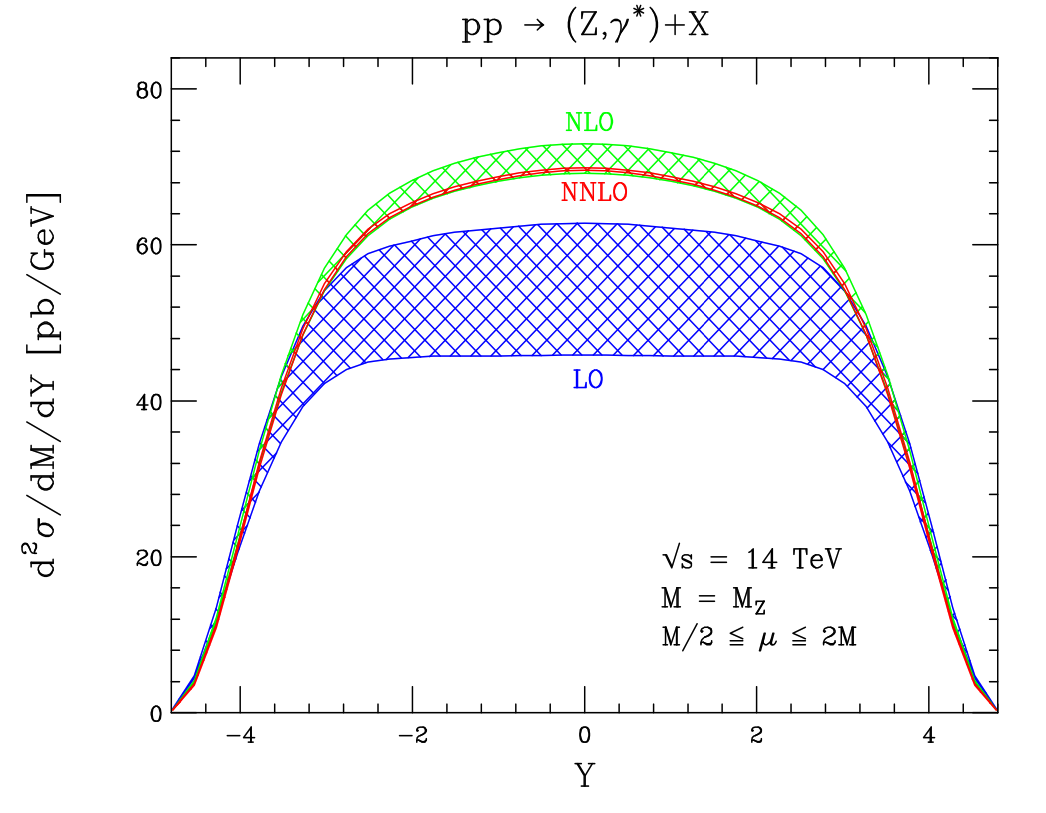
\includegraphics[width=0.7\textwidth]{figures/01-SM-03-SM/qcd/Zxs.png}
	\caption{LO, NLO, and NNLO predictions and uncertainties for $pp$ to Z boson production, differential in rapidity $Y$ at the LHC, reproduced from Ref.~\cite{Anastasiou:2003ds}.}
	\label{fig:01_sm_qcd_qcd_nlo}
\end{figure}


\subsubsection{Parton evolution}

Each parton has a certain probability of radiating another quark or gluon, with a fraction of the original parton's momentum, $z$.
These are called parton splitting functions, $P_{ij}(z)$, depicted in Figure~\ref{fig:01_sm_qcd_splitting}, and can be calculated perturbatively in QCD (see e.g. Ref.~\cite{Salam:2010zt}).
They are then further convolved with PDFs to derive their evolution with the energy scale:
\begin{equation}
	\label{eq:01_sm_qcd_pdf_evolution}
	\frac{\dd f_i(x, Q^2)}{\dd Q^2} = \frac{1}{Q^2} \sum_{j} \int_x^1 \frac{\dd z}{z} f_j(\cnicefrac{x}{z}, Q^2) P_{ji}(z).
\end{equation}

Equations~\ref{eq:01_sm_qcd_pdf_evolution} are called the Dokshitzer-Gribov-Lipatov-Altarelli-Parisi (DGLAP) evolution equations, after five physicists who developed them in the 1970s, and are analogous to the renormalization group flows of coupling constants.
The dependence of the PDFs on the energy scale has been confirmed in DIS experiments, which are then also used to fit the parameters of the PDFs, as shown in Figure~\ref{fig:01_sm_qcd_dglap}.

\begin{figure}[ht]
	\centering
	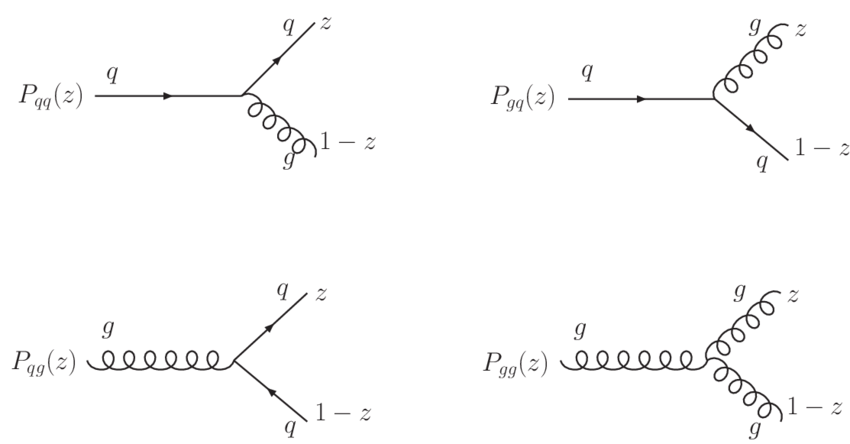
\includegraphics[width=0.9\textwidth]{figures/01-SM-03-SM/qcd/The-splitting-functions.png}
	\caption{The splitting functions for quarks and gluons, reproduced from Ref.~\cite{Kollar:2007TopQuark}.}
	\label{fig:01_sm_qcd_splitting}
\end{figure}

\begin{figure}[ht!]
	\centering
	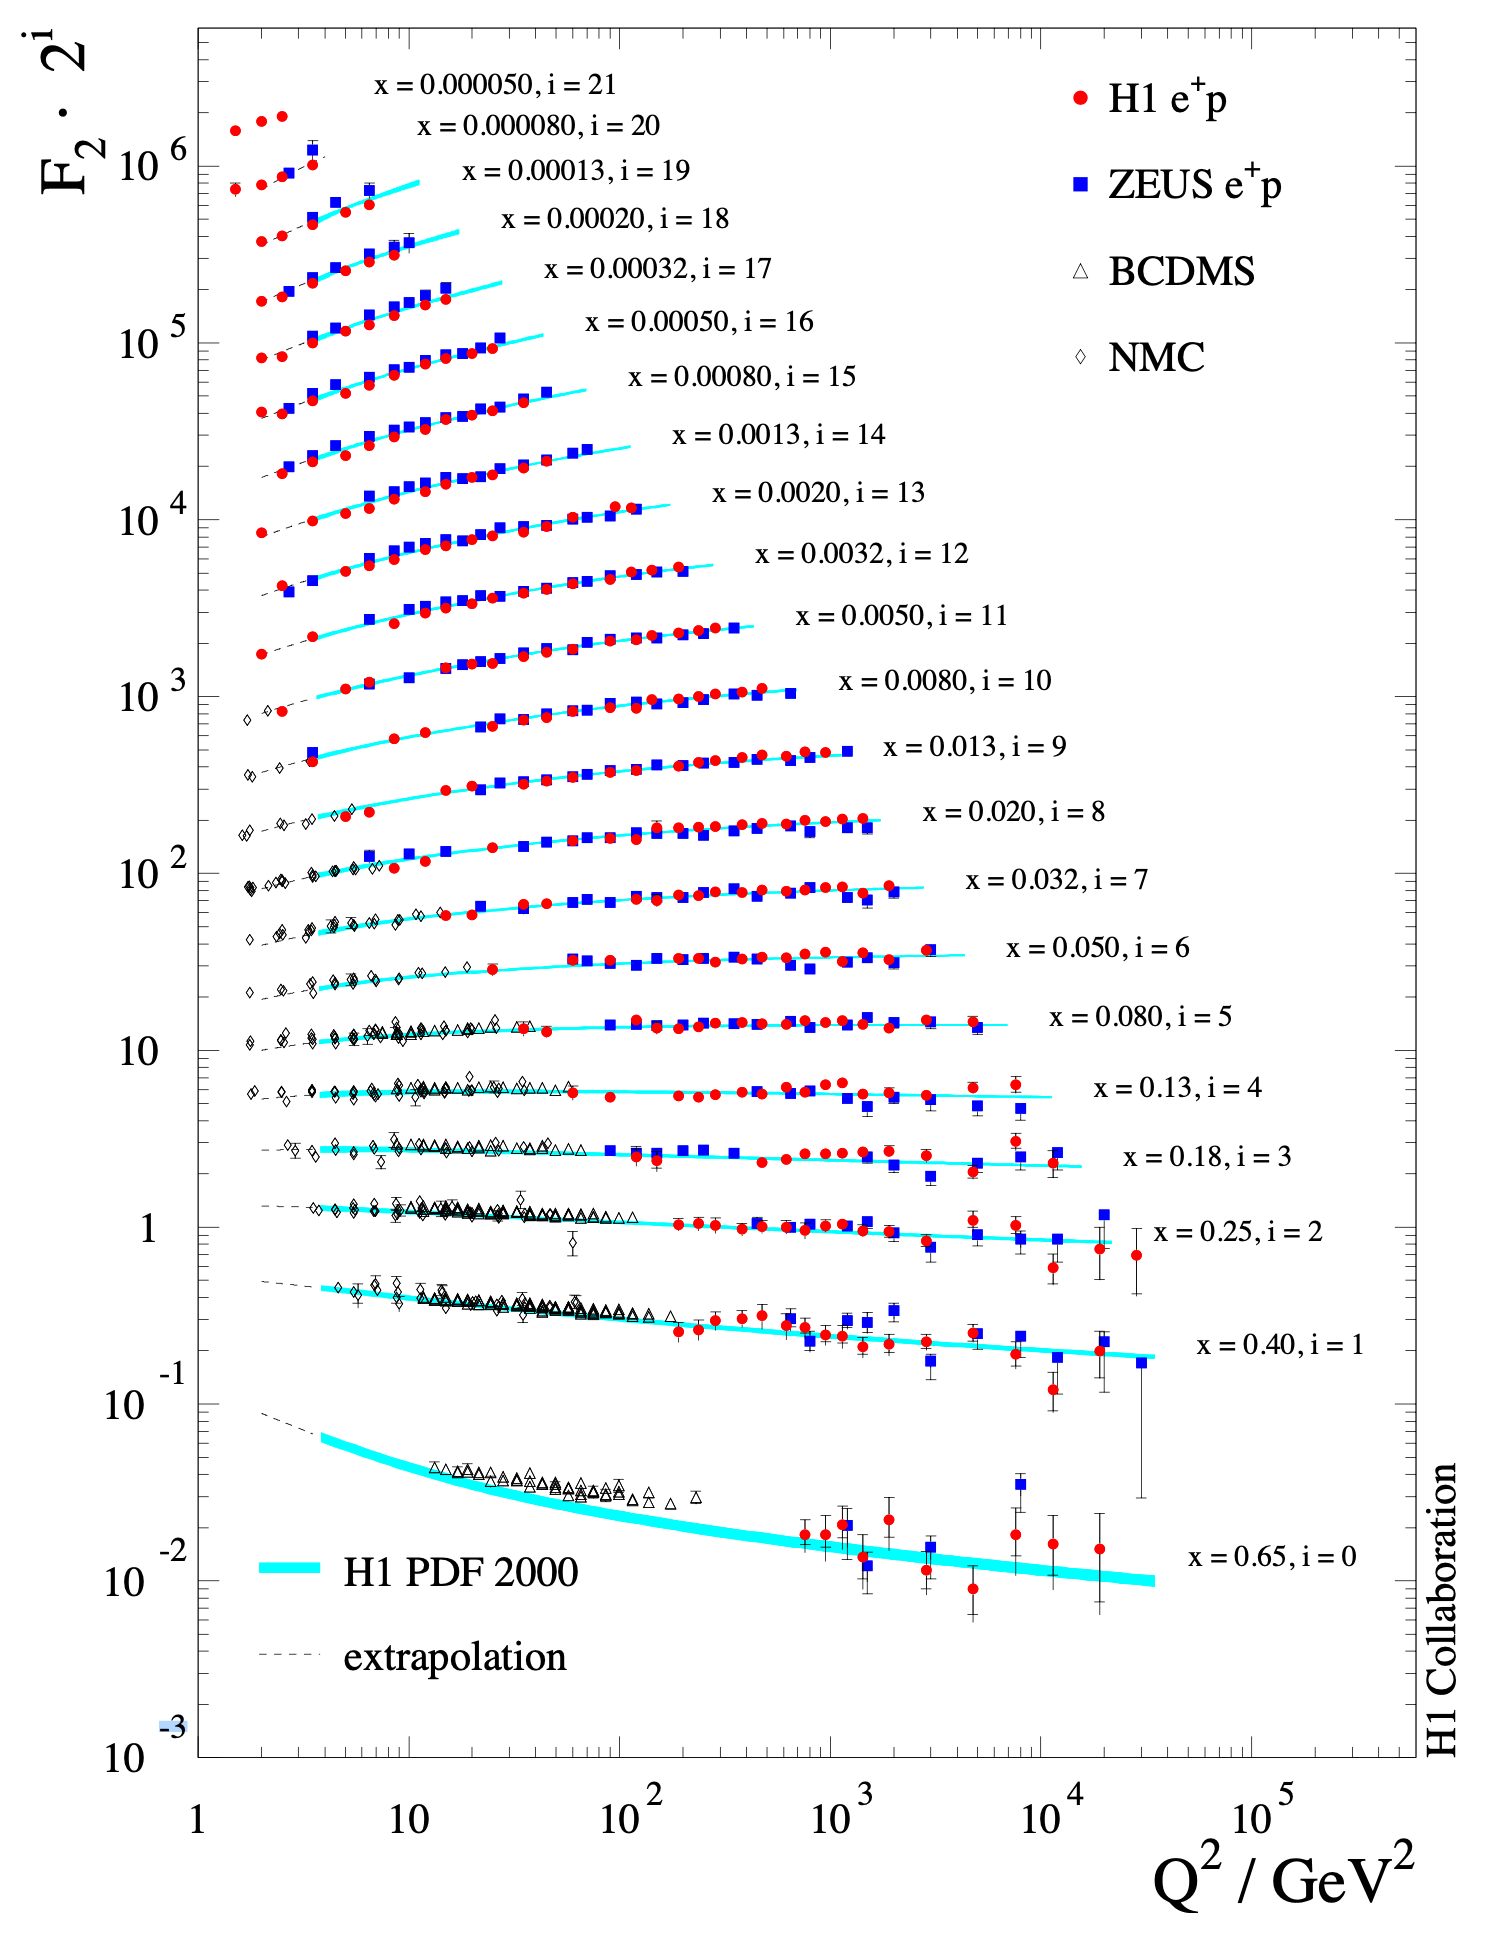
\includegraphics[width=0.75\textwidth]{figures/01-SM-03-SM/qcd/HERA_DIS.png}
	\caption{PDF measurements at different energy scales $Q^2$ and momentum fraction $x$ by the H1 collaboration in DIS experiments, reproduced from Ref.~\cite{Glazov:2007zz}.}
	\label{fig:01_sm_qcd_dglap}
\end{figure}


\subsection{Jets}
\label{sec:01_sm_qcd_jets}

As one may infer from the DGLAP equations (Eq.~\ref{eq:01_sm_qcd_pdf_evolution}), when high energy partons are produced at a collider, they will probabilistically radiate further and further partons --- called \textit{parton showering} --- until they approach the confinement scale and start forming bound hadrons --- called \textit{hadronization}.
For sufficiently high energy initial partons, the resulting hadrons will appear as a collimated spray of particles in the detector, called a \textit{jet} (Figures~\ref{fig:01_sm_qcd_jet_cartoon} and~\ref{fig:01_sm_qcd_jet_event}).

Since quarks and gluons are never observed in isolation, their production can only be inferred by understanding the jets they form.
Moreover, at a hadron collider, the high-energy hadrons continuously radiate partons \textit{before} and \textit{after} the collision as well, with the resulting jets referred to as \textit{initial} and \textit{final state radiation} (ISR and FSR), respectively.
Such jets are by far the most prevalent outputs of collisions at the LHC and, hence, represent a significant background in many measurements and searches, particularly those searching for hadronic final states.

\begin{figure}[ht]
	\centering
	\captionsetup{justification=centering}
	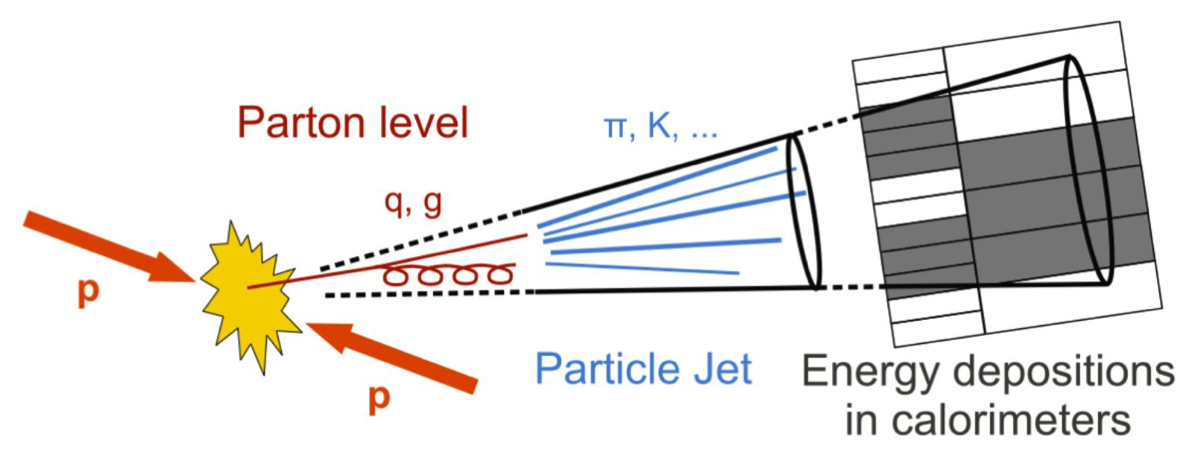
\includegraphics[width=\textwidth]{figures/01-SM-03-SM/qcd/jet_cartoon.png}
	\caption{A cartoon of a jet, reproduced from Ref.~\cite{Kirschenmann:2014vga}.}
	\label{fig:01_sm_qcd_jet_cartoon}
\end{figure}

\begin{figure}[ht]
	\centering
	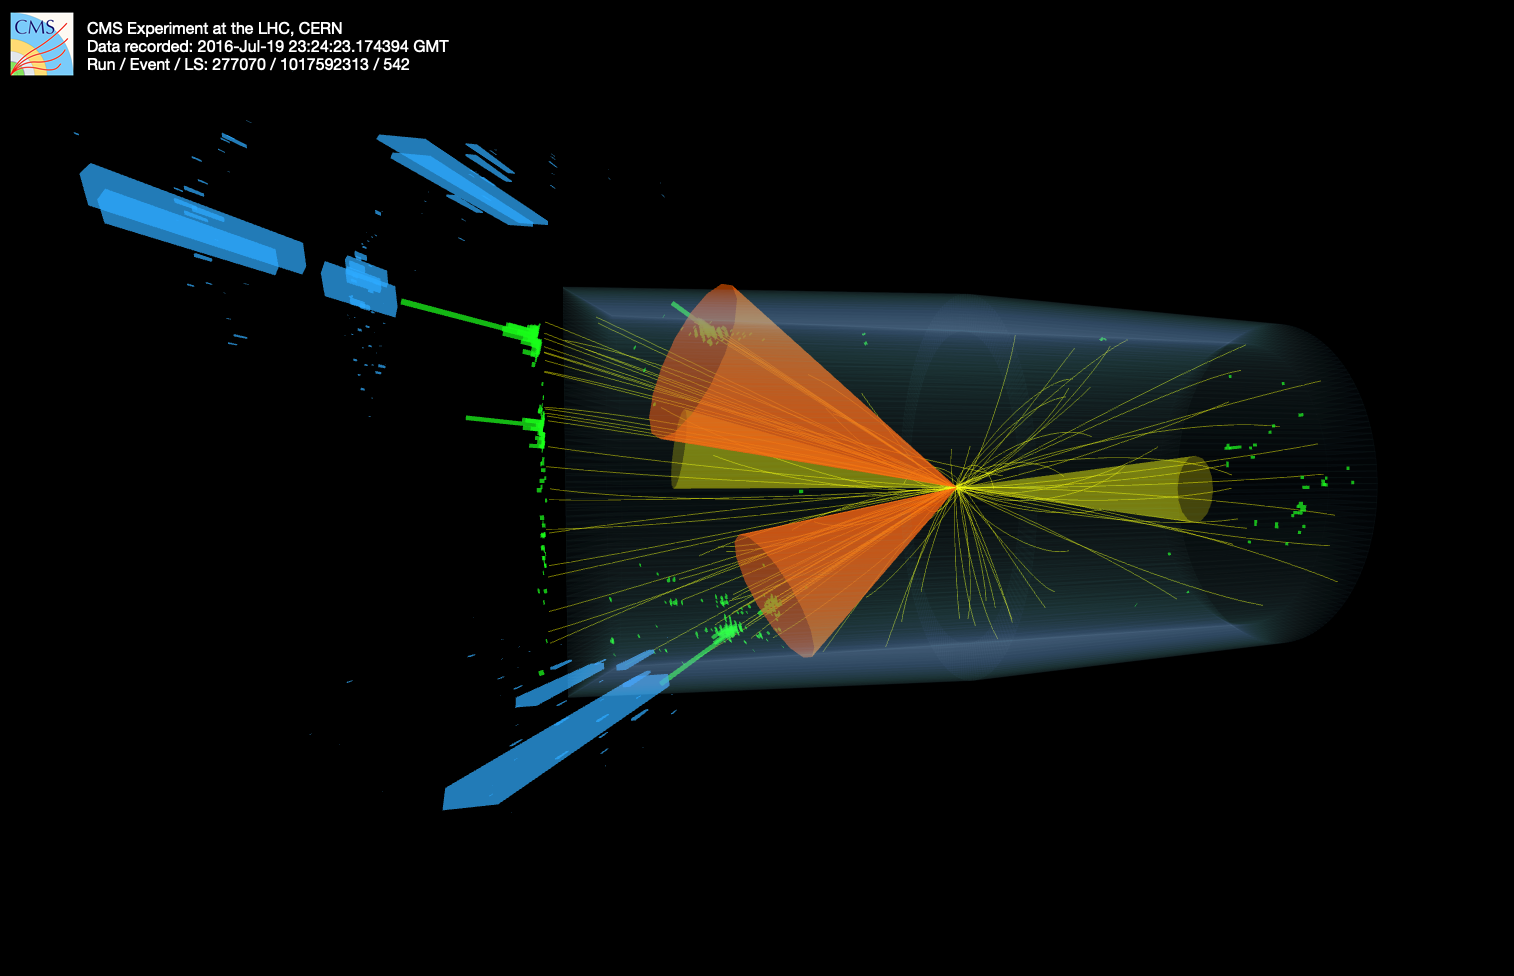
\includegraphics[width=\textwidth]{figures/01-SM-03-SM/qcd/bbww_event.png}
	\caption{An example of real jets in an event collected by CMS and identified in the search described in Chapter~\ref{sec:05_hh}~\cite{Bauerdick:2011zz, CMS:2024les}.
	An interactive version of this event display is available at \url{https://cms3d.web.cern.ch/HIG-23-012/.}}
	\label{fig:01_sm_qcd_jet_event}
\end{figure}


\subsubsection{Parton showering}

Jets can be understood and modeled by factorizing the dynamics.
As above, the parton scattering cross section (referred to as the \textit{hard process} and calculated perturbatively) is separated from the PDFs (measured from data) and their evolution (DGLAP equations).
This evolution is what produces the showering, and is modeled by numerically iterating through $Q^2$ (or, equivalently, through time) and randomly emitting new partons according to the splitting functions via MC sampling.

There are several subtleties involved in this process which numerical parton shower generators, such as \PYTHIA~\cite{Sjostrand:2014zea}, \HERWIG~\cite{Corcella:2000bw}, and \SHERPA~\cite{Sherpa:2019gpd} must account for.
First, the probability of gluon emission diverges in the soft --- i.e., low gluon energy --- and collinear --- small gluon angle with the parent parton --- limits.
Physically, this can be interpreted as the limit of our experimental resolution: at a certain point we cannot resolve two close-by or detect arbitrarily soft particles.

These are known as the \textit{infrared} and \textit{collinear} (IRC) divergences, respectively, and are typically regulated by introducing cut-off energies and angles for emissions (below which we can reasonably argue that perturbation theory is anyway invalid).
These divergences also mean that when analyzing jets in experimental data, care must be taken in defining observables to be \textit{IRC-safe}, meaning that jet clustering algorithms and physical properties derived therein should not be sensitive to arbitrarily soft or collinear emissions.

Another issue is that a naive combination of the hard matrix element and subsequent parton shower calculations may lead to double-counting of emissions, as illustrated in Figure~\ref{fig:01_sm_qcd_doublecounting}.
This necessitates a careful ``matching procedure'', such as the most common MLM scheme~\cite{Alwall:2007fs}, which defines cut-off energy and angular scales to separate the matrix element and parton shower phase spaces.
Other considerations include preserving unitarity, color coherence and color flow, and differences between ISR and FSR (see e.g. Refs.~\cite{Hoche:2014rga, Hoche:2018Lecture}).

\begin{figure}[ht]
	\centering
	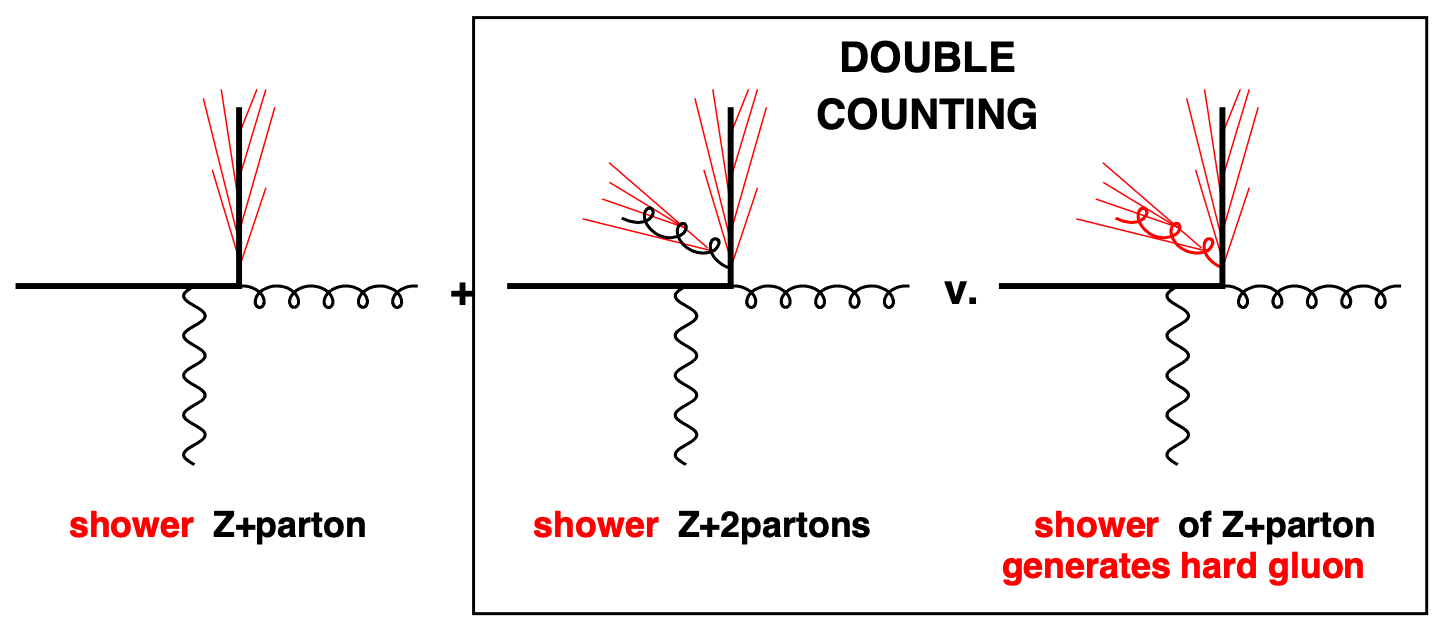
\includegraphics[width=0.8\textwidth]{figures/01-SM-03-SM/qcd/double_counting.png}
	\caption{An illustration of double-counting when combining matrix element predictions (in black) with parton showering algorithms (in red) for $Z+$parton and $Z+$2-parton events, reproduced from Ref.~\cite{Salam:2010zt}.}
	\label{fig:01_sm_qcd_doublecounting}
\end{figure}


\subsubsection{Hadronization}

The final element of the factorized process is hadronization, once the parton shower approaches the confinement scale.
This is a completely nonperturbative process and, hence, like PDFs, we must rely on numerical simulations and experimental measurements.

Lattice QCD simulations, such as those shown in Figure~\ref{fig:01_sm_qcd_fluxtubes}, indicate that in the low energy limit, the effective potential between quarks increases linearly with distance, resembling string tension:
\begin{equation}
	\label{eq:01_sm_qcd_string}
	V(r) = \sigma r,
\end{equation}
where $\sigma$ is the string tension coefficient.
In fact, this analogy can be extended further: above a certain energy, the string appears to ``snap'', in the sense that it becomes possible and energetically more favorable to produce a quark-antiquark pair.

This analogy the basis of the \textit{Lund string model} of hadronization~\cite{Andersson:1983ia}, illustrated in Figure~\ref{fig:01_sm_qcd_lundstring}.
The strong force between the final state partons is modeled as a series of strings stretched between them that probabilistically break into new partons.
Other models are based on clustering partons into color-neutral combinations~\cite{Corcella:2000bw}.

\begin{figure}[ht]
	\centering
	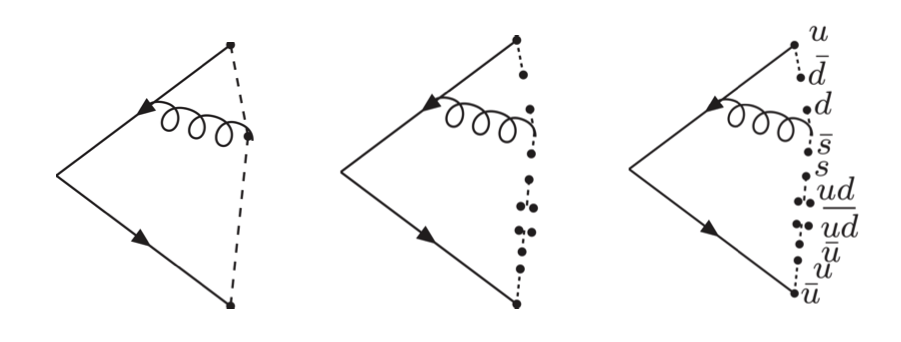
\includegraphics[width=0.6\textwidth]{figures/01-SM-03-SM/qcd/Lund_string.png}
	\caption{An illustration of the Lund string model of hadronization, reproduced from Ref.~\cite{Prestel:2018Lecture}.}
	\label{fig:01_sm_qcd_lundstring}
\end{figure}


% \subsubsection{Defining jets}

% As discussed above, it is important to define jets in an IRC-safe way.

%  - kT class of algorithms, anti-kT is most common \\

% \subsubsection{Identifying jets}

%  - jetnet cartoon \\
%  - quarks vs gluons \\
%  - ``heavy jets'', b jets \\
%  - jet substructure for boosted tops, Higgs \\

% \subsection{Chiral symmetry breaking}


\section{Electroweak interactions}
\label{sec:01_sm_ew}

The weak interaction is the last of the three fundamental forces we discuss in the SM.
Apart from its relatively weak coupling constant (Table~\ref{tab:01_sm_coupling_constants}), it is unique in several ways: (1) it couples only to left-chiral fermions, thereby violating parity ($P$) and charge conjugation ($C$); (2) it is the only force with massive gauge bosons, resulting in short-range interactions; and (3) it is the only force that ``sees'' and can change the flavors of the fermions.
Hence, it is responsible for radioactive decays and the instability of all hadrons and leptons bar the proton and electron.
Its couplings to the different flavors also lead to $CP$-violation, as we discuss in Section~\ref{sec:01_sm_ew_flavor}.

\subsection{Weak interactions}
\label{sec:01_sm_ew_weak}

The first theory of weak interactions was Enrico Fermi's 1933 theory of beta decay~\cite{Fermi:1934hr}: the decay of the neutron to a proton, $n \to p + e^- + \bar\nu_e$, through a four-fermion interaction (Figure~\ref{fig:01_sm_ew_fermi}, left).
Fermi was inspired by Dirac's nascent theory of QED, and using similar perturbative techniques, his theory proved successful in describing weak decays.
The same principle was also applied to other weak decays, such as muon decay (Figure~\ref{fig:01_sm_ew_fermi}, right) and pion decay.

As it turned out, the four-fermion interaction is of mass dimension $6$ and not renormalizable (see Chapter~\ref{sec:01_qft_interactions}), leading to the scattering cross-section diverging at high energies.
This is, of course, because these interactions are in fact mediated by the massive weak $W^\pm$ and $Z$ gauge bosons, which become relevant around their mass scale of $\mathcal O(100\GeV)$.
We now understand the Fermi theory as an effective field theory (EFT) valid for energies much lower than $100 \GeV$, wherein the $W$ and $Z$ boson DoFs can be integrated out and nonrenormalizable interactions are allowed --- they are just suppressed by factors of $(\cnicefrac{1}{M_W})^2$.
This suppression is why the weak interaction is so weak, with a coupling constant of $\approx \mathcal O(10^{-6})$ at the mass scale of the proton.

\begin{figure}[ht]
	\centering
	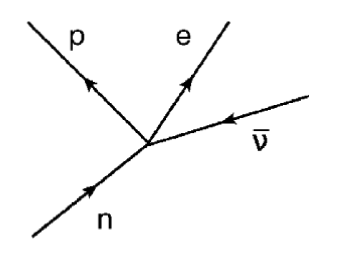
\includegraphics[width=0.25\textwidth]{figures/01-SM-03-SM/ew/beta_decay.png}
	\hspace{1cm}
	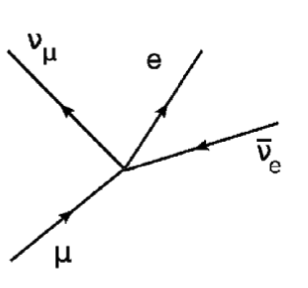
\includegraphics[width=0.2\textwidth]{figures/01-SM-03-SM/ew/muon_decay.png}
	\caption{Feynman diagrams for beta decay (left) and muon decay (right) in Fermi's theory.}
	\label{fig:01_sm_ew_fermi}
\end{figure}

% The discovery of the non-renormalizability of Fermi's theory in the 1950s led to disenchantment with QFT~\cite{WeinbergHistoryQFT}.
% with the advent of Yang-Mills theory, it was proposed that

The weak interaction is described by an \SU[2] Yang-Mills theory, and is sometimes referred to as quantum flavordynamics (QFD) because of its deep connection to flavor, as we will discuss.
However, ``vanilla'' Yang-Mills theories cannot accommodate massive gauge bosons; hence, it was only after the development of the ABEGHHK (Higgs) mechanism in the 1960s that this description gained traction.
Specifically, Sheldon Glashow, Abdus Salam, Steven Weinberg and others showed that the spontaneous breaking of an \SU[2] $\times$ \UU[1] symmetry to \UU[1] could not only yield massive weak gauge bosons, but also naturally incorporate QED with a massless photon~\cite{Glashow:1959wxa, Salam:1968rm, Weinberg:1967tq}.

This combined \textit{electroweak} theory has been experimentally confirmed in many stages:
first with the discovery of \textit{neutral currents} involving neutrinos with the Gargamelle bubble chamber at CERN in 1973~\cite{GargamelleNeutrino:1973jyy}, the first evidence for the $Z$ boson (the only neutral boson that couples to neutrinos);
then with the direct discovery of the $W$ and $Z$ bosons at the Super Proton Synchrotron (SPS) in 1983~\cite{UA1:1983crd, UA1:1983mne, UA2:1983tsx, UA2:1983mlz}, as well as precision measurements of electroweak parameters such as the $W$ and $Z$ masses with the Large Electron-Positron Collider (LEP) in the 1990s;
and finally with the discovery of the Higgs boson at the LHC in 2012~\cite{CMS:2012qbp, ATLAS:2012yve}, a particle predicted by the ABEGHHK mechanism, and the ongoing measurements of its properties.


\subsection{Before electroweak symmetry breaking}

Electroweak interactions are associated with the $\SU[2]_L \times \UU[1]_Y$ gauge symmetry, which is ``spontaneously broken'' to $\UU[1]_{\text{EM}}$ through the ABEGHHK mechanism during electroweak symmetry breaking (EWSB).\footnote{As discussed in Chapter~\ref{sec:01_qft_higgs}, technically, the gauge symmetry cannot be broken --- what breaks is the associated global symmetry.}
We label the three gauge bosons of $\SU[2]_L$ as $W^1, W^2, W^3$ and of $\UU[1]_Y$ as $B$, with coupling constants $g$ and $g'$, respectively.

The fermions in the SM can be categorized by their representations, or charges, under the three gauge symmetries before EWSB, as in Table~\ref{tab:01_sm_ew_fermions}.
The bold numbers indicate the dimension of the representation under the respective symmetry group, while the regular numbers are the charges under the $\UU[1]_Y$ group --- referred to as their \textit{hypercharge}, $Y$.

\begin{table}[ht]
	\renewcommand{\arraystretch}{1.5}
	\centering
	\caption{The representations and charges of fermionic and scalar fields in the SM under the $\UU[1]_Y$, $\SU[2]_L$, and $\SU[3]_C$ gauge symmetries.
	The right-handed neutrino is included here for completeness but has not been experimentally confirmed.}
	\begin{tabular}{c|ccc}
		\toprule
		 & $\UU[1]_Y$ & $\SU[2]_L$ & $\SU[3]_C$ \\
		\midrule
		$Q_L$ & $+ \cnicefrac{1}{6}$ & $\mathbf{2}$ & $\mathbf{3}$ \\
		$L_L$ & $- \cnicefrac{1}{2}$ & $\mathbf{2}$ & $\mathbf{1}$ \\
		$u_R$ & $+ \cnicefrac{2}{3}$ & $\mathbf{1}$ & $\mathbf{3}$ \\
		$d_R$ & $- \cnicefrac{1}{3}$ & $\mathbf{1}$ & $\mathbf{3}$ \\
		$e_R$ & $-1$ & $\mathbf{1}$ & $\mathbf{1}$ \\
		$\nu_R$? & $0$ & $\mathbf{1}$ & $\mathbf{1}$ \\
		$H$ & $+ \cnicefrac{1}{2}$ & $\mathbf{2}$ & $\mathbf{1}$ \\
		\cbottomrule
	\end{tabular}
	\label{tab:01_sm_ew_fermions}
\end{table}

The weak interactions specifically are associated with the $\SU[2]_L$ gauge symmetry, and their key characteristic is that they violate parity: they only couple to left-handed fermions and right-handed antifermions (hence, the subscript $L$).
Specifically, the left-handed quarks ($u_L$ and $d_L$) and leptons ($\nu_L$ and $e_L$) reside in $\SU[2]_L$ doublets:
\begin{equation}
	\label{eq:01_sm_ew_doublets}
	Q_L = \begin{pmatrix} u_L \\ d_L \end{pmatrix}, \quad L_L = \begin{pmatrix} \nu_L \\ e_L \end{pmatrix},
\end{equation}
while right-handed fermions live in the trivial representation.
The $L$ and $R$ subscripts indicate left- and right-chiral Weyl spinors, respectively.
Note that there are actually three generations of fermions, which we index as $u^i$ for $i = 1, 2, 3$; however, before EWSB, there is no distinction between them as they are all massless.
Often, we will omit this index when the properties across generations are identical.

The SM also contains a scalar, \SU[2]-doublet ``Higgs'' field $H$, which is listed in Table~\ref{tab:01_sm_ew_fermions} as well.
Its dynamics are governed by the Lagrangian:
\begin{equation}
	\label{eq:01_sm_ew_higgs_lagrangian}
	\mathcal{L}_{\mathrm{Higgs}} = (D_\mu H)^\dagger (D^\mu H) - \lambda (H^\dagger H - \frac{v^2}{2})^2,
\end{equation}
where $v$ is a constant and
\begin{equation}
	\label{eq:01_sm_ew_higgs_derivative}
	D_\mu H = \left[\partial_\mu - igW_\mu - \frac{i}{2} g' B_\mu\right]H
\end{equation}
is the covariant derivative of $H$.
The potential resembles the sombrero potential from Figure~\ref{fig:01_qft_higgs_potential}, but with a 2D rather than 1D complex field.

The Higgs field is able to couple to the fermions without violating gauge symmetry through Yukawa interactions.
The most general possible Yukawa terms are $3 \times 3$ matrices across the three generations.
\begin{equation}
	\label{eq:01_sm_ew_yukawa}
	\mathcal{L}_{\mathrm{Yukawa}} = -y^d_{ij} \bar{Q}^i_L H d^j_R - y^u_{ij} \bar{Q}^i_L \tilde H u^j_R - y^e_{ij} \bar{L}^i_L H e^j_R - y^\nu_{ij} \bar{L}^i_L \tilde H \nu^j_R + \text{h.c.},
\end{equation}
where $\tilde H = i\sigma_2 H^\dagger$ is the charge-conjugated Higgs field, $i$ and $j$ index the three generations of fermions, $y^d_{ij}$ are the Yukawa coupling constant matrices, and h.c. denotes the Hermitian conjugate of all the preceding terms.

The Higgs field contracts with the fermionic left-handed \SU[2]-doublets to produce an \SU[2]-singlet, while the quark fields contract with each other to form \SU[3]-singlets.
One can also check that through our clever choice of $H$ vs. $\tilde H$, the total hypercharge of each term is $0$.
Thus, each Yukawa term is independently gauge invariant.
% Finally, the quark fields contract with each other to form \SU[3]-singlets as well.

The overall electroweak Lagrangian is:
% \begin{equation}
\begin{multline}
	\label{eq:01_sm_ew_lagrangian}
	\mathcal{L}_{\mathrm{EW}} = -\frac{1}{4} W^a_{\mu\nu} W^{a\mu\nu} - \frac{1}{4} B_{\mu\nu} B^{\mu\nu} \\
	+ \bar{Q}_L i \cslashed{D} Q_L + \bar{L}_L i \cslashed{D} L_L + \bar{u}_R i \cslashed{D} u_R + \bar{d}_R i \cslashed{D} d_R + \bar{e}_R i \cslashed{D} e_R \\
	+ \mathcal{L}_{\mathrm{Higgs}} + \mathcal{L}_{\mathrm{Yukawa}},
\end{multline}
% \end{equation}
Note that without EWSB, not only are all the gauge bosons of the theory massless, but so are the fermions:
the usual fermionic mass terms of the form $m u_L u_R$ violate the $\SU[2]_L$ gauge symmetry.
% Because of this, there is also no distinction so far between the three generations of fermions.
As we will see, the ABEGHHK mechanism is what generates masses for all the fermions, through the Higgs Yukawa couplings, as well as the three weak gauge bosons.

\subsection{Electroweak symmetry breaking}
\label{sec:01_sm_ew_ewsb}

EWSB occurs when the Higgs field spontaneously breaks the global $\SU[2]_L \times \UU[1]_Y$ symmetry by moving to a ground state of the potential.
Without loss of generality, we can choose this ground state to be:
\begin{equation}
	\label{eq:01_sm_ew_higgs_vev}
	\langle H \rangle = \frac{1}{\sqrt{2}} \begin{pmatrix} 0 \\ v \end{pmatrix},
\end{equation}
where $\langle H \rangle$ is the vacuum expectation value (VEV) of the Higgs field.
As before, we can parametrize the fluctuations around this ground state as:
\begin{equation}
	\label{eq:01_sm_ew_higgs_fluctuations}
	H = e^{i \xi^A(x)T^A}
	\frac{1}{\sqrt{2}} \begin{pmatrix} 0 \\ v + h(x) \end{pmatrix},
\end{equation}
where $h$ is a real scalar field, $T^A$ are three generators of the broken $\SU[2]_L \times \UU[1]_Y$ symmetry, and $\xi^A$ are the corresponding Goldstone bosons.

The ABEGHHK mechanism for gauge theories effectively involves the original gauge bosons absorbing these Goldstone bosons, thereby acquiring mass (see Chapter~\ref{sec:01_qft_higgs}).
This can be equivalently thought of as simply a convenient choice of gauge in which $\xi^A(x) = 0$.
In the end, after some algebra, the gauge $+$ Higgs sector of the electroweak Lagrangian after EWSB looks like:
\begin{multline}
	\label{eq:01_sm_ew_gauge_lagrangian}
	\mathcal{L}_{\mathrm{GH}} = -\frac{1}{4} W^a_{\mu\nu} W^{a\mu\nu} - \frac{1}{4} B_{\mu\nu} B^{\mu\nu} + \frac{1}{2}\partial_\mu h \partial^\mu h - \underbrace{\lambda h^2 \left(v + \frac{h}{2}\right)^2}_{\equiv V(h)} \\
	+ \frac{1}{8} (v + h)^2 \left[g^2 (W^1_\mu)^2 + g^2 (W^2_\mu)^2 + (g W^3_\mu - g' B_\mu)^2\right],
\end{multline}
where $V(h)$ is the new Higgs potential.

We now have mass terms for three gauge, as well as the Higgs, bosons.
As always, we are free to define the gauge boson fields as we wish, and it turns out the most convenient choice is:
\begin{equation}
	\label{eq:01_sm_ew_gauge_fields}
	\begin{split}
		W^\pm_\mu &= \frac{1}{\sqrt{2}} (W^1_\mu \mp i W^2_\mu), \\
		Z_\mu &= \frac{1}{\sqrt{g^2 + g'^2}} (g W^3_\mu - g' B_\mu), \\
		A_\mu &= \frac{1}{\sqrt{g^2 + g'^2}} (g' W^3_\mu + g B_\mu).
	\end{split}
\end{equation}
It is conventional to define the \textit{Weinberg} or \textit{weak mixing angle} $\theta_W$:
\begin{equation}
	\label{eq:01_sm_ew_weinberg}
	\cos \theta_W = \frac{g}{\sqrt{g^2 + g'^2}}, \quad \sin \theta_W = \frac{g'}{\sqrt{g^2 + g'^2}},
\end{equation}
to simplify the forms of $Z$ and $A$ above:
\begin{equation}
	\label{eq:01_sm_ew_z_a}
	\begin{split}
		Z_\mu &= W^3_\mu \cos \theta_W - B_\mu \sin \theta_W, \\
		A_\mu &= W^3_\mu \sin \theta_W + B_\mu \cos \theta_W.
	\end{split}
\end{equation}
Experimentally, we have determined the free parameters of this theory to be:
\begin{equation}
	\label{eq:01_sm_ew_constants}
		v \approx 250\GeV, \quad \lambda \approx 0.35, \quad g \approx 0.64, \quad g' \approx 0.34 \quad \Rightarrow \quad \sin^2 \theta_W \approx 0.223,
\end{equation}
at an energy scale of the $Z$ boson mass.

The Lagrangian can hence be written as:
\begin{multline}
	\label{eq:01_sm_ew_gauge_lagrangian_weinberg}
		\mathcal{L}_{\mathrm{GH}} = -\frac{1}{4} W^+_{\mu\nu} W^{-\mu\nu} - \frac{1}{4} Z_{\mu\nu} Z^{\mu\nu} - \frac{1}{4} F_{\mu\nu} F^{\mu\nu}
		+  m_W^2 W^+_\mu W^{-\mu} + \frac{1}{2} m_Z^2 Z_\mu Z^\mu \\
		+ \frac{2 m_W^2}{v} h W^+_\mu W^{-\mu} + \frac{m_Z^2}{v} h Z_\mu Z^\mu + \frac{m_W^2}{v^2} h^2 W^+_\mu W^{-\mu} + \frac{m_Z^2}{4v^2} h^2 Z_\mu Z^\mu \\
		+ \frac{1}{2}\partial_\mu h \partial^\mu h - m_h^2 h^2 - \lambda v h^3 - \frac{1}{4} \lambda h^4,
\end{multline}
where
\begin{equation}
	\label{eq:01_sm_ew_masses}
	m_W = \frac{1}{2} vg \approx 80 \GeV, \quad m_Z = \frac{1}{2} v \sqrt{g^2 + g'^2} \approx 91 \GeV, \quad m_h = \sqrt{2\lambda} v \approx 125 \GeV.
\end{equation}

Note that in addition to the gauge-boson self-interactions, the Higgs field also has a trilinear ($\lambda v h^3$) and quartic ($\cnicefrac{1}{4} \lambda h^4$) self-interaction terms.
While some manner of EWSB has been confirmed experimentally through the discovery of the Higgs boson, its full nature, and the full form of the Higgs potential, can only be determined through measurements of these terms.
The trilinear self-coupling, in particular, can be accessed at the LHC through pair production of the Higgs boson, as we will discuss in Section~\ref{sec:01_higgs}.
Higgs pair production also allows exclusive access to the quartic $hhVV$ couplings, where $V$ is a weak gauge boson.

\subsubsection{The photon and re-emergence of Dirac spinors}

$A_\mu$ corresponds to the one unbroken symmetry of the original $\SU[2]_L \times \UU[1]_Y$ group.
In terms of the original generators --- three $T^A$s for $\SU[2]_L$ and one $Y$ for $\UU[1]_Y$ --- $A_\mu$ corresponds to linear combination $Q = T^3 + Y$.
This is the massless photon field, with the gauge group $\UU[1]_{\mathrm{EM}}$.

The eigenvalue of $Q$ for each fermion corresponds to their electric charge under this group.
For the $\SU[2]_L$-singlet fields, $T_3$ has no value and hence $Q = Y$, while for the doublets, $T_3$ has eigenvalues $\pm \cnicefrac{1}{2}$ for the upper and lower components, respectively: e.g. for $u_L$, $Q = \cnicefrac{1}{2} + \cnicefrac{1}{6} = \cnicefrac{2}{3}$ and for $e_L$, $Q = -\cnicefrac{1}{2}-\cnicefrac{1}{2} = 1$.
In the end, we see that the left- and right-chiral fermion field pairs have the same charge under this remaining unbroken symmetry, so they can again form Dirac spinors:
\begin{equation}
	\label{eq:01_sm_ew_dirac}
	\psi_u = \begin{pmatrix} u_L \\ u_R \end{pmatrix}, \quad \psi_d = \begin{pmatrix} d_L \\ d_R \end{pmatrix}, \quad \psi_e = \begin{pmatrix} e_L \\ e_R \end{pmatrix}, \quad \psi_\nu = \begin{pmatrix} \nu_L \\ \nu_R \end{pmatrix},
\end{equation}
times three for each generation.

Each Weyl spinor pair interacts identically with the photon and gluons but the $W$ and $Z$ bosons continue to couple only to the left-handed components.
For example the $W^+$--fermion coupling is:
\begin{equation}
	\label{eq:01_sm_ew_w_coupling}
	\mathcal{L}_{W^+f} = -\frac{g}{\sqrt{2}} W^+_\mu \underbrace{\left(\bar{u}_L \bar\sigma^\mu d_L + \bar{\nu}_L \bar\sigma^\mu e_L\right)}_{\equiv J^+_\mu},
\end{equation}
where $J^+_\mu$ is called the weak charged current.
%  (this interaction is hence also referred to as a weak charged current interaction).
In terms of Dirac spinors, this can be written using the projection operator (Eq.~\ref{eq:01_qft_spinors_chiral_projection}):
\begin{equation}
	\label{eq:01_sm_ew_w_coupling_dirac}
	\mathcal{L}_{W^+f} = -\frac{g}{\sqrt{8}} W^+_\mu \left(\bar{\psi}_u \gamma^\mu (1 - \gamma_5) \psi_d + \bar{\psi}_\nu \gamma^\mu (1 - \gamma_5) \psi_e\right).
\end{equation}
Recall that $\bar\psi \gamma^\mu \psi$ is a Lorentz vector, while $\bar\psi \gamma^\mu \gamma_5 \psi$ is a pseudo- or axial-vector, so the weak current is effectively an axial vector subtracted from a vector.
Indeed, historically, the weak interaction was referred to as ``V-A'' theory.

\subsubsection{A hierarchy problem}

Generally, if we encounter a new energy scale in nature, we are either able to connect it in some way to an existing scale or a (broken) symmetry of the theory.
For example, the mass of the proton $\sim 1\GeV$ is based on the QCD confinement scale $\Lambda_{\text{QCD}} \sim 200\MeV$, which in turn is related to the Planck scale $\Lambda_{\text{Planck}} \sim 10^{19}\GeV$ through dimensional transmutation.
The mass of the pion on the other hand, $\approx 140\MeV$, is a consequence of chiral symmetry breaking in QCD.
Physicists such as Dirac and Gell-Mann have in fact proposed these criteria as a principle of ``naturalness'' for physical theories~\cite{Dirac:1938mt, Gell-Mann:1956iqa}.

There are many examples of mysterious energy scales appearing experimentally, which were either later rationalized or in fact even used to correctly predict new physics, such as the prediction of the charm quark mass based on the small mass difference between the $K_L^0$ and $K_S^0$ mesons.
The electroweak energy scale of $\approx 100\GeV$ is one such example which has yet to be explained.

A common way of expressing the problem is based on the Higgs mass: if we believe the SM to be an EFT valid up to some energy scale $\Lambda$, and if we have \textit{a priori} no other energy scale to which to tie the Higgs mass, then we expect higher order corrections to its bare mass to be of order $\Lambda$.
For example, if there is no new physics up to the Planck scale, then we are left with a bare mass and correction both of order $10^{19} \GeV$.
The fact that the actual mass is $125 \GeV$ implies a cancellation between the two, or \textit{finetuning}, at a $\cnicefrac{125}{10^{19}} \approx 10^{-15}\%$ level.
This is considered highly ``unnatural'' and is called a \textit{hierarchy problem}, perhaps hinting at new physics.

One possibility is that $\Lambda$ is in fact on the order of the Higgs mass, and we are simply yet to find the new degrees of freedom at this $\mathcal O(100\GeV)$ scale.
Or, if we accept a higher level of finetuning, e.g. at the $10\%$ or $1\%$ levels, $\Lambda$ can be pushed up further to $1$--$10\TeV$.
Effectively, we can invert the hierarchy problem into setting a bound on new physics!

Another solution is the existence an underlying (approximate) symmetry of nature ``protecting'' the Higgs mass from higher order corrections, similar to the chiral symmetry for the pion mass.
The most promising candidate is \textit{supersymmetry}, postulating an additional global symmetry between bosons and fermions~\cite{Wess:1992cp}.
Both these solutions possibly hint at an extended scalar sector, with either another Higgs doublet or new scalar singlets, for example, through the minimal supersymmetric extension of the SM (MSSM)~\cite{Craig:2013hca} or based on two-real-scalar-singlet models~\cite{Robens:2019kga}.
This is one motivation behind the search for new Higgs bosons described in this dissertation.
% The fact that we have found no hints for either explanation to the hierarchy problem at the LHC in 10 years, however, has raised concerns regarding whether it is a problem at all, and not simply a fact of nature (AKA the anthropic principle)~\cite{Weinberg:1987dv}.
A more detailed, pedagogical discussion of naturalness can be found in e.g. Nathaniel Craig's IAS lectures~\cite{Craig:2017Lecture}.


\subsection{Fermion masses and flavor}
\label{sec:01_sm_ew_flavor}

After EWSB, we have
\begin{equation}
	\label{eq:01_sm_ew_higgs_tilde}
	H = \frac{1}{\sqrt{2}} \begin{pmatrix} 0 \\ v + h \end{pmatrix}, \quad
	\tilde H = \frac{1}{\sqrt{2}} \begin{pmatrix} v + h \\ 0 \end{pmatrix},
\end{equation}
which yields the following Yukawa Lagrangian:
\begin{equation}
	\label{eq:01_sm_ew_yukawa_after}
		\mathcal{L}_{\mathrm{Yukawa}} = -\frac{1}{\sqrt{2}}(v + h) \left[y^d_{ij} \bar d^i_L d^j_R + y^u_{ij} \bar u^i_L u^j_R + y^e_{ij} \bar e^i_L e^j_R + y^\nu_{ij} \bar \nu^i_L \nu^j_R\right] + \text{h.c.}.
\end{equation}
Again, we are free to redefine fields and can choose a basis for all the fermion fields in which the Yukawa matrices are diagonal:
\begin{equation}
	\label{eq:01_sm_ew_yukawa_transformation}
	u^i_L \rightarrow (V^u)^i_j u^j_L, \quad d^i_L \rightarrow (V^d)^i_j d^j_L, \quad u^i_R \rightarrow (U^u)^i_j u^j_R, \quad d^i_R \rightarrow (U^d)^i_j d^j_R,
\end{equation}
such that
\begin{equation}
	\label{eq:01_sm_ew_yukawa_diagonal}
	V^{\dagger u} Y^u U^u = \mathrm{diag}(m_u, m_c, m_t), \quad V^{\dagger d} Y^d U^d = \text{diag}(m_d, m_s, m_b),
\end{equation}
and same for the leptons (though again with the caveat that the right-handed neutrino, $\nu_R$, has not been experimentally confirmed).

This is the \textit{mass eigenstate} basis, where each generation and type of fermion has terms of the form:
\begin{equation}
	\label{eq:01_sm_ew_yukawa_mass}
	\mathcal{L}_{\mathrm{Yukawa}} = -\frac{v}{\sqrt{2}} y^u \bar u_L u_R - \frac{h}{\sqrt{2}} y^u u_L u_R + \text{h.c.} + \ldots,
\end{equation}
i.e., a mass term $m_X = \frac{v y^X}{\sqrt{2}}$ and a Yukawa interaction term with the Higgs field of strength $y^X$.
The same Yukawa constant determines both the mass of the particle and its coupling to the Higgs field;
indeed, in Appendix~\ref{sec:01_qft_spinors_feynman}, we show how this is used to determine the Higgs to fermion decay rates!

Like $v$ and $\lambda$, the Yukawa couplings are all free parameters of the SM which can only be determined experimentally.

\subsubsection{The CKM and PMNS matrices}

Observe that the transformation we needed to diagonalize the Yukawa matrices in Eq.~\ref{eq:01_sm_ew_yukawa_transformation} violates the $\SU[2]_L$ symmetry, by transforming the up and down components of $Q_L$ and $L_L$ independently.
This is actually okay because the $\SU[2]_L$ symmetry was already broken through EWSB; however, crucially, this means the weak eigenstates (also called the \textit{flavor eigenstates}), which the W bosons couple together, are not the same as the mass eigenstates!

Explicitly, any term which couples the up or down components of the \SU[2]-doublet only with their respective right-handed components, such as the kinetic terms $\partial_\mu u_L \partial^\mu u_L$ or the electromagnetic interaction $A_\mu \bar \psi_u \gamma^\mu \psi_L$, is invariant under the transformation in Eq.~\ref{eq:01_sm_ew_yukawa_transformation}.
It is only the weak charged currents (Eq.~\ref{eq:01_sm_ew_w_coupling}) in the SM which mix the two.
Including the three generations, the positive current is:
\begin{equation}
	\label{eq:01_sm_ew_flavor_jmu}
	J^+_\mu = \sum_i \bar u^i_L \bar \sigma^\mu d^i_L + \sum_i \bar \nu^i_L \bar \sigma^\mu e^i_L
\end{equation}
in the flavor eigenstate basis (the negative current is simply the h.c.).
But if we attempt to transform to the mass basis via Eq.~\ref{eq:01_sm_ew_yukawa_transformation}:
\begin{equation}
	\label{eq:01_sm_ew_flavor_jmu_ckm}
	J^+_\mu = \sum_i \bar u^i_L \bar \sigma^\mu \underbrace{[(V^u)^\dagger V^d]_{ij}}_{\equiv V_{\mathrm{CKM}}} d^j_L + \sum_i \bar \nu^i_L \bar \sigma^\mu \underbrace{[(V^\nu)^\dagger V^e]_{ij}}_{\equiv V_{\mathrm{PMNS}}} e^i_L,
\end{equation}
we are left with these two matrices, called the \textit{Cabibbo-Kobayashi-Maskawa} (CKM)~\cite{Kobayashi:1973fv} and \textit{Pontecorvo-Maki-Nakagawa-Sakata} (PMNS)~\cite{Maki:1962mu} matrices mixing the quark and lepton flavors, respectively.
The upshot is that the $W$ bosons can not only mix the components of (the former) $\SU[2]_L$ doublets, but also different mass eigenstates!
The $Z$ and photon currents do not have this property, which is why we say there are no \textit{flavor-changing neutral currents} (FCNCs) in the SM, at least at tree level.

The magnitude of this mixing by the $W$s is determined by the CKM and PMNS matrices.
They are $3 \times 3$ unitary matrices that, after accounting for the various constraints imposed by the fermion masses, unitarity, etc., have $4$ free parameters each.
They are most often parametrized as three real Euler angles and one complex phase, which again have to be determined experimentally.
Importantly, this complex phase means the weak interaction violates $CP$-symmetry as well!

To see why, we can go back to the Yukawa interactions, this time with the hermitian conjugates included:
\begin{equation}
	\label{eq:01_sm_ew_yukawa_hermitian}
	\mathcal{L}_{\mathrm{Yukawa}} \sim y^d_{ij} \bar d^i_L d^j_R + y^{d*}_{ij} \bar d^i_R d^j_L + \ldots
\end{equation}
One can check that the two field terms $\bar d^i_L d^j_R$ and $\bar d^i_R d^j_L$ are $CP$-conjugates of each other, which means invariance under $CP$ requires $y^d_{ij} = y^{d*}_{ij}$, i.e. the Yukawa matrix to be real.
The complex phases in the CKM and PMNS matrices therefore lead to $CP$-violation in the SM.
Interestingly, for fewer than three generations, the two matrices cannot be imaginary.
Kobayashi and Maskawa discovered this in 1973, after the observation of $CP$-violation in 1964, and predicted a third generation of quarks to explain $CP$-violation in the SM, for which they were awarded the Nobel prize in 2008.

Flavor is perhaps the least understood area of the SM:
Why are their exactly three generations each of quarks and leptons?
Why their particular hierarchy of masses?
Is it a coincidence that nature chose the exact minimum number of generations needed to allow for $CP$-violation?
All of these mysteries point to the strong possibility of new physics in the flavor sector.


\section{The Higgs sector}
\label{sec:01_higgs}

The Higgs boson, being the only scalar in the SM and uncharged under the $\UU[1]_{\mathrm{EM}}$ and $\SU[3]_C$ symmetries, may appear to be the simplest particle in the theory.
However, these same properties also mean that the Higgs sector is not as strongly constrained by gauge invariance, renormalizability, etc. as the gauge and fermionic sectors.
Indeed, the Higgs sector contains the majority of the free parameters of the SM: the Yukawa couplings (12 masses of the fermions $+$ 8 more parameters from the CKM and PMNS matrices), the Higgs VEV, and the Higgs mass (or, equivalently, $\lambda$ in the Higgs potential).
Without it, the SM would only have three free parameters: the three forces' coupling constants!

This is why a significant motivation for the next decades of the LHC, as well as future ``Higgs factory'' colliders, is to precisely characterize the Higgs sector.
In this section, we first describe how this is possible at the LHC and discuss recent experimental constraints.
We then motivate measurements of Higgs pair production, both in the SM and through BSM decays of heavy resonances, which are the focus of this dissertation and a key target of the current and upcoming LHC physics program.

% We then briefly motivate measurements and searches of Higgs pair production, which are the focus of this dissertation.
% % We then focus on the Higgs self- and \HHVV-quartic couplings, two key interactions which have not been well-constrained.
% % Finally, we note that the Higgs sector, being perhaps the least understood part of the SM, has a high potential to contain BSM physics and describe strategies to search for it.


\subsection{Higgs boson production and measurements at the LHC}

Higgs bosons are produced at the LHC through a variety of parton-parton interactions, as shown in Figure~\ref{fig:01_sm_higgs_production}.
Because of their high mass, they have a lifetime of roughly $\mathcal O(10^{-22})$s and decay immediately into two vector bosons or two fermions at tree-level, with further decays possible through loops.
The decay probability depends on the strength of the respective interactions, which we see from Section~\ref{sec:01_sm_ew} are proportional to the mass or the mass squared for fermions and vector bosons, respectively, though with the probability lowered for decays that are not kinematically accessible (i.e., when the total mass of the decay products is greater than the Higgs').

This is illustrated in Figure~\ref{fig:01_sm_higgs_hbrs}, which shows the branching fractions (BFs) of the Higgs boson as a function of its mass.
Generally, we see the higher the mass of the decay product, the higher the BF; however, as the Higgs mass decreases, first the \ttbar and later the $W$ and $Z$ boson decays become kinematically inaccessible, leading to decreasing decay probabilities.

\begin{figure}[ht]
	\centering
	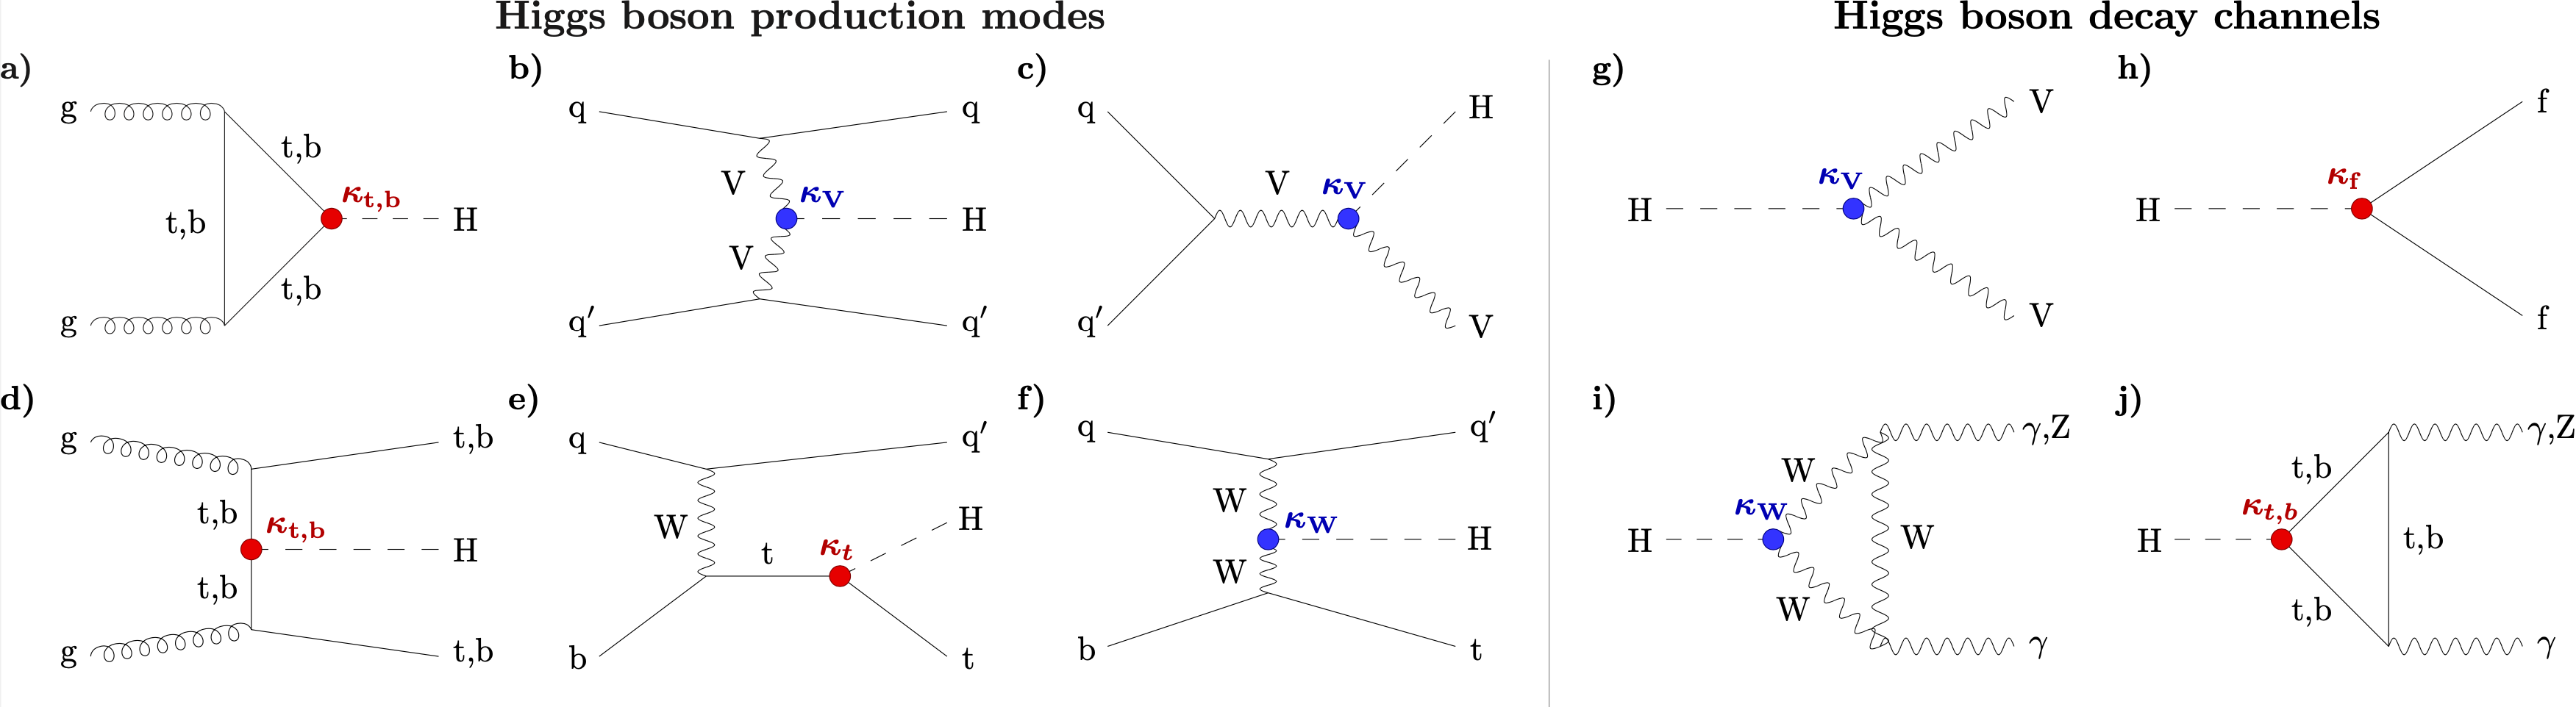
\includegraphics[width=\textwidth]{figures/01-SM-03-SM/higgs/higgs_production.png}
	\caption{Single Higgs boson production modes and decay channels at the LHC, reproduced from Ref.~\cite{CMS:2022dwd}.}
	\label{fig:01_sm_higgs_production}
\end{figure}

\begin{figure}[ht]
	\centering
	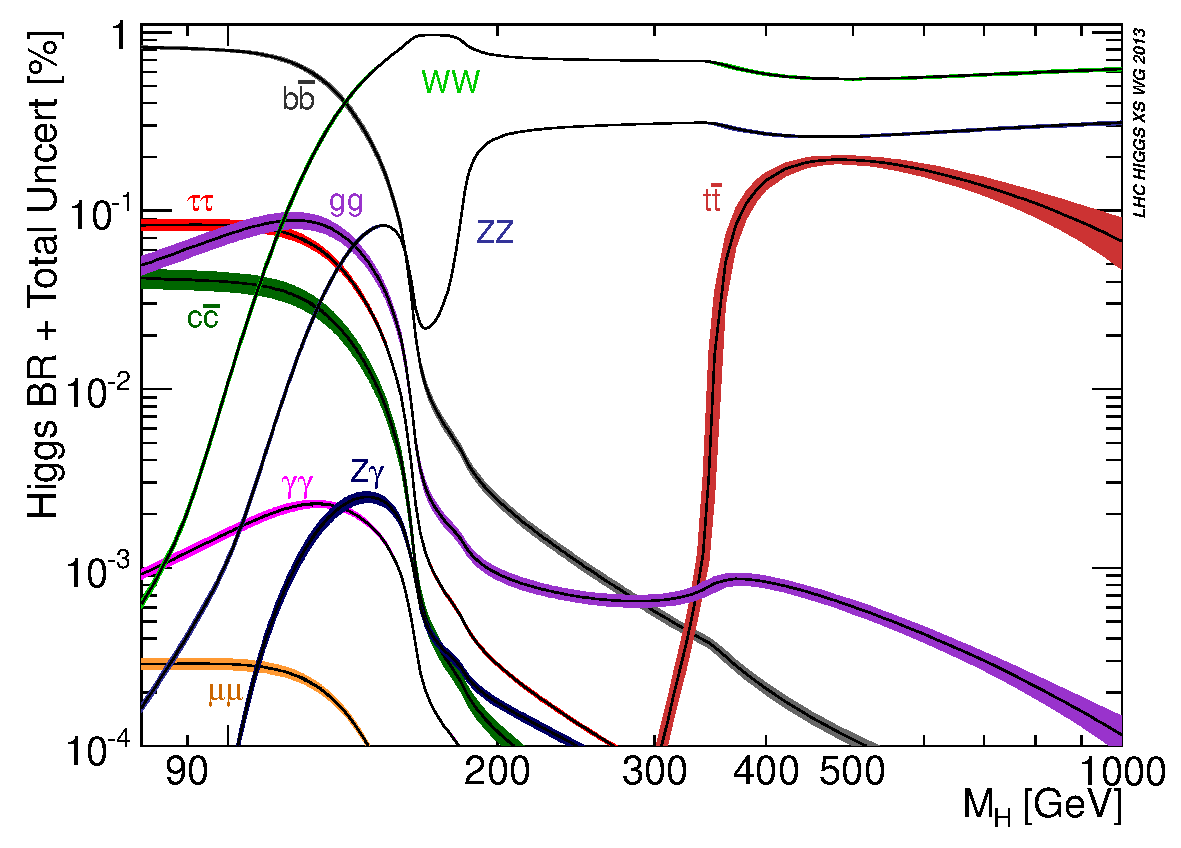
\includegraphics[width=0.8\textwidth]{figures/01-SM-03-SM/higgs/Higgs_BR_RECT.pdf}
	\caption{Higgs branching fractions predicted in the SM as a function of \mh (reproduced from Refs.~\cite{Dittmaier:2012vm,LHCHiggsCrossSectionWorkingGroup:2016ypw}).}
	\label{fig:01_sm_higgs_hbrs}
\end{figure}

The Higgs boson was initially observed by the CMS and ATLAS experiments in 2012 through a combination of several decay channels.
Since then, the two experiments have been making steady progress in the precise measurements of the various Higgs properties.
For example, Figure~\ref{fig:01_sm_higgs_constraints} shows the overall constraints on the Higgs to fermion and vector boson couplings and the Higgs mass by the CMS experiment.
Constraints are based on the $\kappa$-framework~\cite{LHCHiggsCrossSectionWorkingGroup:2013rie}, where $\kappa_X$ scales the Higgs-$X$ coupling strength with $\kappa_X = 1$ corresponding to the SM prediction.
Changes to the coupling strength due to new physics are thus generically captured by deviations from $\kappa_X = 1$.


\begin{figure}[ht]
	\centering
	\adjustbox{valign=m}{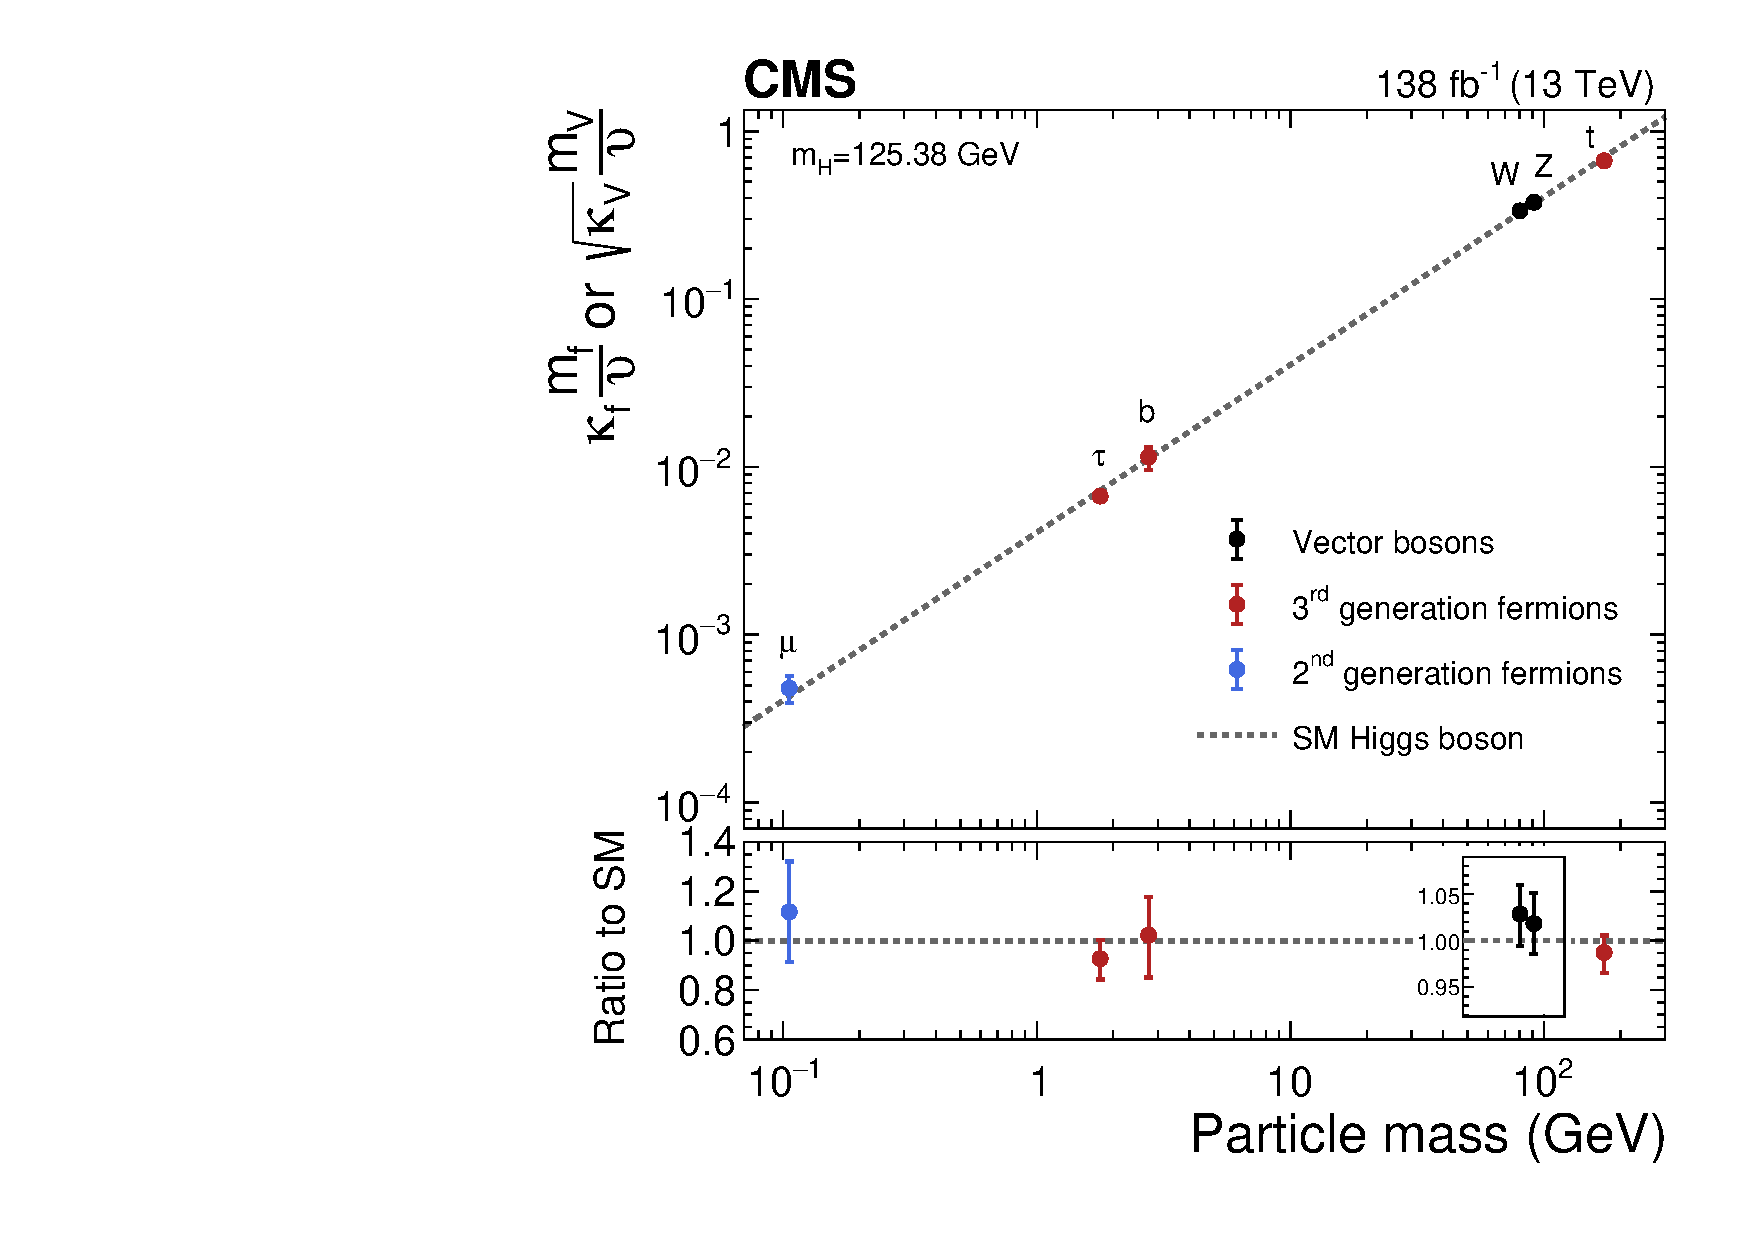
\includegraphics[width=0.49\textwidth]{figures/01-SM-03-SM/higgs/higgs_couplings.pdf}}
	\adjustbox{valign=m}{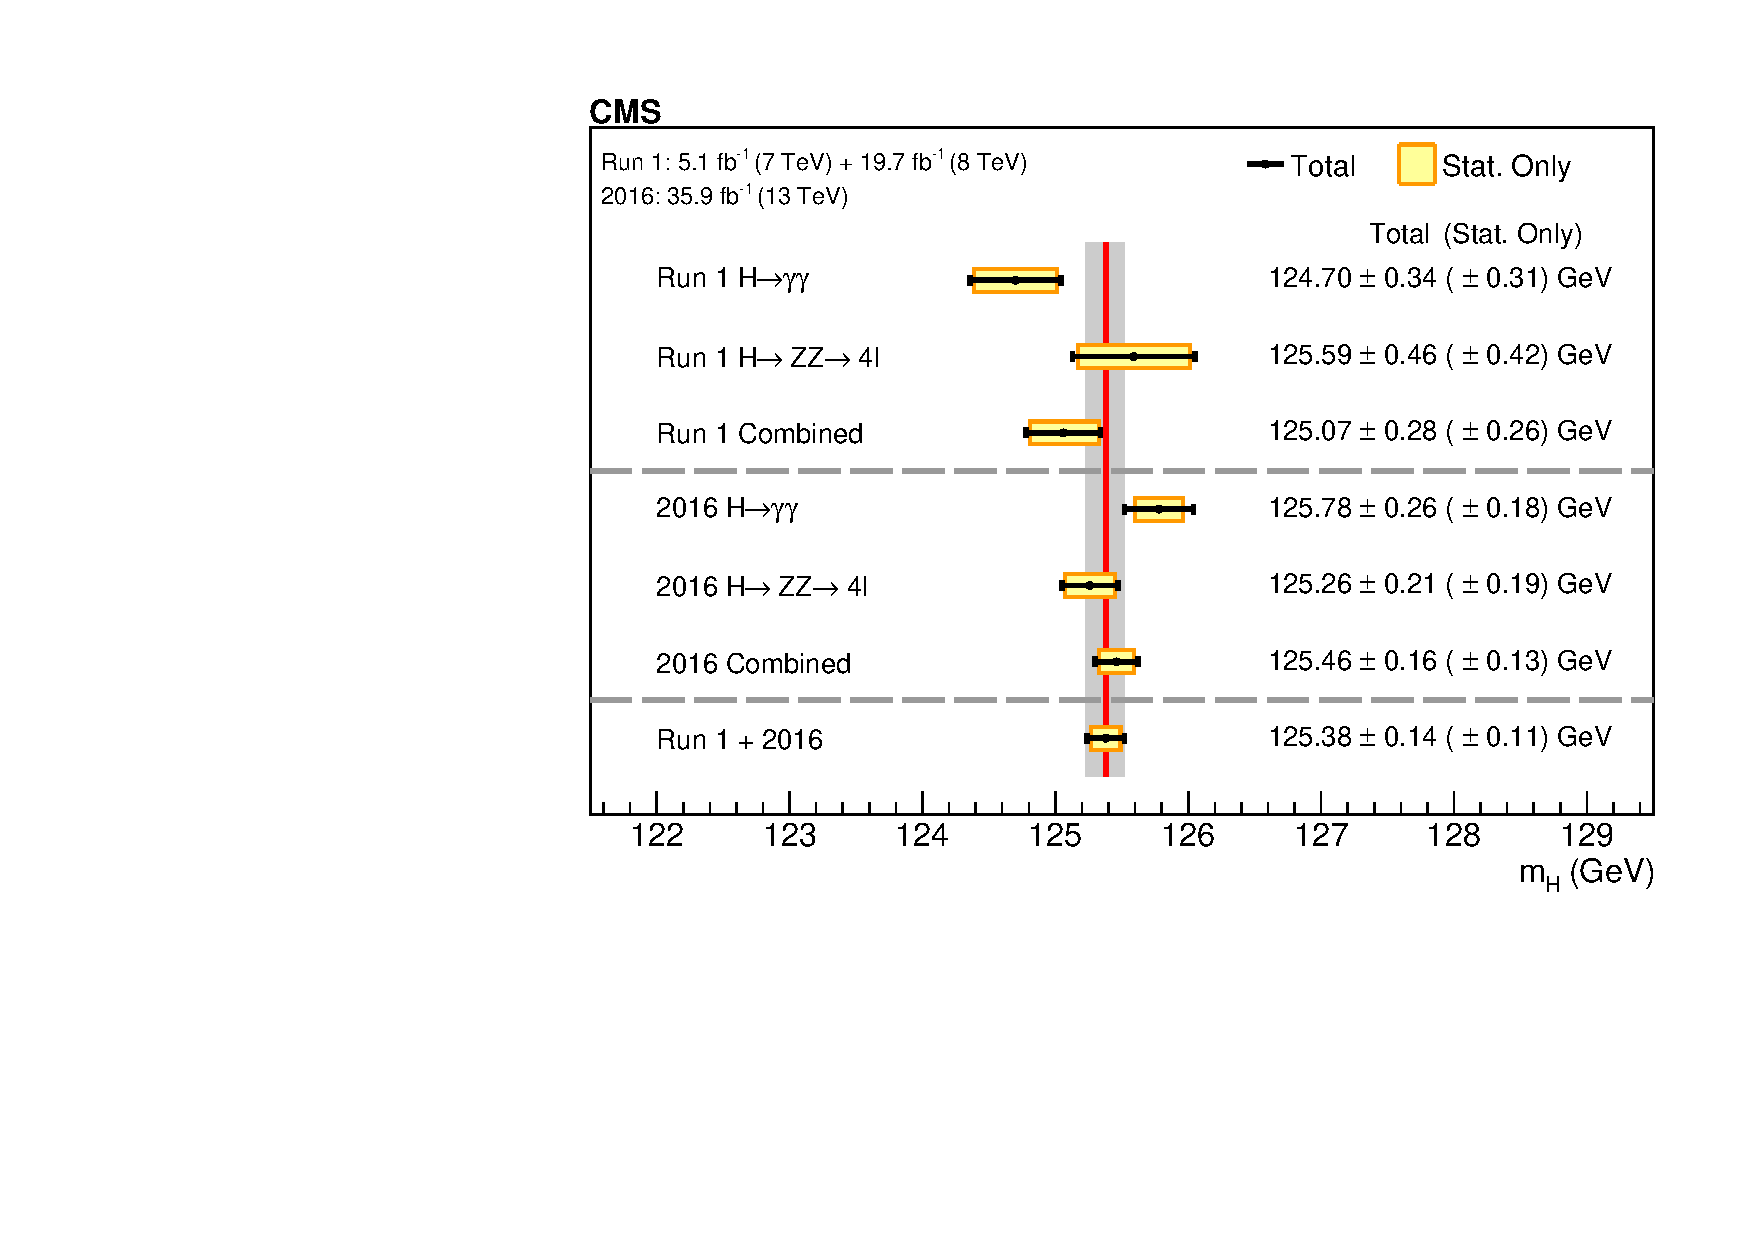
\includegraphics[width=0.49\textwidth]{figures/01-SM-03-SM/higgs/higgs_mass.pdf}}
	\caption{Constraints on Higgs to fermion and vector boson couplings, reproduced from Ref.~\cite{CMS:2022dwd} (left) and measurements of the Higgs mass, reproduced from Ref.~\cite{CMS:2020xrn} (right) by the CMS experiment.}
	\label{fig:01_sm_higgs_constraints}
\end{figure}


\subsection{Higgs pair production in the SM}
\label{sec:05_smhh}

Two couplings of the Higgs boson which have not been well-constrained are the trilinear Higgs self-coupling (\HHH), with coupling modifier \kapl, and the Higgs quartic coupling to vector bosons (\HHVV), with modifier $\kapvv$.
As discussed in Section~\ref{sec:01_sm_ew_ewsb} and illustrated in Figure~\ref{fig:01_sm_higgs_potential}, measuring the Higgs self-coupling in particular is necessary to fully characterize the Higgs potential, deviations to which could hint at BSM explanations to mysteries such as baryon asymmetry~\cite{Reichert:2017puo}.
As we describe below, both couplings can be probed exclusively through Higgs pair production (\HH), which is why it is a key physics target for the upcoming high-luminosity era of the LHC.

\begin{figure}[ht]
	\centering
	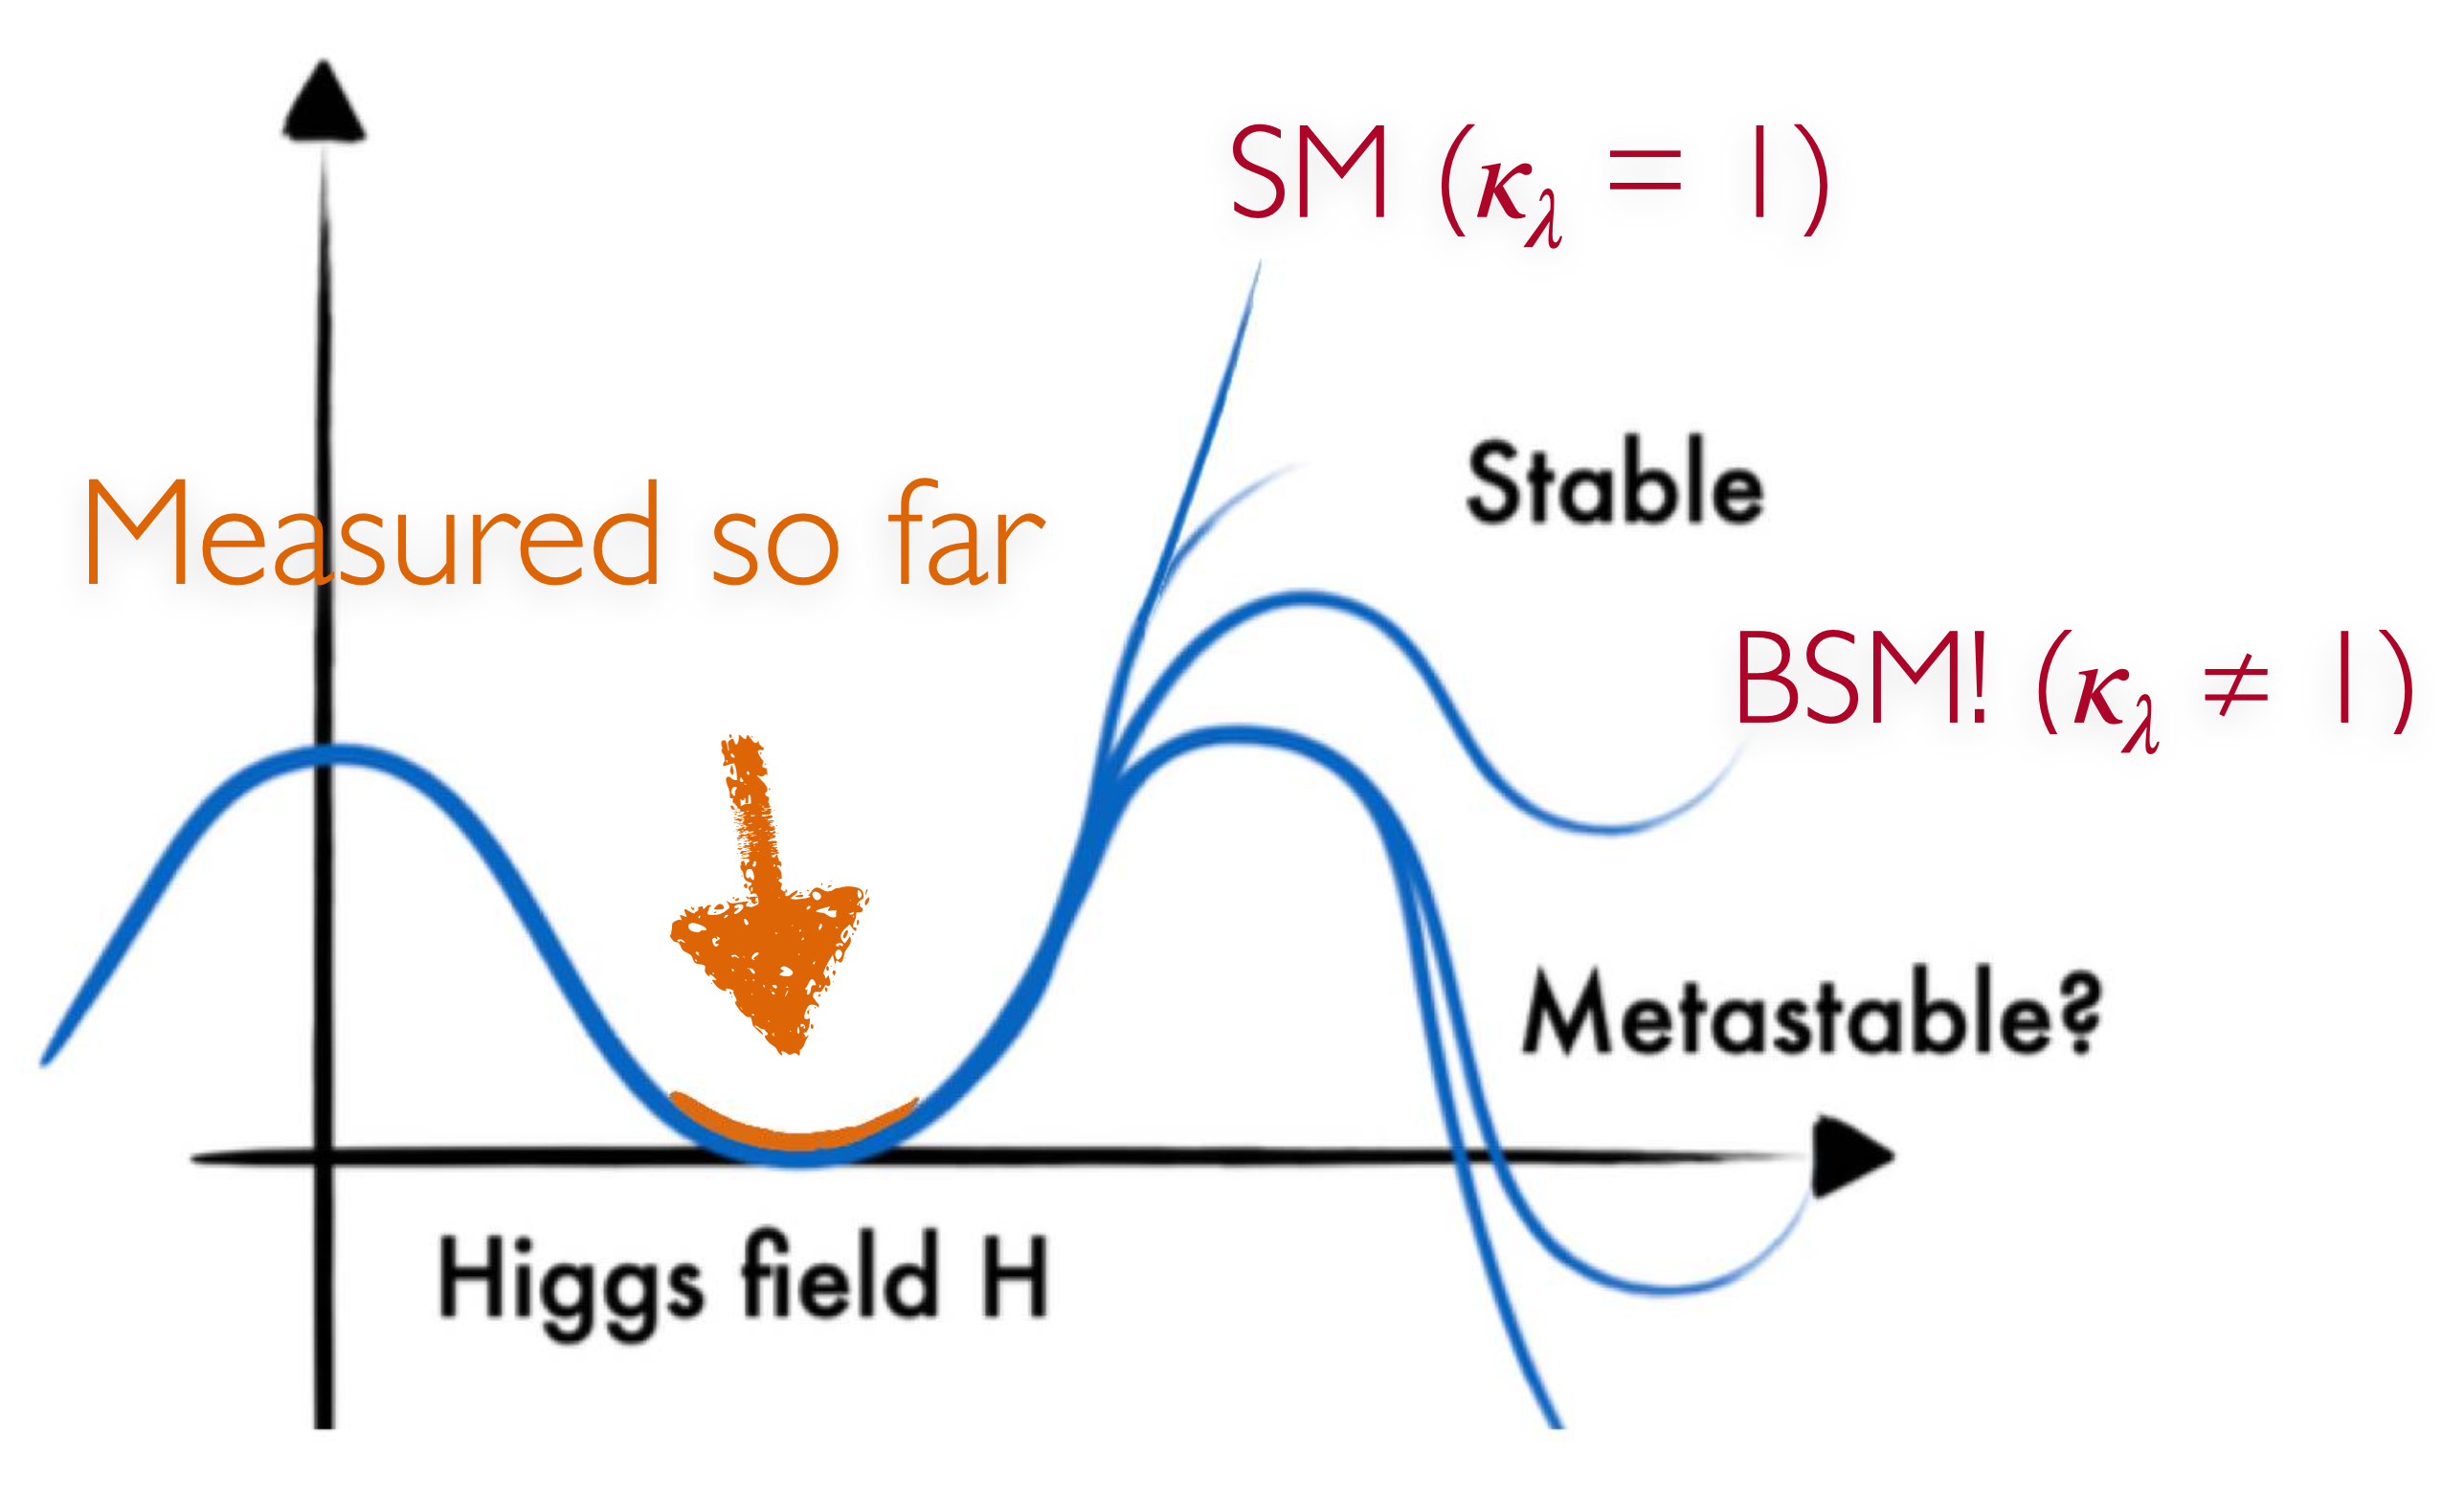
\includegraphics[width=0.5\textwidth]{figures/01-SM-03-SM/higgs/higgs_potential}
	\caption{Cartoon of the Higgs potential in the SM and potential deviations due to BSM physics.}
	\label{fig:01_sm_higgs_potential}
\end{figure}

\HH production in the SM occurs dominantly through gluon fusion (ggF), with a small production cross section $\sigma_{\mathrm{ggF}} = 31.05^{+2.2\%}_{-5.0\%} \pm 3\% (\textrm{PDF}+\alpS)^{+4\%}_{-18\%} (m_\PQt)\unit{fb}$~\cite{Grazzini:2018bsd,Baglio:2020wgt} at a center of mass energy of 13\TeV and $\mH = 125\GeV$, and subdominantly through vector boson fusion (VBF), with a smaller production cross section $\sigma_{\mathrm{VBF}} = 1.726^{+0.03\%}_{-0.04\%} \pm 2.1\% (\textrm{PDF}+\alpS)\unit{fb}$~\cite{LHCHiggsCrossSectionWorkingGroup:2016ypw}.
At leading order, the ggF production mode has contributions from diagrams that involve the trilinear \HHH Higgs self-coupling and the emission of two Higgs bosons through a top quark loop, while the VBF production mode has contributions from three diagrams involving the trilinear \HHH, \HVV, and quartic \HHVV couplings (Figures~\ref{fig:05_feynmanggf} and~\ref{fig:05_feynmanvbf}).
It also features the distinct final state signature of two, typically forward, jets in addition to the two Higgs bosons.

\begin{figure}[htb] %[ht]
    \centering
    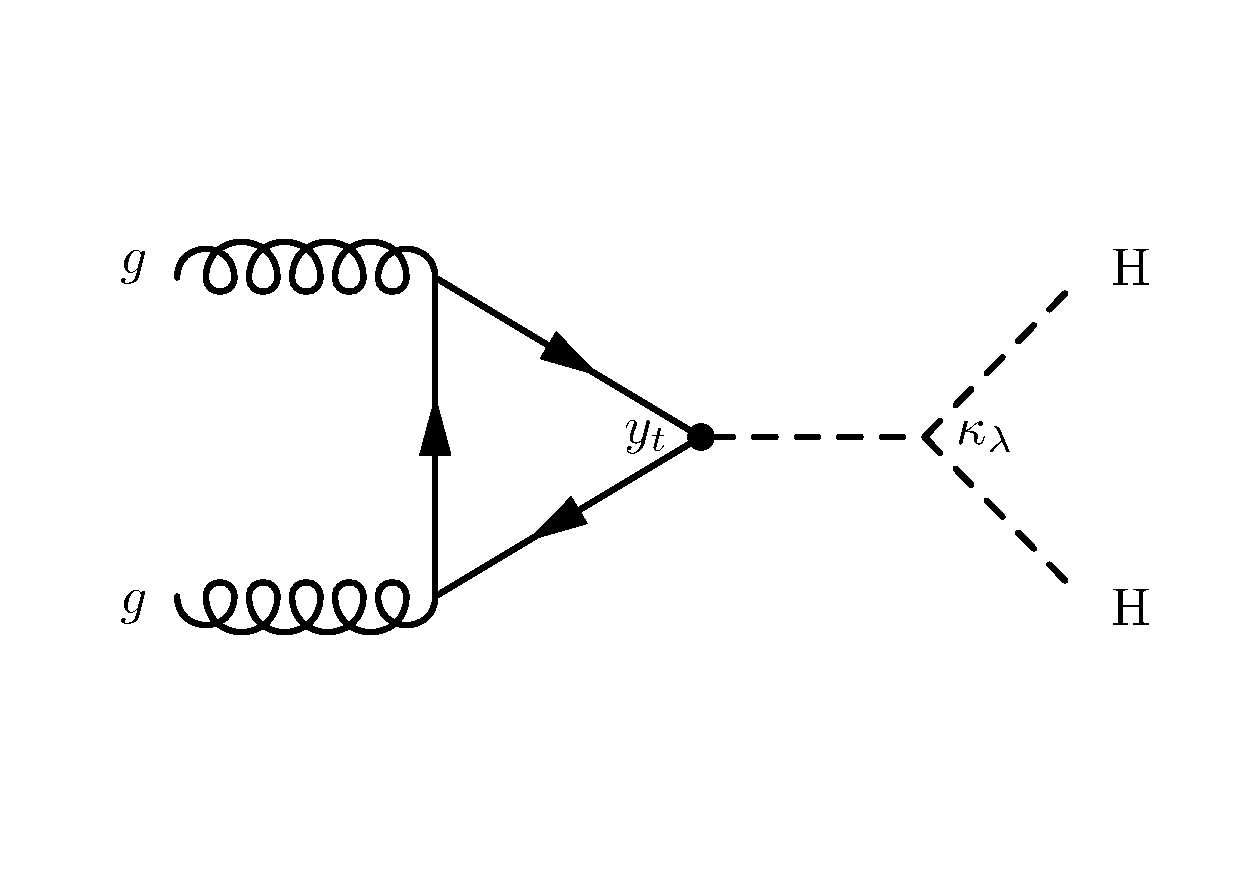
\includegraphics[width=0.4\textwidth]{figures/05-HH/production/diagrams/feynman_02.pdf}
    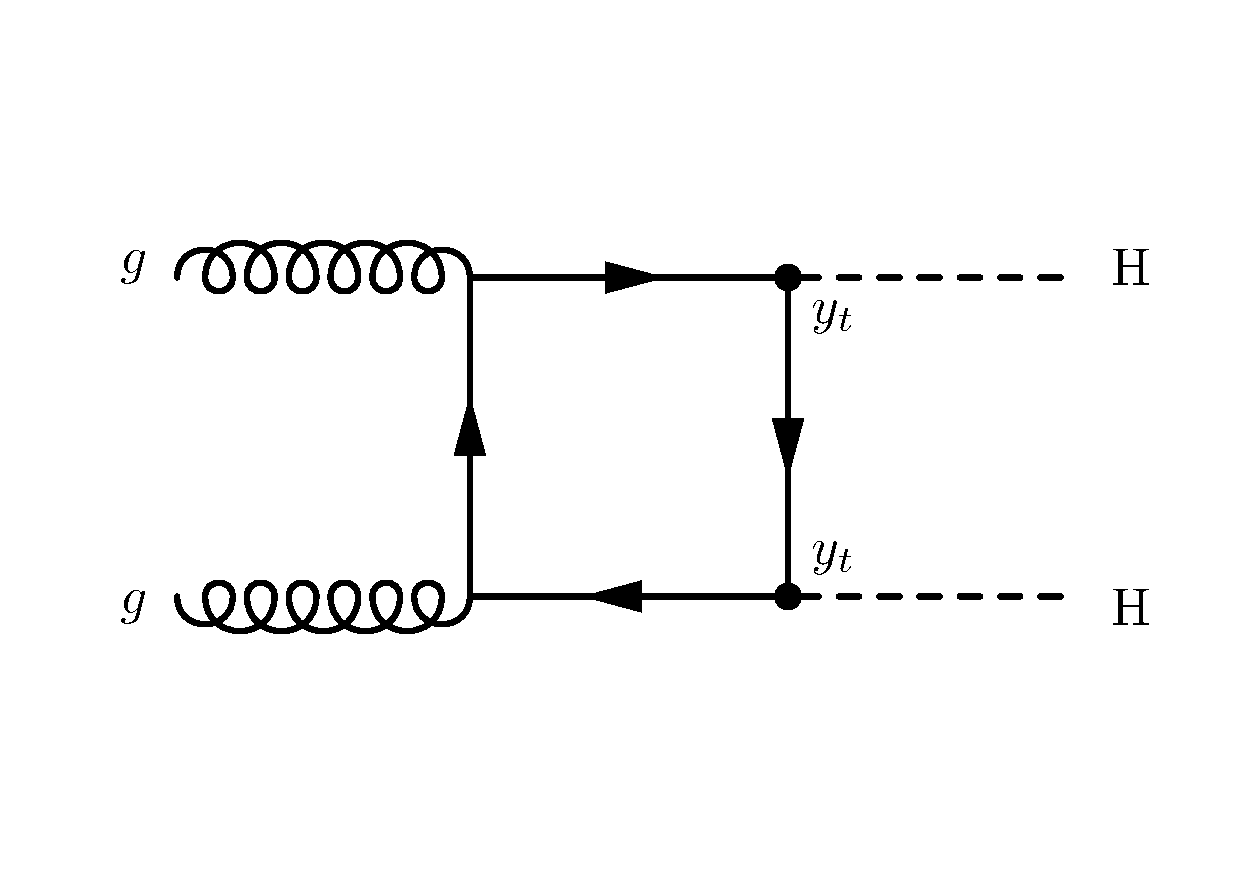
\includegraphics[width=0.4\textwidth]{figures/05-HH/production/diagrams/feynman_01.pdf}
    \caption{Leading-order diagrams for nonresonant \HH production via gluon gluon fusion.}
    \label{fig:05_feynmanggf}
\end{figure}

\begin{figure}[htb]
    \centering
    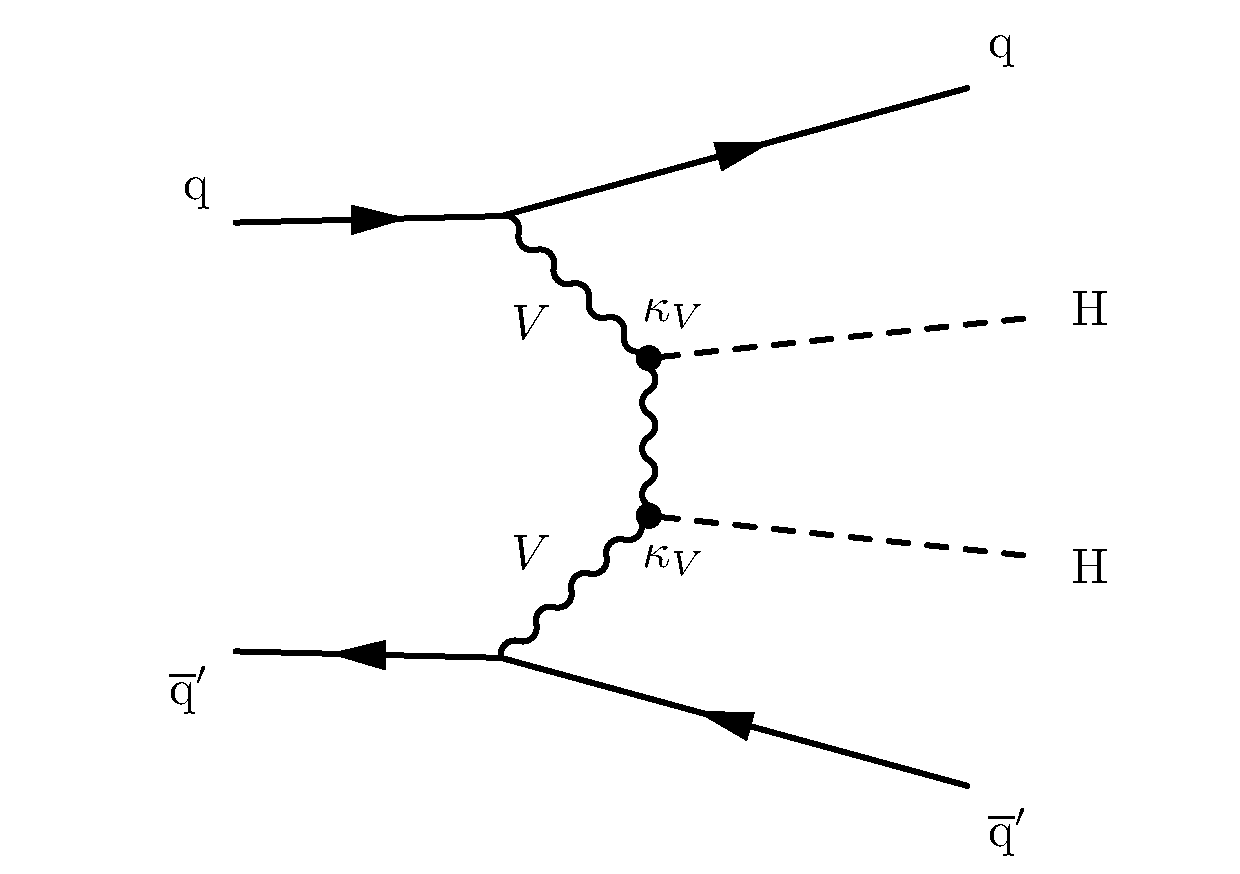
\includegraphics[width=0.32\textwidth]{figures/05-HH/production/diagrams/feynman_04.pdf}
    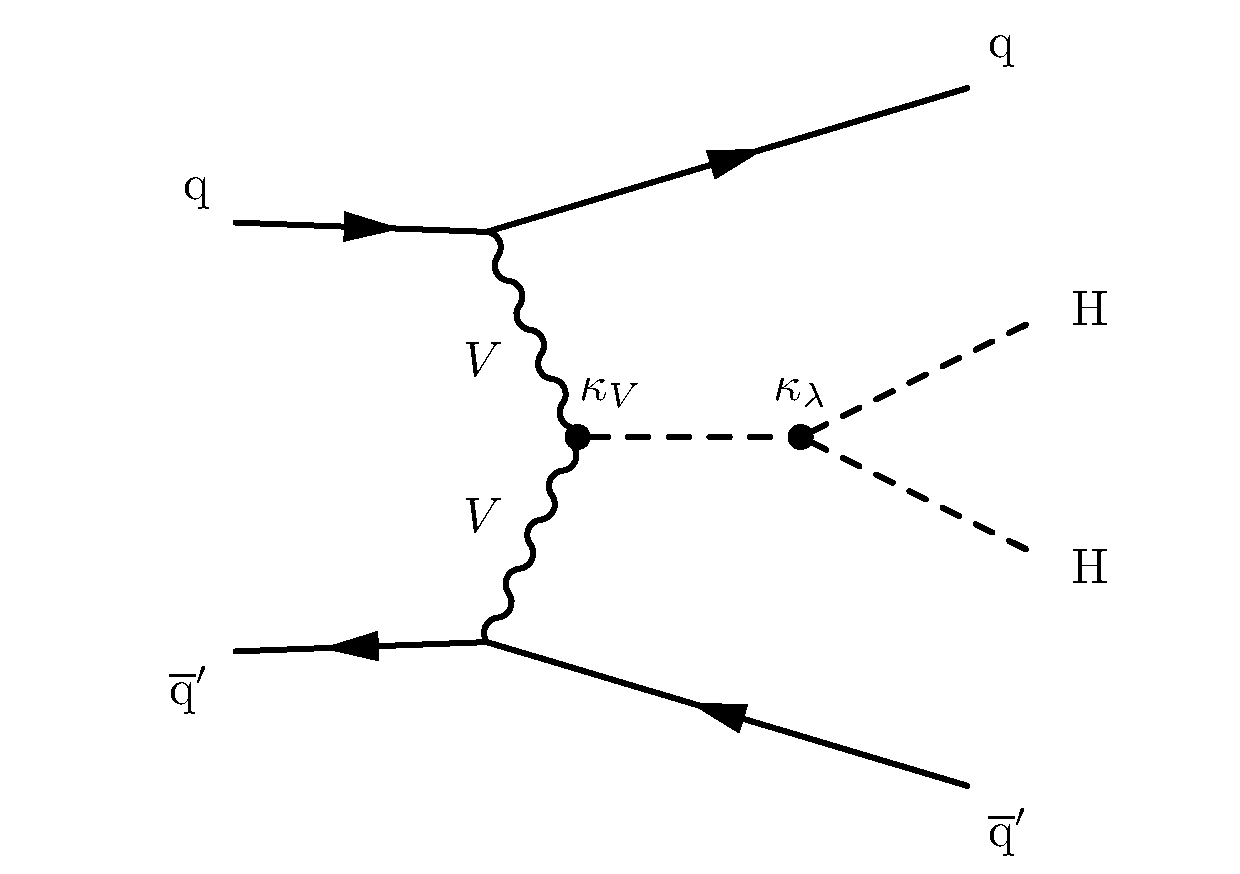
\includegraphics[width=0.32\textwidth]{figures/05-HH/production/diagrams/feynman_05.pdf}
    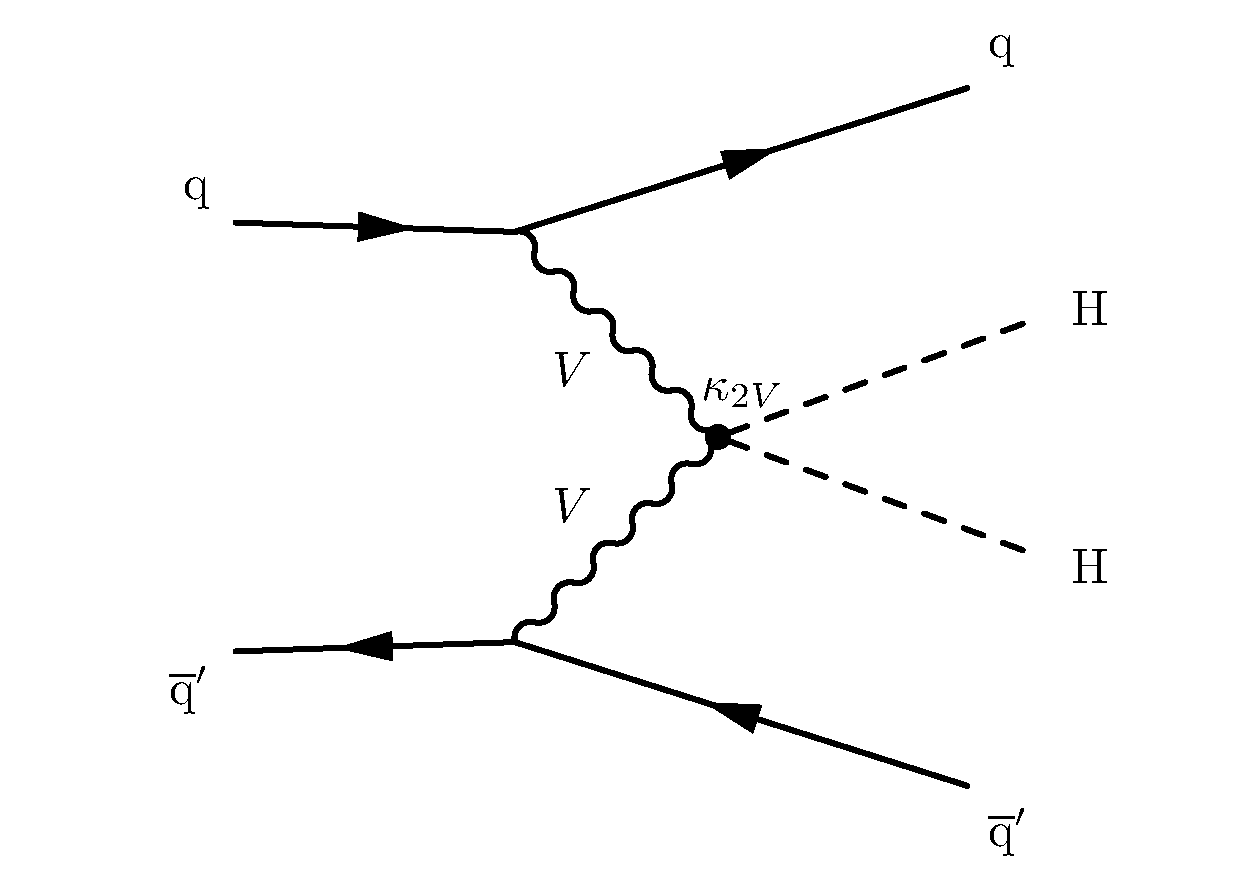
\includegraphics[width=0.32\textwidth]{figures/05-HH/production/diagrams/feynman_03.pdf}
    \caption{Leading-order diagrams for nonresonant \HH production via vector boson fusion.
    In this chapter, we refer to the left-most VBF diagram as the $(\HVV)^2$ and the right-most as the $\HHVV$ diagram.}
    \label{fig:05_feynmanvbf}
\end{figure}

The production cross section and kinematic properties of the \HH system are altered if values of the Higgs self-coupling, the top Yukawa coupling, and/or the quartic \HHVV coupling are modified due to beyond the SM (BSM) effects.
Notably, at the energy scale of the LHC, the leading contribution to the VBF production amplitude is the scattering of longitudinal vector bosons, which scales as $\sim m_{\PH\PH}^2 (\kapvv - \kappa_{\PV}^2)$~\cite{Bishara:2016kjn}, where, as above, \kapl, $\kapvv$, and $\kapv$ are defined to be multiplicative modifiers of the \HHH, \HHVV, and \HVV couplings from their SM values, respectively.

In the SM, with $\kapvv = \kapv = 1$, VBF production is suppressed since the left-most $(\HVV)^2$ and right-most \HHVV VBF diagrams in Figure~\ref{fig:05_feynmanvbf} cancel; however, BSM deviations to \HHVV can spoil the cancelation, significantly enhancing this mode.
This departure from the SM could be more visible at high energies, as illustrated in Figure~\ref{fig:05_intro_mhh}, which shows the increase and shift towards higher \mHH of the differential VBF \HH production cross section for enhanced and reduced \kapvv values.
Thus, measuring high-\mHH nonresonant VBF \HH production, with both Higgs bosons highly Lorentz-boosted, is a powerful probe of the \HHVV coupling.

\begin{figure}[ht]
    \centering
    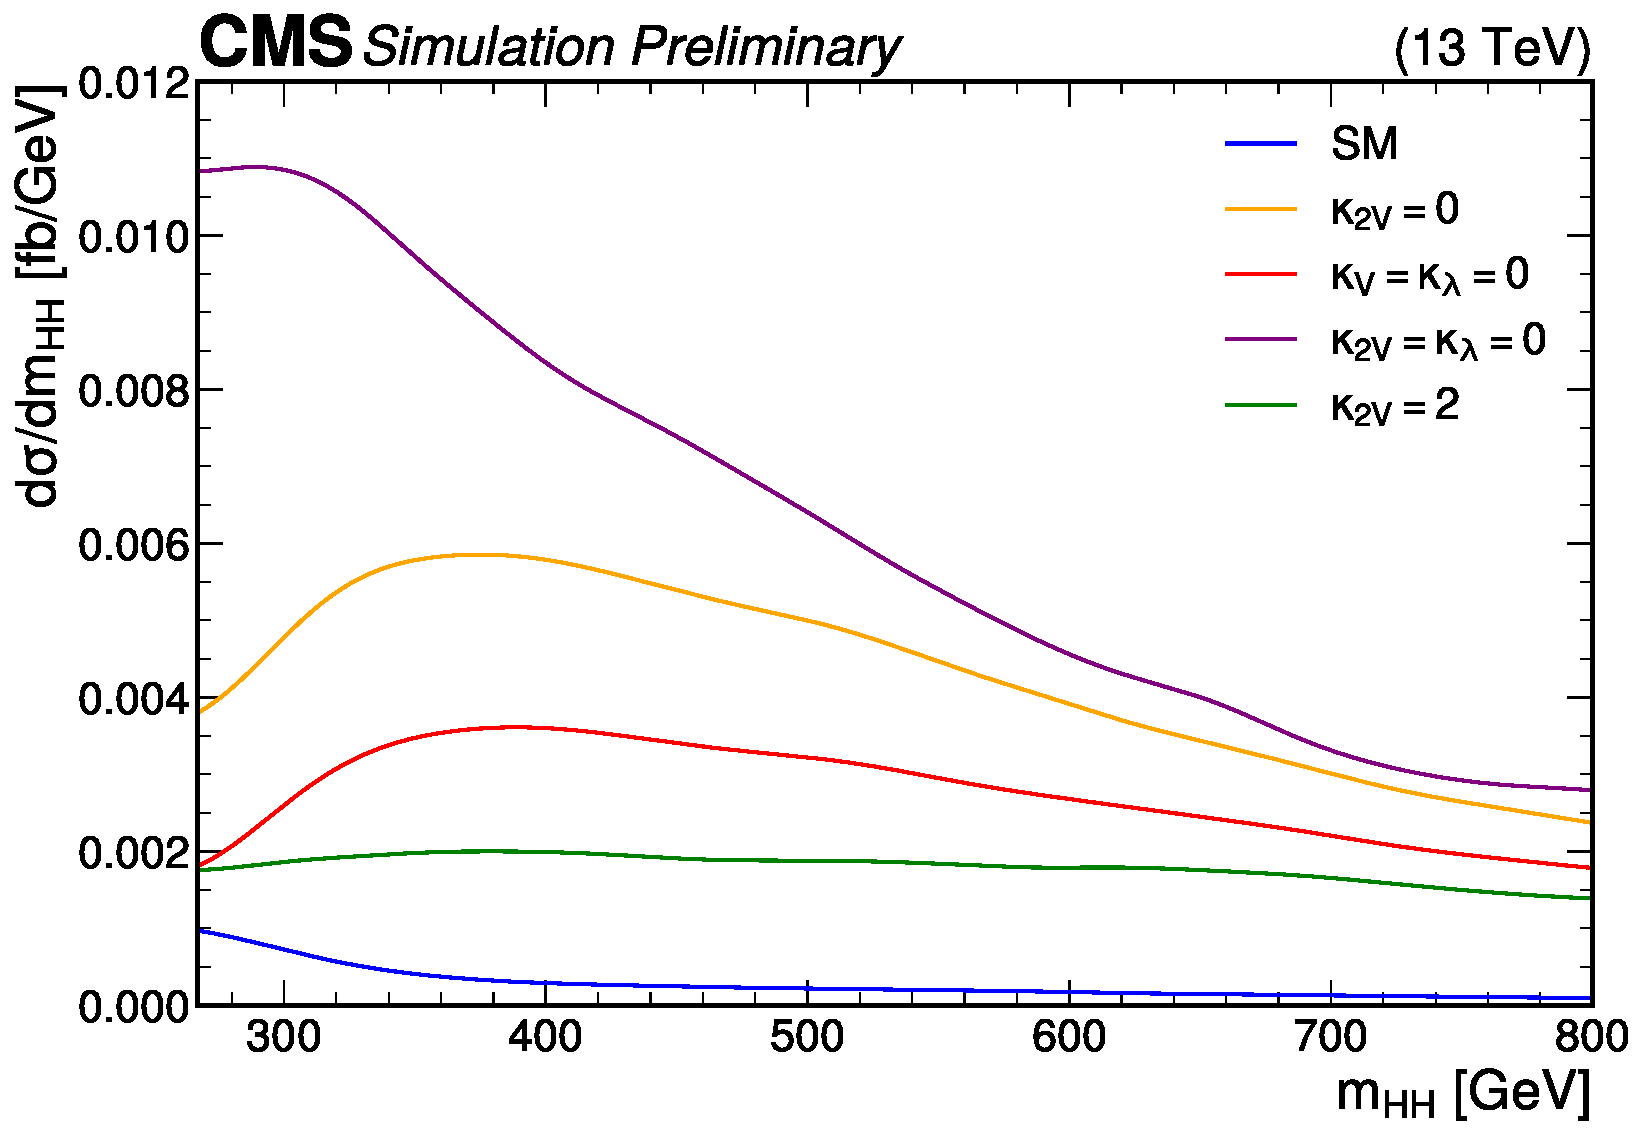
\includegraphics[width=0.7\textwidth]{figures/05-HH/production/diagrams_prelim.pdf}
    \caption{Differential cross section at $13\TeV$ center of mass for VBF \HH production as a function of the invariant mass of the \HH system (\mHH) for different diagrams and couplings.}
    \label{fig:05_intro_mhh}
\end{figure}

This is evidenced by the current \kapvv constraint in CMS being dominated by the search for boosted \HH in the \bbbb channel, with an observed (expected) 95\% confidence level (\CL) constraint of $[0.6, 1.4]$ ($[0.7, 1.4]$), excluding $\kapvv = 0$ for the first time~\cite{CMS:2022gjd}.
This is followed by CMS searches in the resolved \bbbb~\cite{CMS:2022cpr} and \bbtautau~\cite{CMS:2022hgz} channels, with constraints of $[-0.1, 2.2]$ ($[-0.4, 2.5]$) and $[-0.4, 2.6]$ ($[-0.6, 2.8]$), respectively.
Similarly, the strongest \kapvv constraint from the ATLAS experiment is from the boosted \bbbb search~\cite{ATLAS-CONF-2024-003}, with an observed (expected) 95\% \CL constraint of $[0.55, 1.49]$ ($[0.3, 1.7]$).

The success of searches in the boosted \bbbb channel motivates further exploration of high-\mHH \HH production.
This dissertation presents the first search in the all-hadronic \bbvv channel, where one Higgs boson decays to \bbbar while the other to \ww or \zz, where $\PW\to\qqbar$ and $\PZ\to\qqbar$.
The branching fractions for the \bbbar and all-hadronic \VV decays are $0.58$ and $0.11$ respectively, for a total branching fraction $\mathcal{B}(\HHbbVVq) = 2  \cdot0.58\cdot 0.11 = 0.13$, which is the second largest behind \bbbb.
The analysis primarily aims to constrain \kapvv and also sets an exclusion limit on the inclusive \HH production cross-section.
It is not expected to be sensitive to \kapl because of the focus on the high-\mHH regime.

Another benefit of the high-\mHH regime is the significantly reduced QCD multijet background, which otherwise makes such all-hadronic searches extremely challenging.
Because of the two Higgs bosons' high Lorentz-boosts, this regime also features the unique experimental signature of the \bbbar and \VVq decays each being reconstructed as single wide-radius jets.
Such merged \hbb jets have been identified to great effect in CMS using deep neural networks (DNNs)~\cite{CMS:2023tlv, CMS:2022gjd}, but attaining similar signal versus background discrimination for \hvv jets remains an open challenge.
To this end, we introduce a new attention-based DNN, referred to as the global particle transformer (GloParT) to not only enable this search but open new possibilities for searches in boosted-\VV channels as well (Chapter~\ref{sec:05_jet_tagging}).

\subsection{Experimental status of \HH measurements with CMS}
\label{sec:05_smhh_golden_channels}

\begin{figure}[ht]
    \centering
    % \captionsetup{justification=centering}
    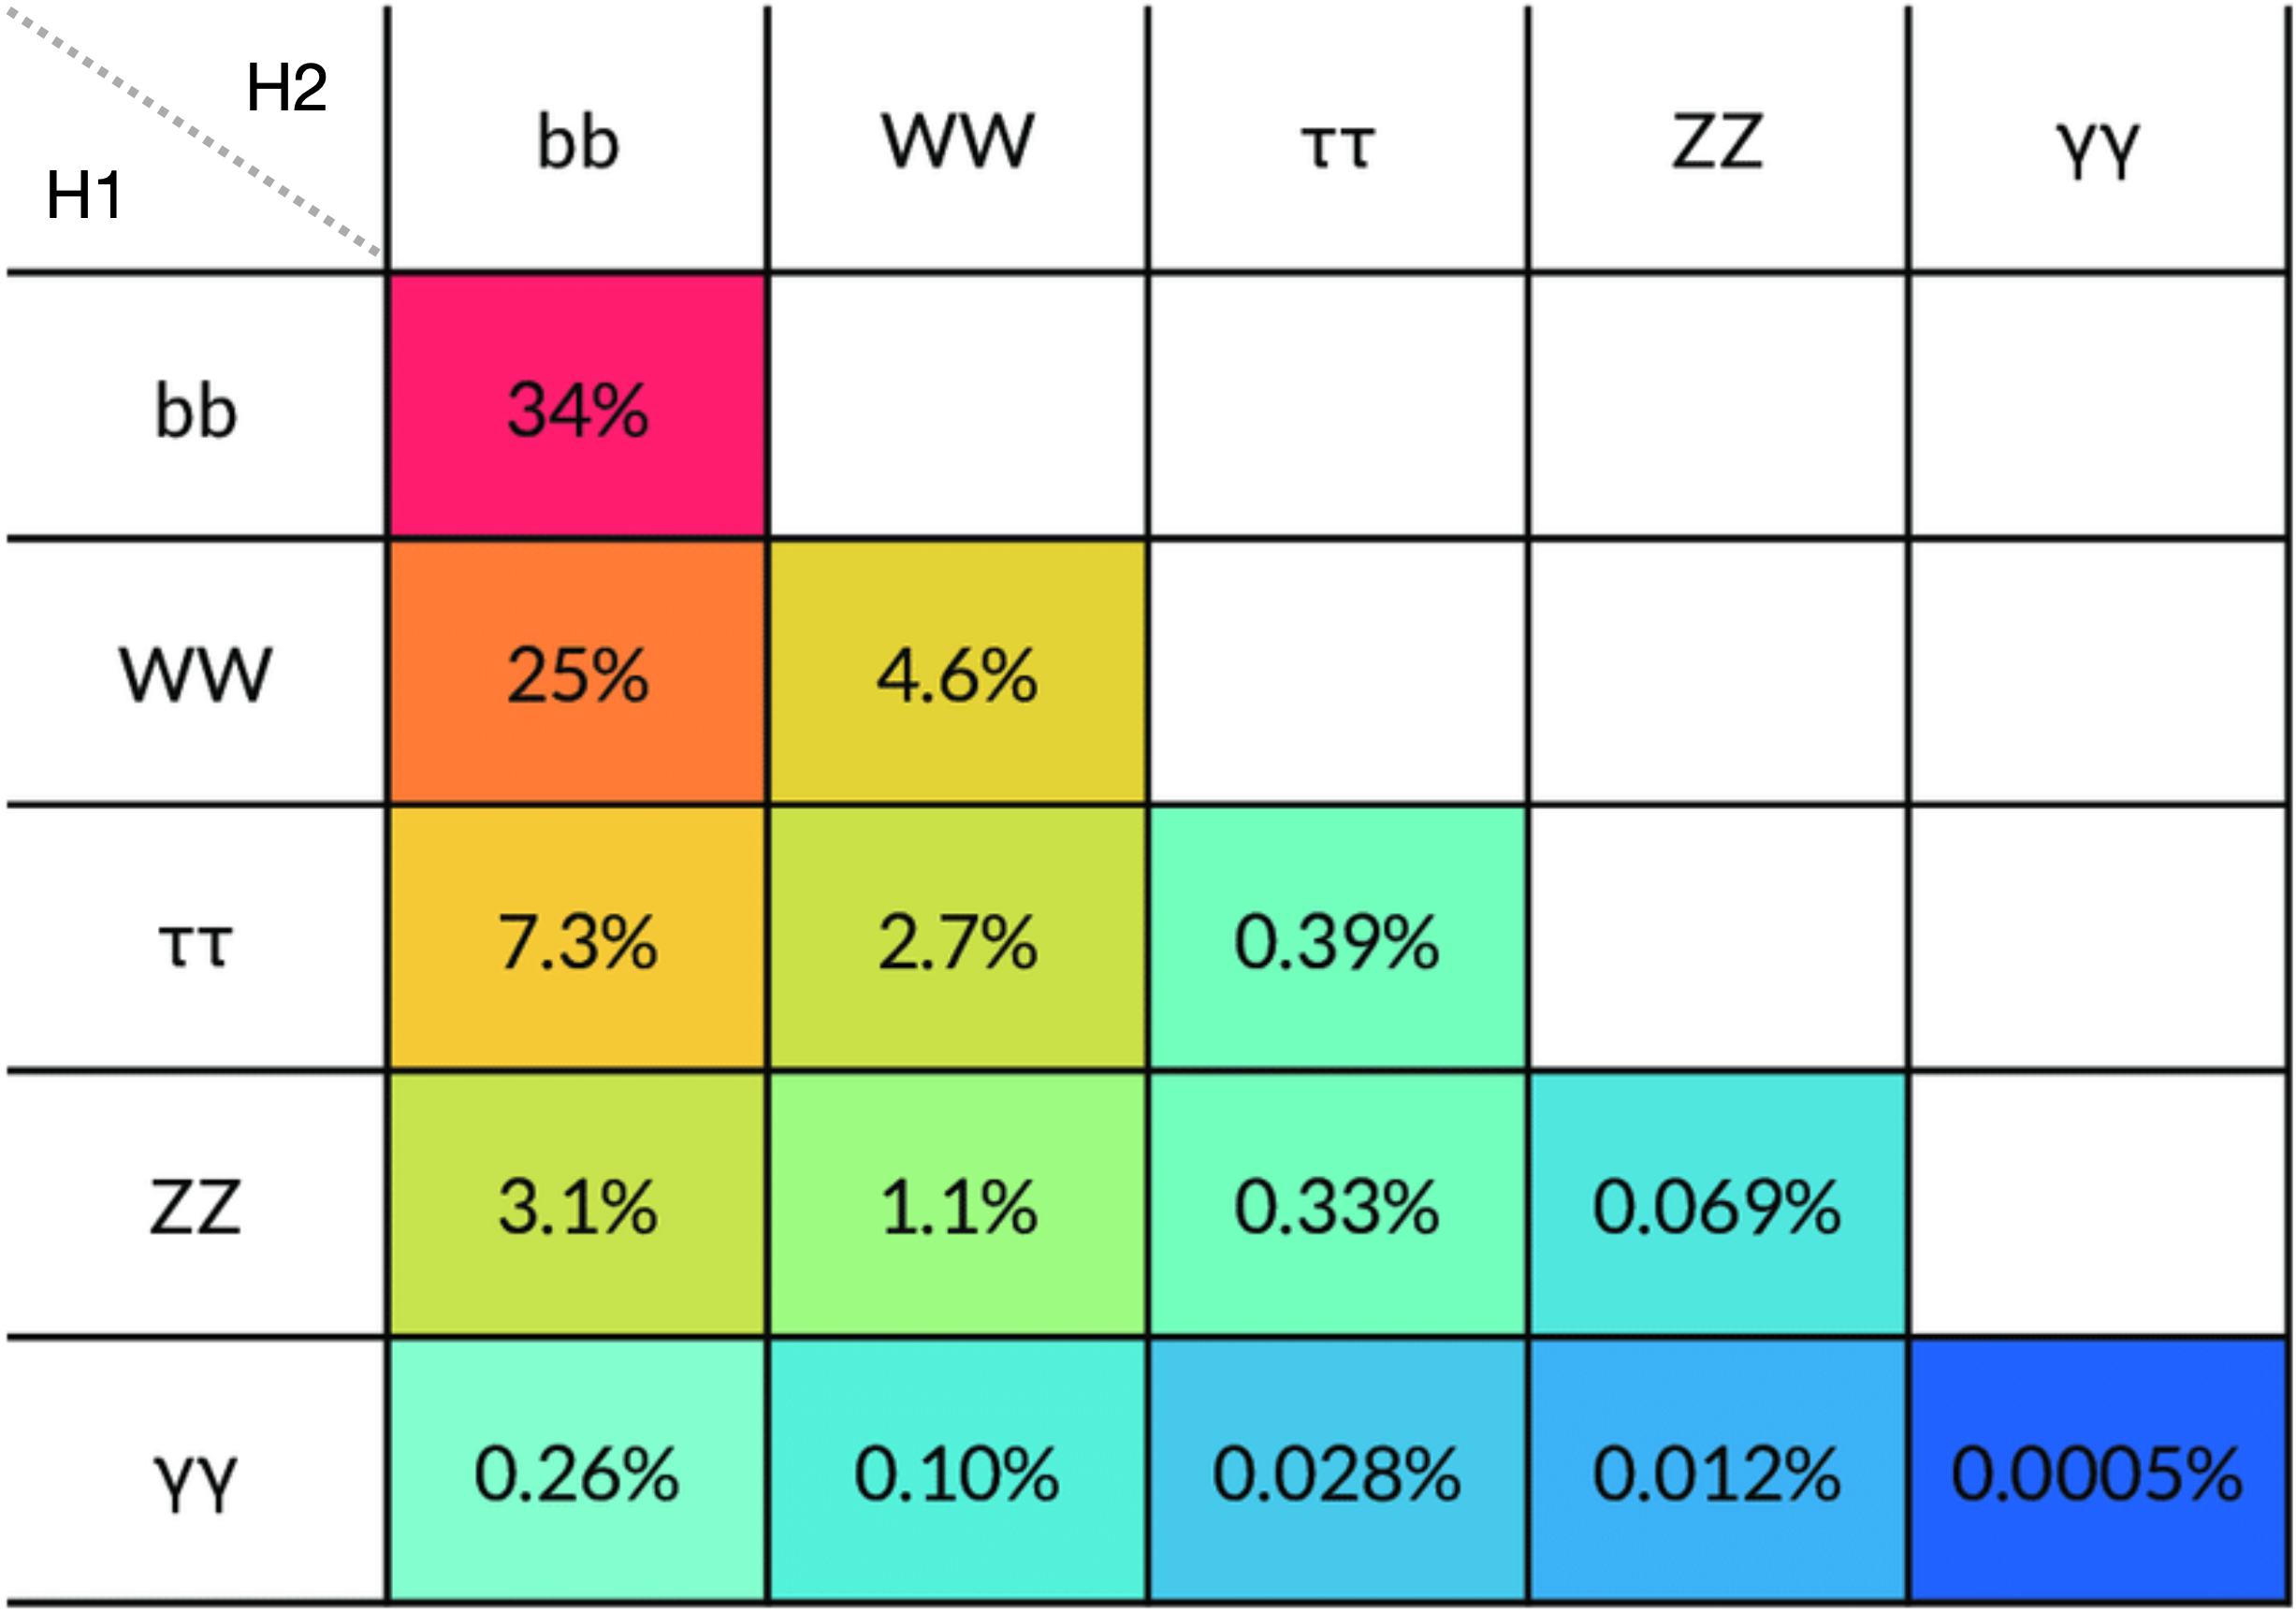
\includegraphics[width=0.6\textwidth]{figures/05-HH/CMS-results/HHBRs.png}
    \caption{\HH decays and their respective branching fractions (reproduced from Ref.~\cite{Veatch:2022uzz}).}
    \label{fig:05_hhbrs}
\end{figure}

The decays and branching fractions (BFs) of the Higgs boson pairs are shown in Figure~\ref{fig:05_hhbrs}.
Three of these final states have emerged as experimental ``golden channels'' --- the channels expected to yield the highest signal-to-background-events ratio for SM \HH production:
\begin{itemize}
    \item \bbbb:\quad This channel has the highest BF ($34\%$) and, despite the large QCD multijet background due to the all-hadronic final state, it benefits from unique signatures of heavy-flavor \Pb-jets, such as the presence of secondary vertices and displaced tracks due to the long lifetimes of \Pb-hadrons.
    Both the resolved~\cite{CMS:2022cpr} and boosted~\cite{CMS:2022gjd} Run 2 CMS analyses (Figure~\ref{fig:05_bbbb_run2}) have been highly effective, with the latter benefitting from the high BF of this decay mode, the exponential reduction of the QCD multijet background in the boosted regime, and significant recent advances in \bbbar-jet classification and reconstruction (as will be discussed in Chapter~\ref{sec:05_jet_tagging}).
    \item \bbtautau:\quad This has an intermediate BF of $7\%$ but relatively lower background of primarily Drell-Yan ($\PZ/\PGg^*$), top quark pair production (\ttbar), and QCD multijet events (Figure~\ref{fig:05_bbtautau}, reproduced from Ref.~\cite{CMS:2022hgz}).
    It benefits from similar deep learning techniques for \Pb-jet tagging, and targets all-hadronic ($\PGt_h\PGt_h$) and semi-leptonic ($\PGt_h\PGt_e$ or $\PGt_h\PGt_\mu$) \PGt-lepton decays using a variety of traditional and ML techniques.
    \item \bbgg:\quad Despite the small BF ($0.3\%$) of this channel, the $\PH\to\PGg\PGg$ decay provides a clean experimental signature with a sharply peaking resonance over a small background of QCD multijet + $\PGg$ events (Figure~\ref{fig:05_bbgg}, from Ref.~\cite{CMS:2020tkr}).
\end{itemize}

More recently, the \bbww channel has been explored in the douple-lepton ($\Pl\Pl\nu\nu$) and single-lepton ($\Pl\nu\Pq\Pq$) \ww final states~\cite{CMS:2024rgy}, which have a large combined BF of $13.4\%$.
The former features a clean experimental signature of two opposite-sign leptons but a small BF of $2.6\%$, while the latter has the higher BF of 10.8\% but larger top quark background as well (Figure~\ref{fig:05_bbww}).
Because of this, the two channels have similar sensitivities to the \HH cross section.

\begin{figure}[htb!]
    \centering
    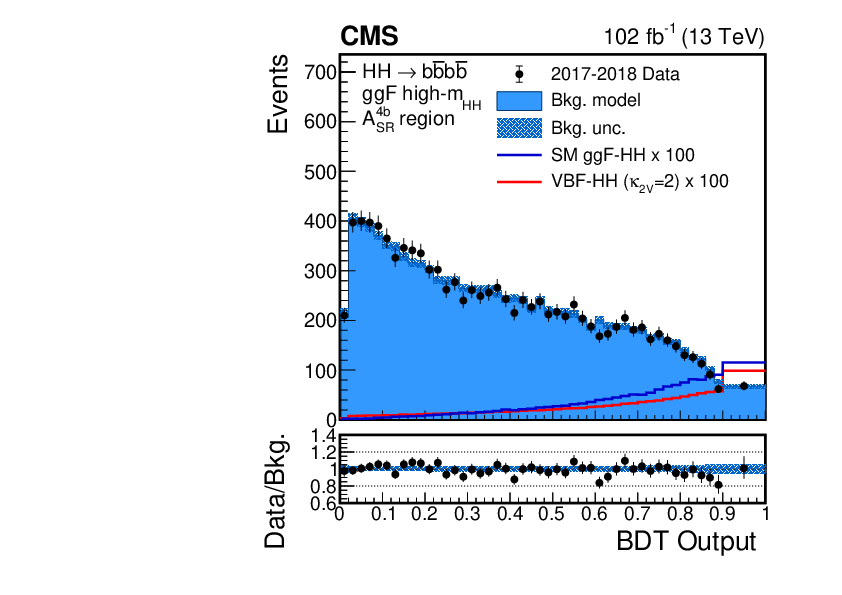
\includegraphics[trim=260pt 20pt 40pt 20pt, clip, width=0.31\textwidth]{figures/05-HH/CMS-results/4b/Figure_001-e.png}
    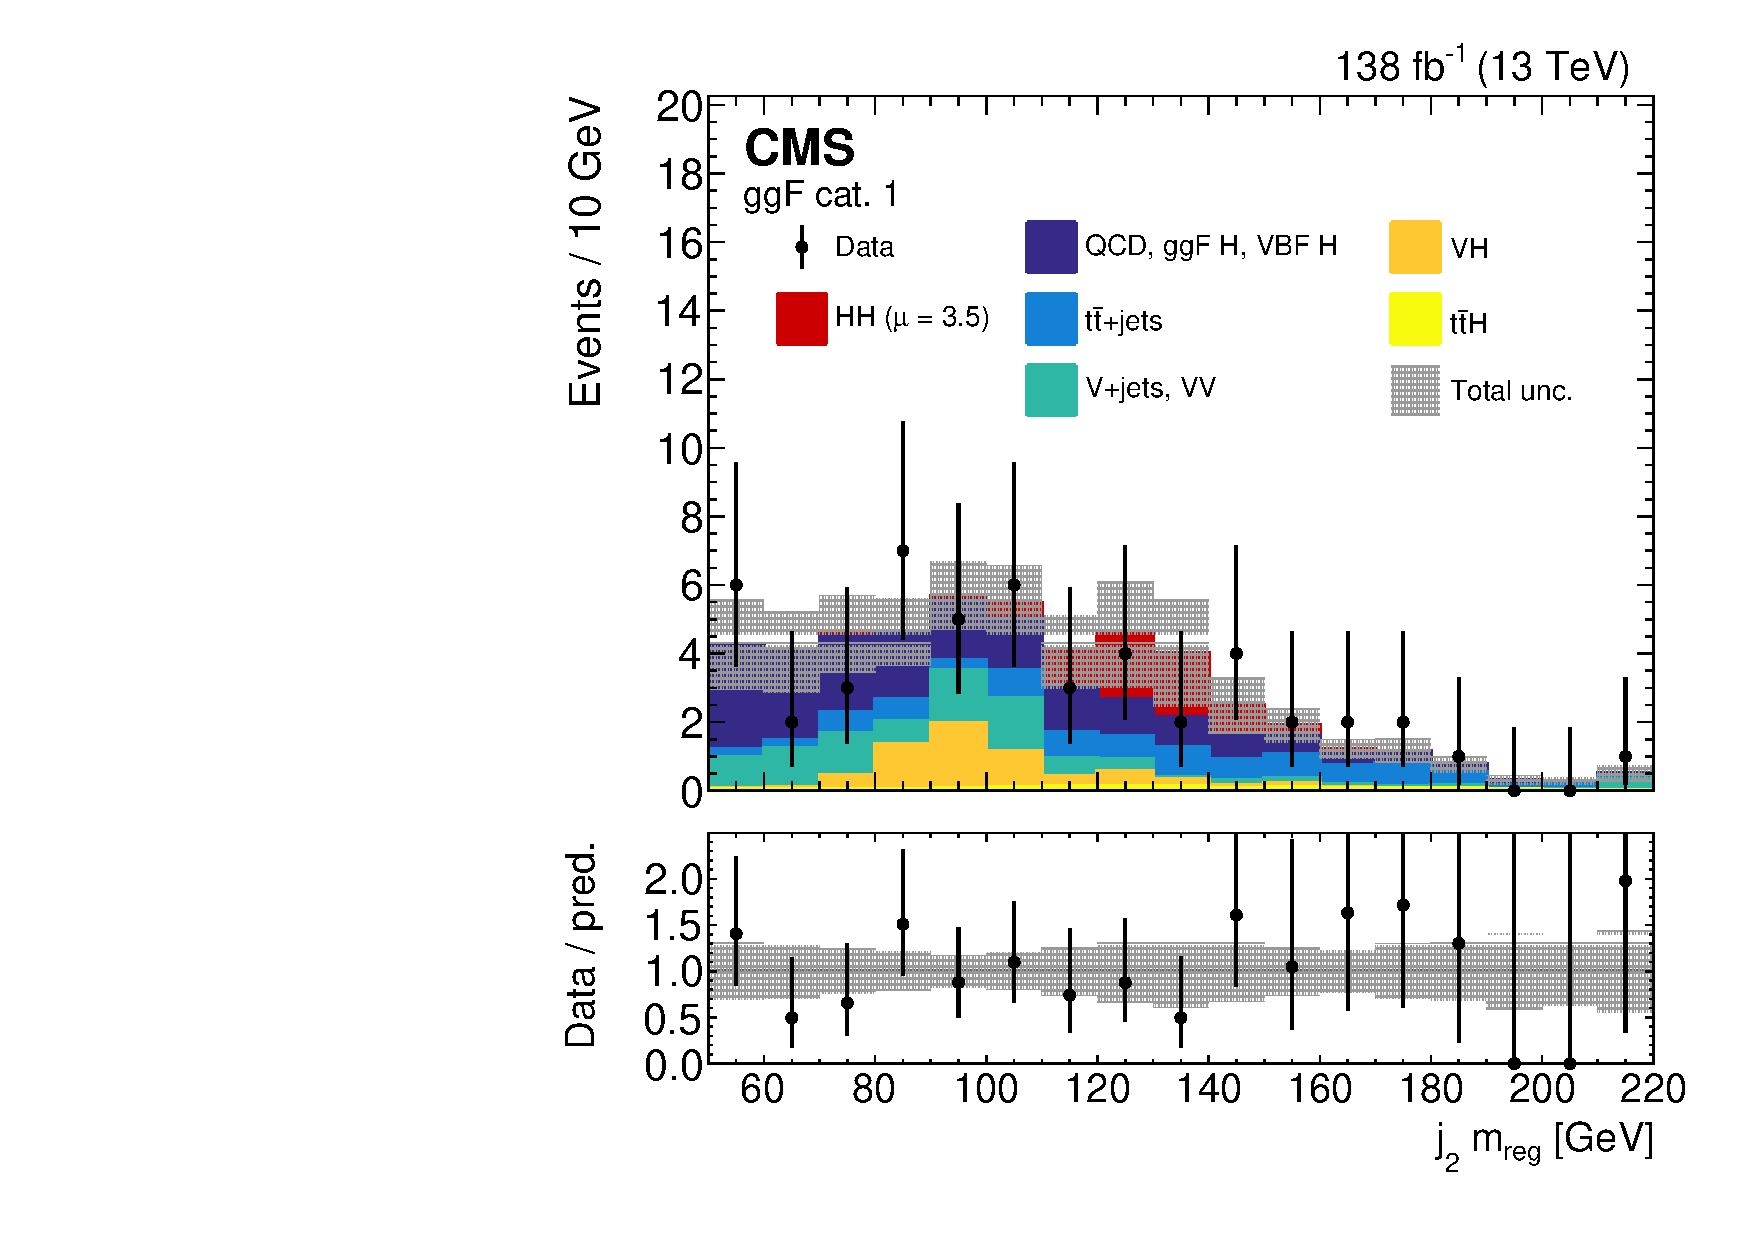
\includegraphics[width=0.33\textwidth]{figures/05-HH/CMS-results/4b/CMS-B2G-22-003_Figure_001.pdf}
    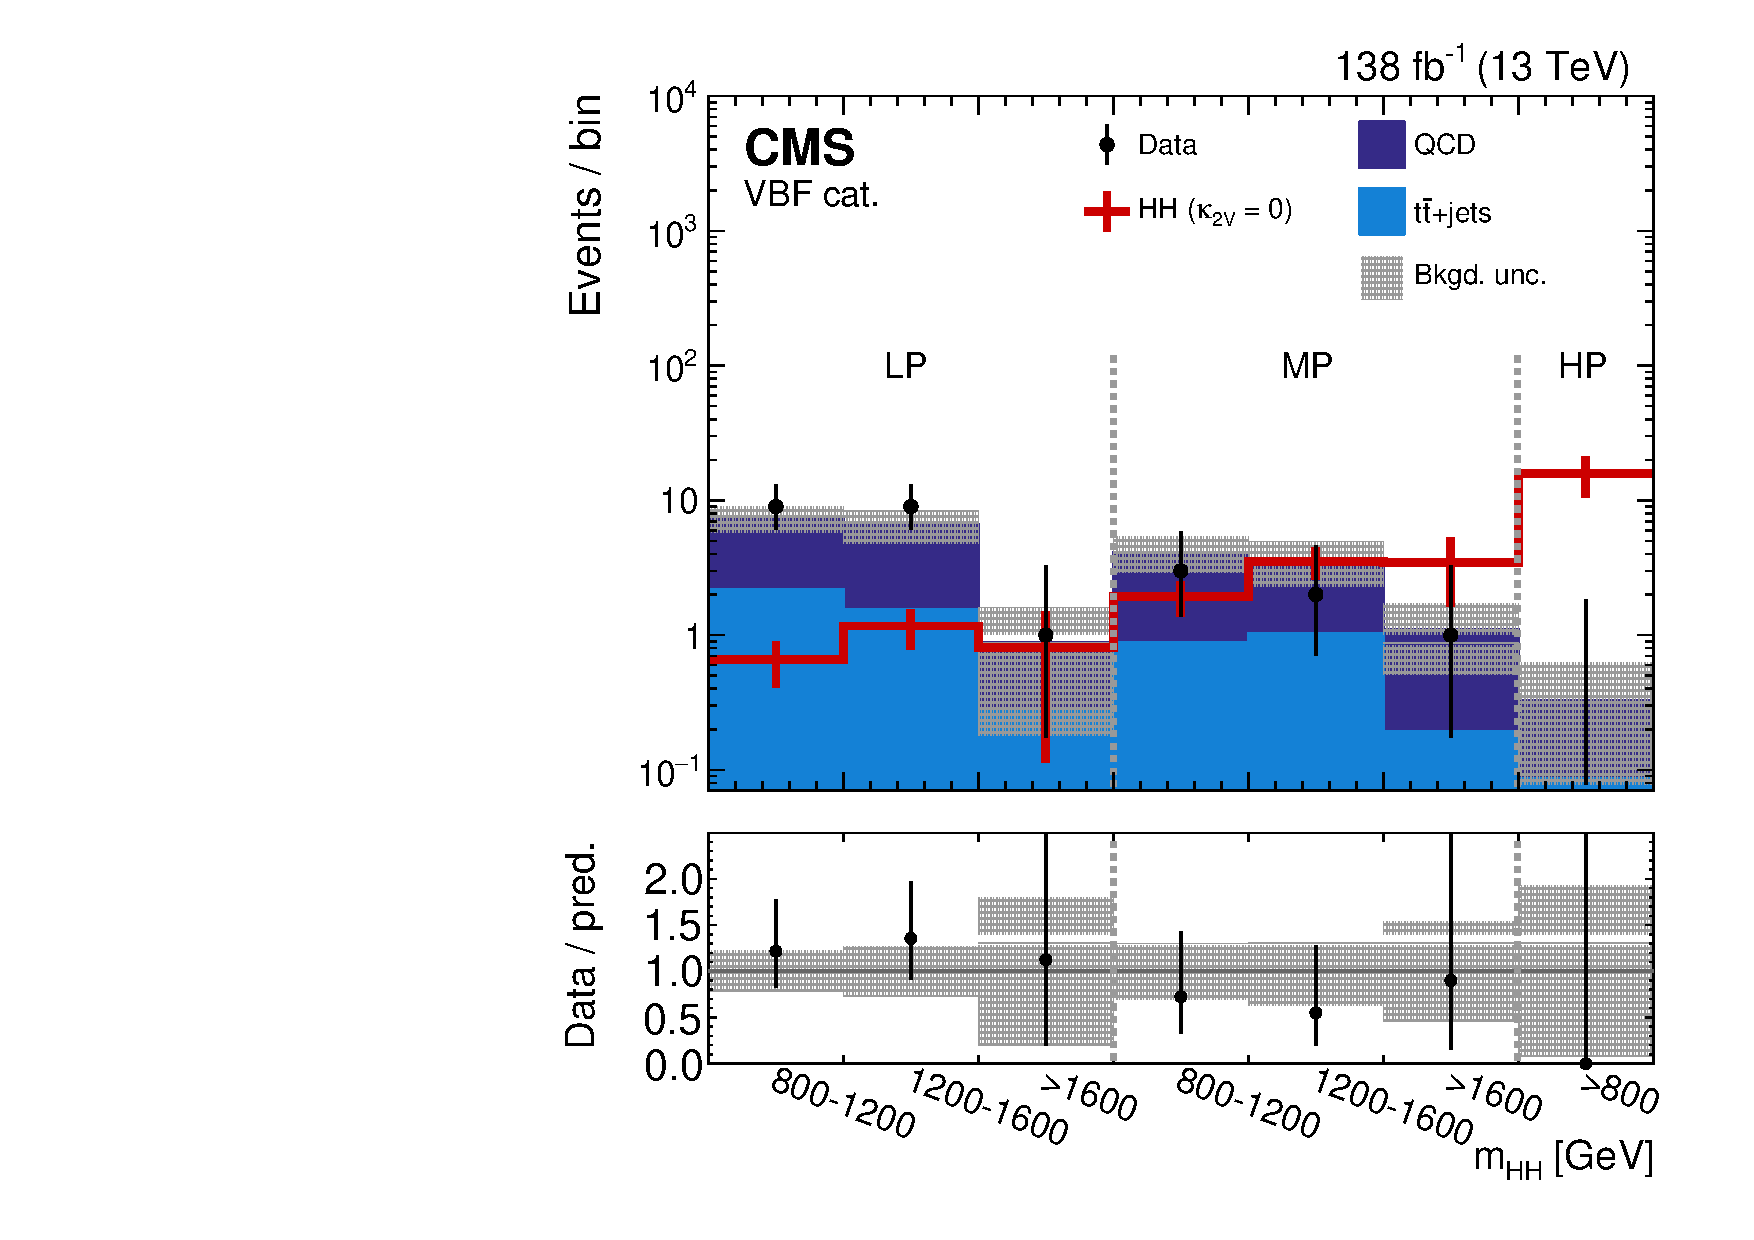
\includegraphics[width=0.33\textwidth]{figures/05-HH/CMS-results/4b/CMS-B2G-22-003_Figure_002.pdf}
    \caption[Distribution of events in the high-\mHH ggF category of the Run 2 CMS $\HH\to\bbbb$ resolved analysis~\cite{CMS:2022cpr}.]{Distribution of events in the high-\mHH ggF category of the Run 2 CMS $\HH\to\bbbb$ resolved analysis~\cite{CMS:2022cpr} as a function of the BDT discriminant (left), and of the Run 2 boosted analysis'~\cite{CMS:2022gjd} most sensitive ggF category, as a function of the second-highest tagged \bbbar-jet's mass (middle), and VBF categories, as a function of \mHH (right).}
    \label{fig:05_bbbb_run2}
\end{figure}

\begin{figure}[htb!]
    \centering
    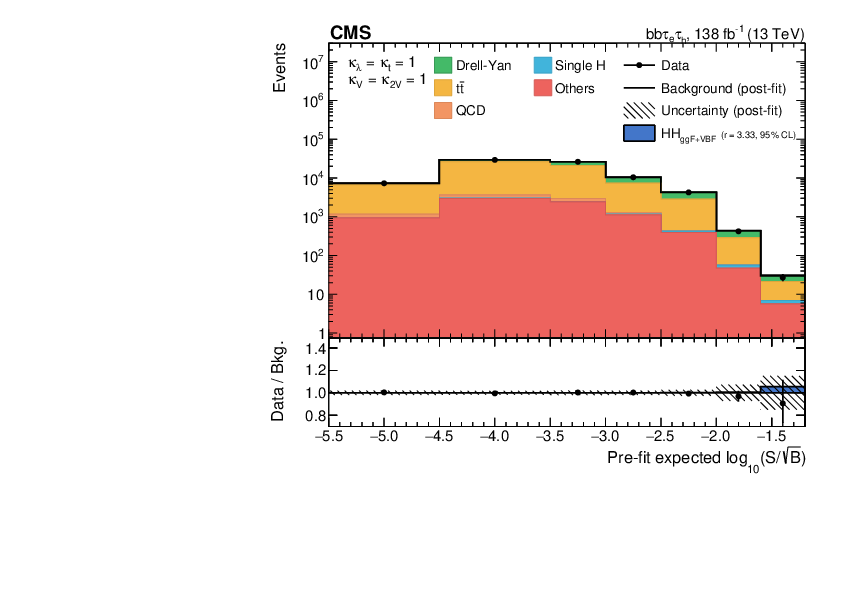
\includegraphics[trim=270pt 120pt 30pt 20pt, clip, width=0.32\textwidth]{figures/05-HH/CMS-results/bbtautau/Figure_005-a.png}
    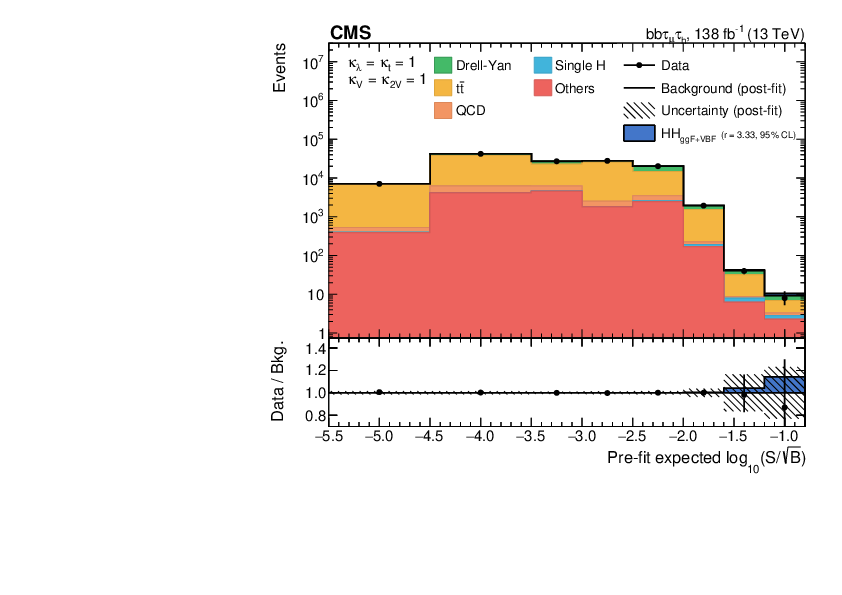
\includegraphics[trim=270pt 120pt 30pt 20pt, clip, width=0.32\textwidth]{figures/05-HH/CMS-results/bbtautau/Figure_005-b.png}
    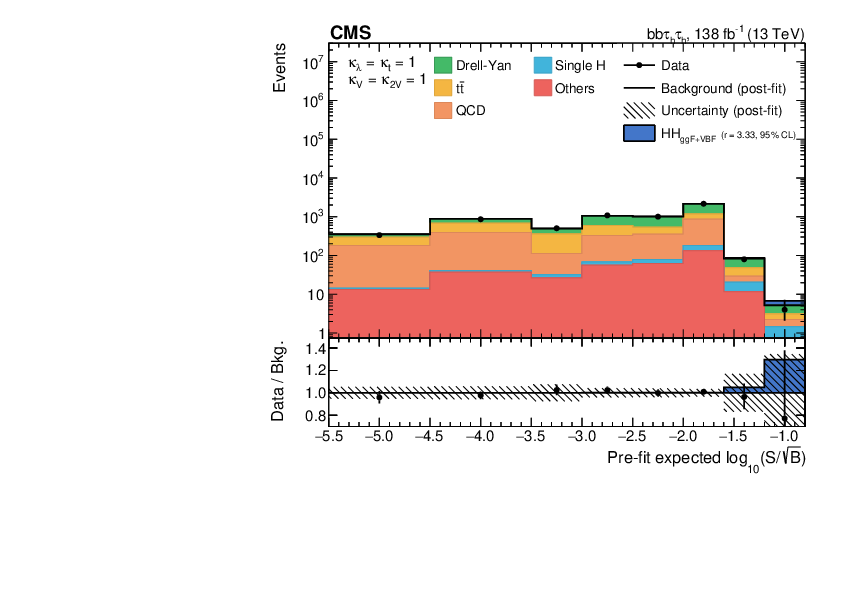
\includegraphics[trim=270pt 120pt 30pt 20pt, clip, width=0.32\textwidth]{figures/05-HH/CMS-results/bbtautau/Figure_005-c.png}
    \caption{Combination of bins of all postfit distributions of the Run 2 CMS $\HH\to\bbtautau$ analysis~\cite{CMS:2022hgz}, ordered according to the expected signal-to-square-root-background ratio, separately for the $\PGt_h\PGt_e$ (left), the $\PGt_h\PGt_\mu$ (center), and $\PGt_h\PGt_h$ (right) channels.}
    \label{fig:05_bbtautau}
\end{figure}

\begin{figure}[htb!]
    \centering
    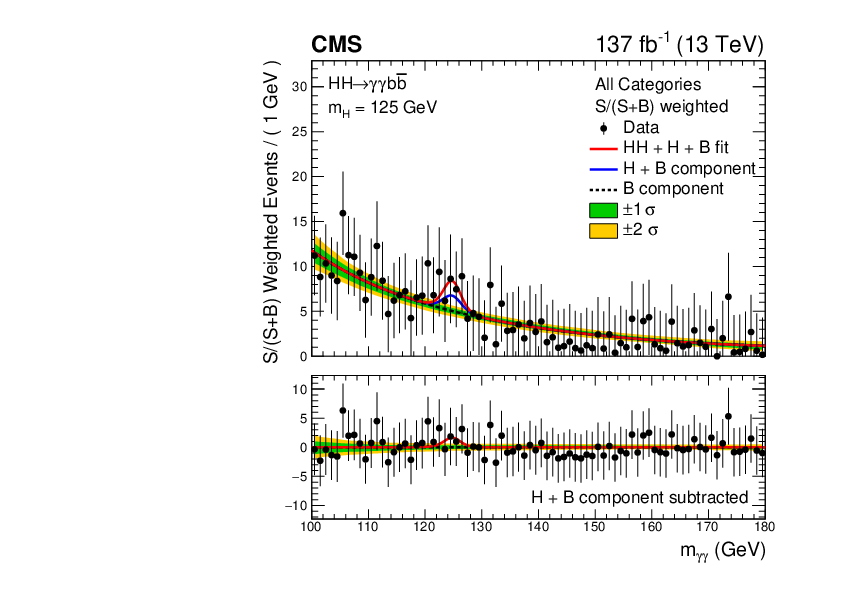
\includegraphics[trim=250pt 25pt 0 20pt, clip, width=0.5\textwidth]{figures/05-HH/CMS-results/bbgg.png}
    \caption[Invariant two-photon mass distribution of the Run 2 CMS $\HH\to\bbgg$ analysis~\cite{CMS:2020tkr}.]{Invariant two-photon mass distribution of the Run 2 CMS $\HH\to\bbgg$ analysis~\cite{CMS:2020tkr}, combined for all signal categories, weighted by S/(S+B), where S (B) is the number of signal (background) events extracted from the signal-plus-background fit.}
    \label{fig:05_bbgg}
\end{figure}

\begin{figure}[htb!]
    \centering
    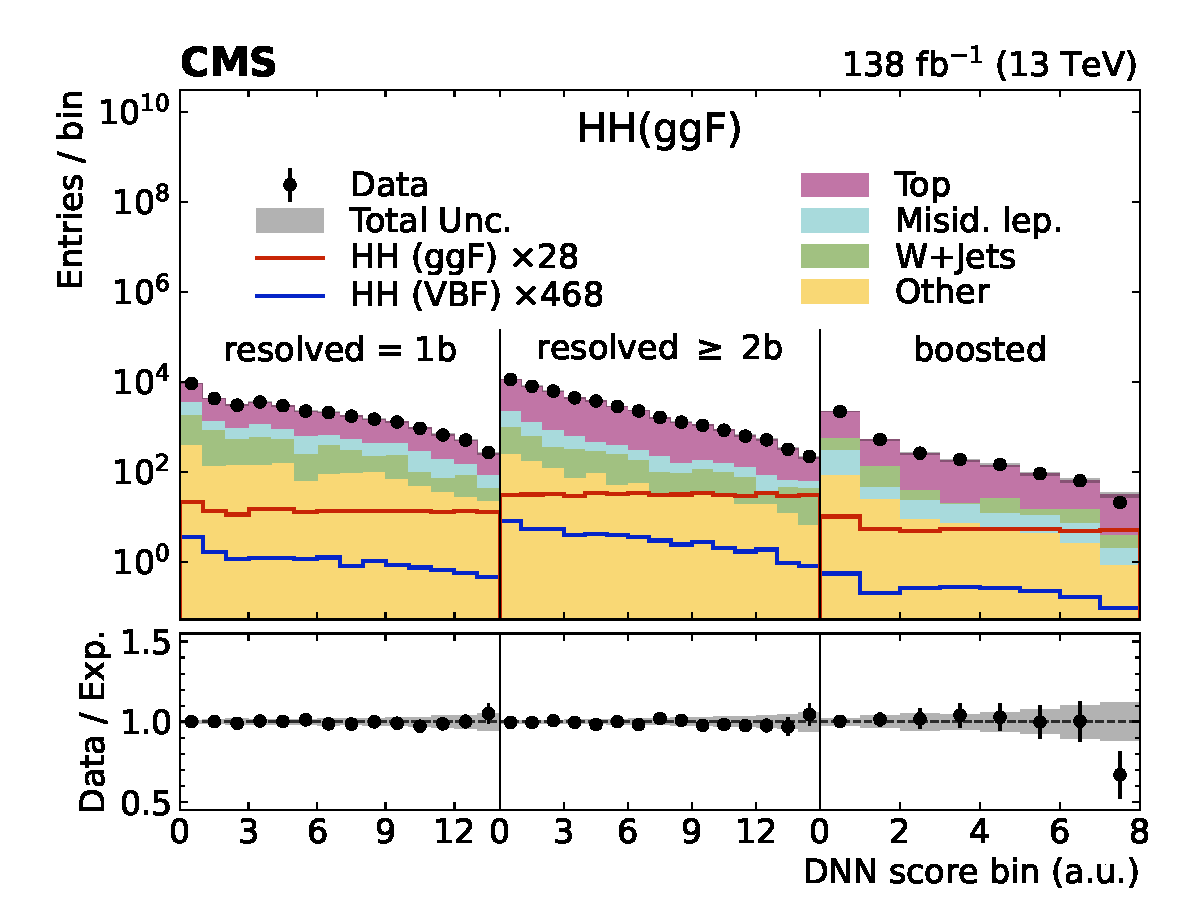
\includegraphics[width=0.49\textwidth]{figures/05-HH/CMS-results/bbww/CMS-HIG-21-005_Figure_005-a.pdf}
    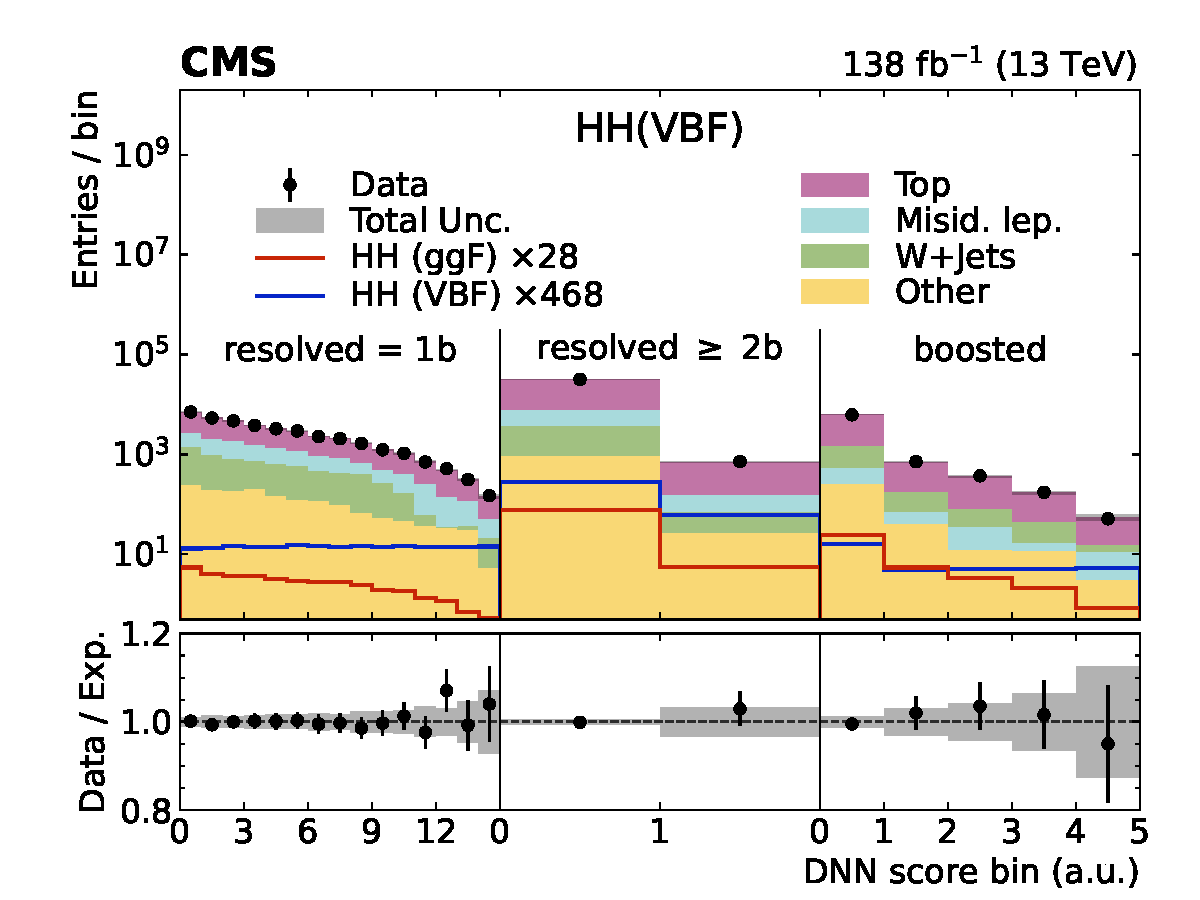
\includegraphics[width=0.49\textwidth]{figures/05-HH/CMS-results/bbww/CMS-HIG-21-005_Figure_005-b.pdf}
    \caption[Distribution of events in the resolved $1\Pb$, resolved $\geq2\Pb$, and boosted signal categories of the Run 2 CMS semi-leptonic $\HH\to\bbww$ analysis~\cite{CMS:2024rgy}.]{Distribution of events in the resolved $1\Pb$, resolved $\geq2\Pb$, and boosted signal categories of the Run 2 CMS semi-leptonic $\HH\to\bbww$ analysis~\cite{CMS:2024rgy} as a function of their DNN discriminant in the single-lepton (left) and double-lepton (right) final states.}
    \label{fig:05_bbww}
\end{figure}

The limits set on the \HH cross section by each channel, and their combinations, are shown in Figure~\ref{fig:05_hh_comb_xsec}, and as a function of \kapl and \kapvv in Figure~\ref{fig:05_hh_comb_kappa}.
The three ``golden channels'' each offer roughly similar sensitivities to the cross section and \kapl limits; however, the constraint on \kapvv is dominated by the boosted \bbbb channel, because of the enhancement of boosted \HH production at BSM \kapvv deviations, as discussed in Section~\ref{sec:05_smhh}.
Its observed (expected) $95\%$ confidence level (\CL) constraint is $[0.6, 1.4]$ ($[0.7, 1.4]$).
This is followed by the resolved \bbbb~\cite{CMS:2022cpr} and \bbtautau~\cite{CMS:2022hgz} channels, with constraints of $[-0.1, 2.2]$ ($[-0.4, 2.5]$) and $[-0.4, 2.6]$ ($[-0.6, 2.8]$), respectively.
Similarly, the strongest \kapvv constraint from the ATLAS experiment is from the recent boosted \bbbb search~\cite{ATLAS-CONF-2024-003}, with an observed (expected) $95\%$ \CL constraint of $[0.55, 1.49]$ ($[0.3, 1.7]$).

\begin{figure}[htb!]
    \centering
    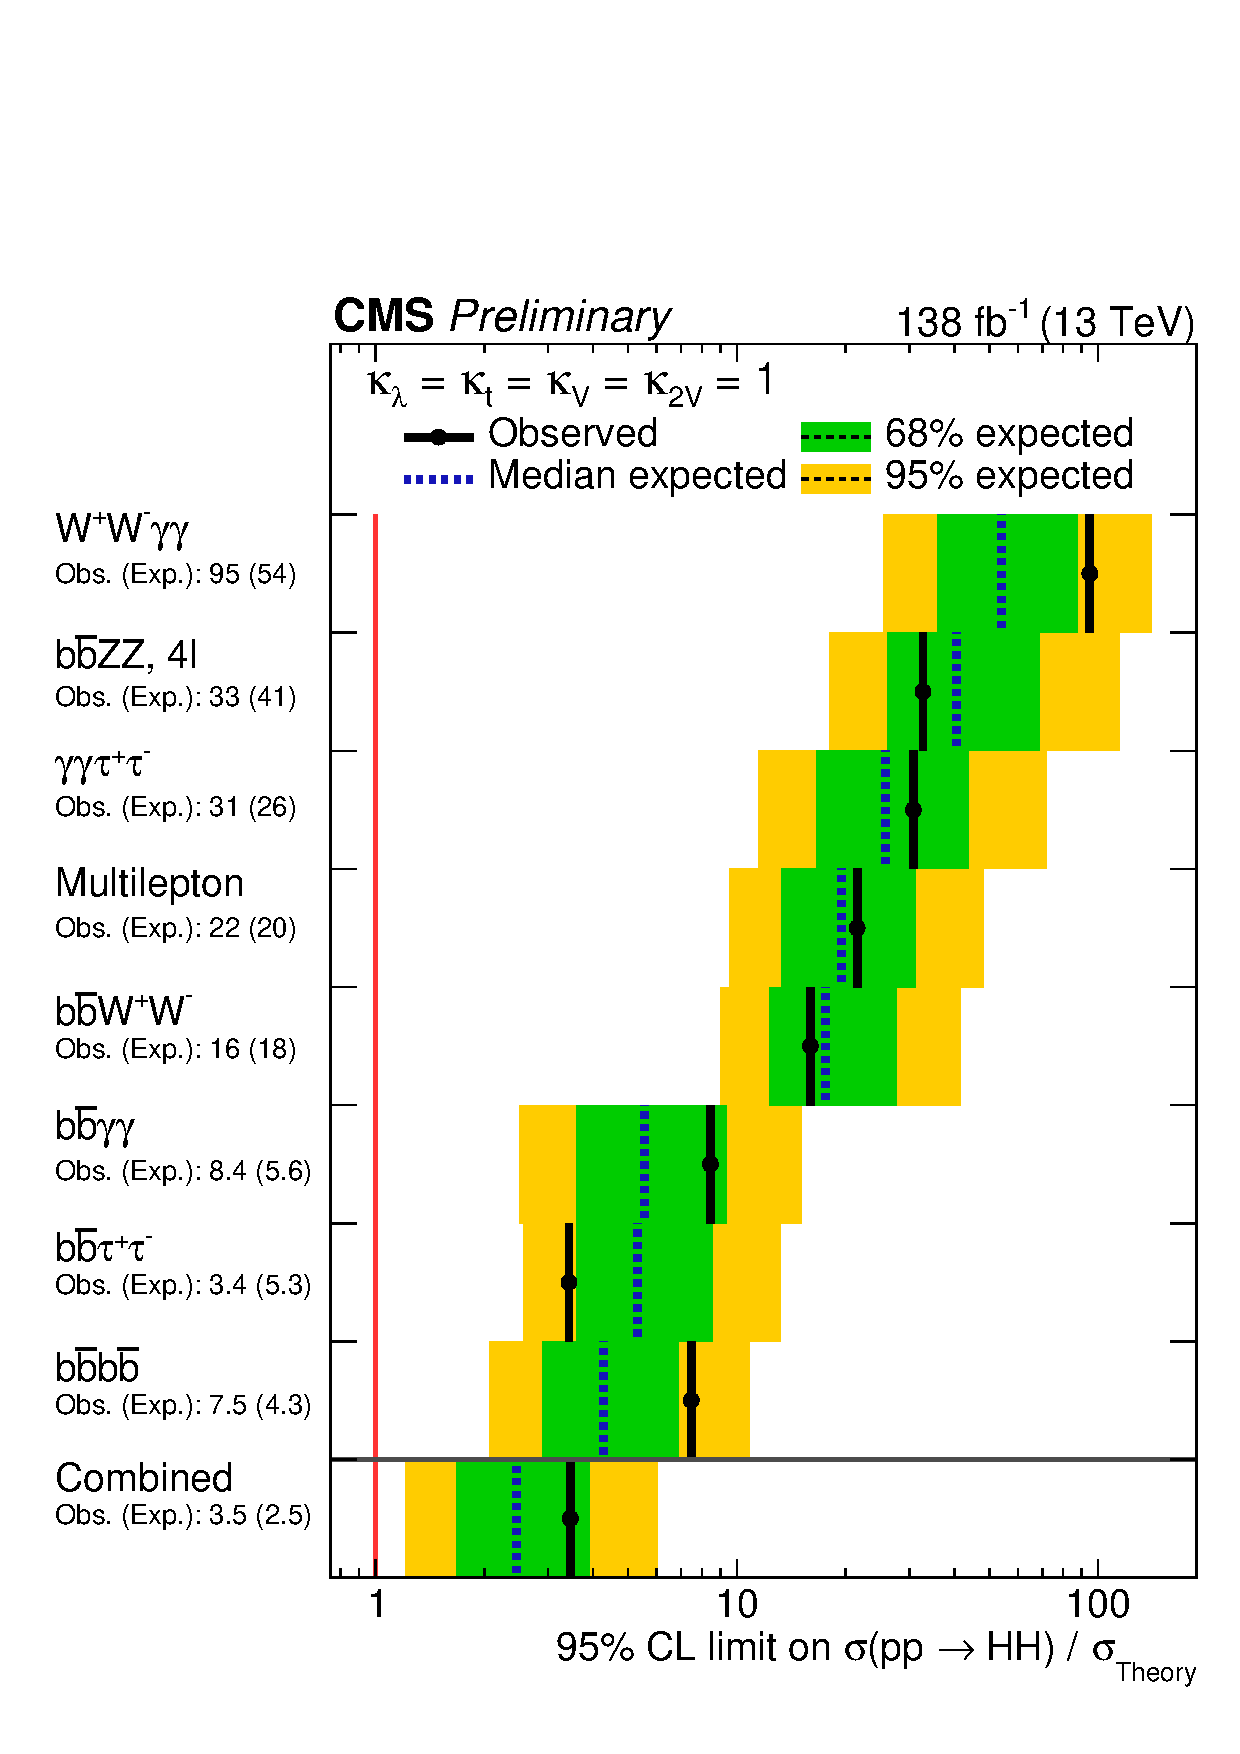
\includegraphics[width=0.8\textwidth]{figures/05-HH/CMS-results/HHcomb_xsec.pdf}
    \caption[The expected and observed limits on the ratio of experimentally estimated production cross section and the expectation from the SM in searches using different final states and their combination, reproduced from Ref.~\cite{CMS-PAS-HIG-20-011}.]{The expected and observed limits on the ratio of experimentally estimated production cross section and the expectation from the SM in searches using different final states and their combination, reproduced from Ref.~\cite{CMS-PAS-HIG-20-011}.
    The search modes are ordered, from upper to lower, by their expected sensitivities from the least to the most sensitive. The overall combination of all searches is shown by the lowest entry.}
    \label{fig:05_hh_comb_xsec}
\end{figure}

\begin{figure}[htb!]
    \centering
    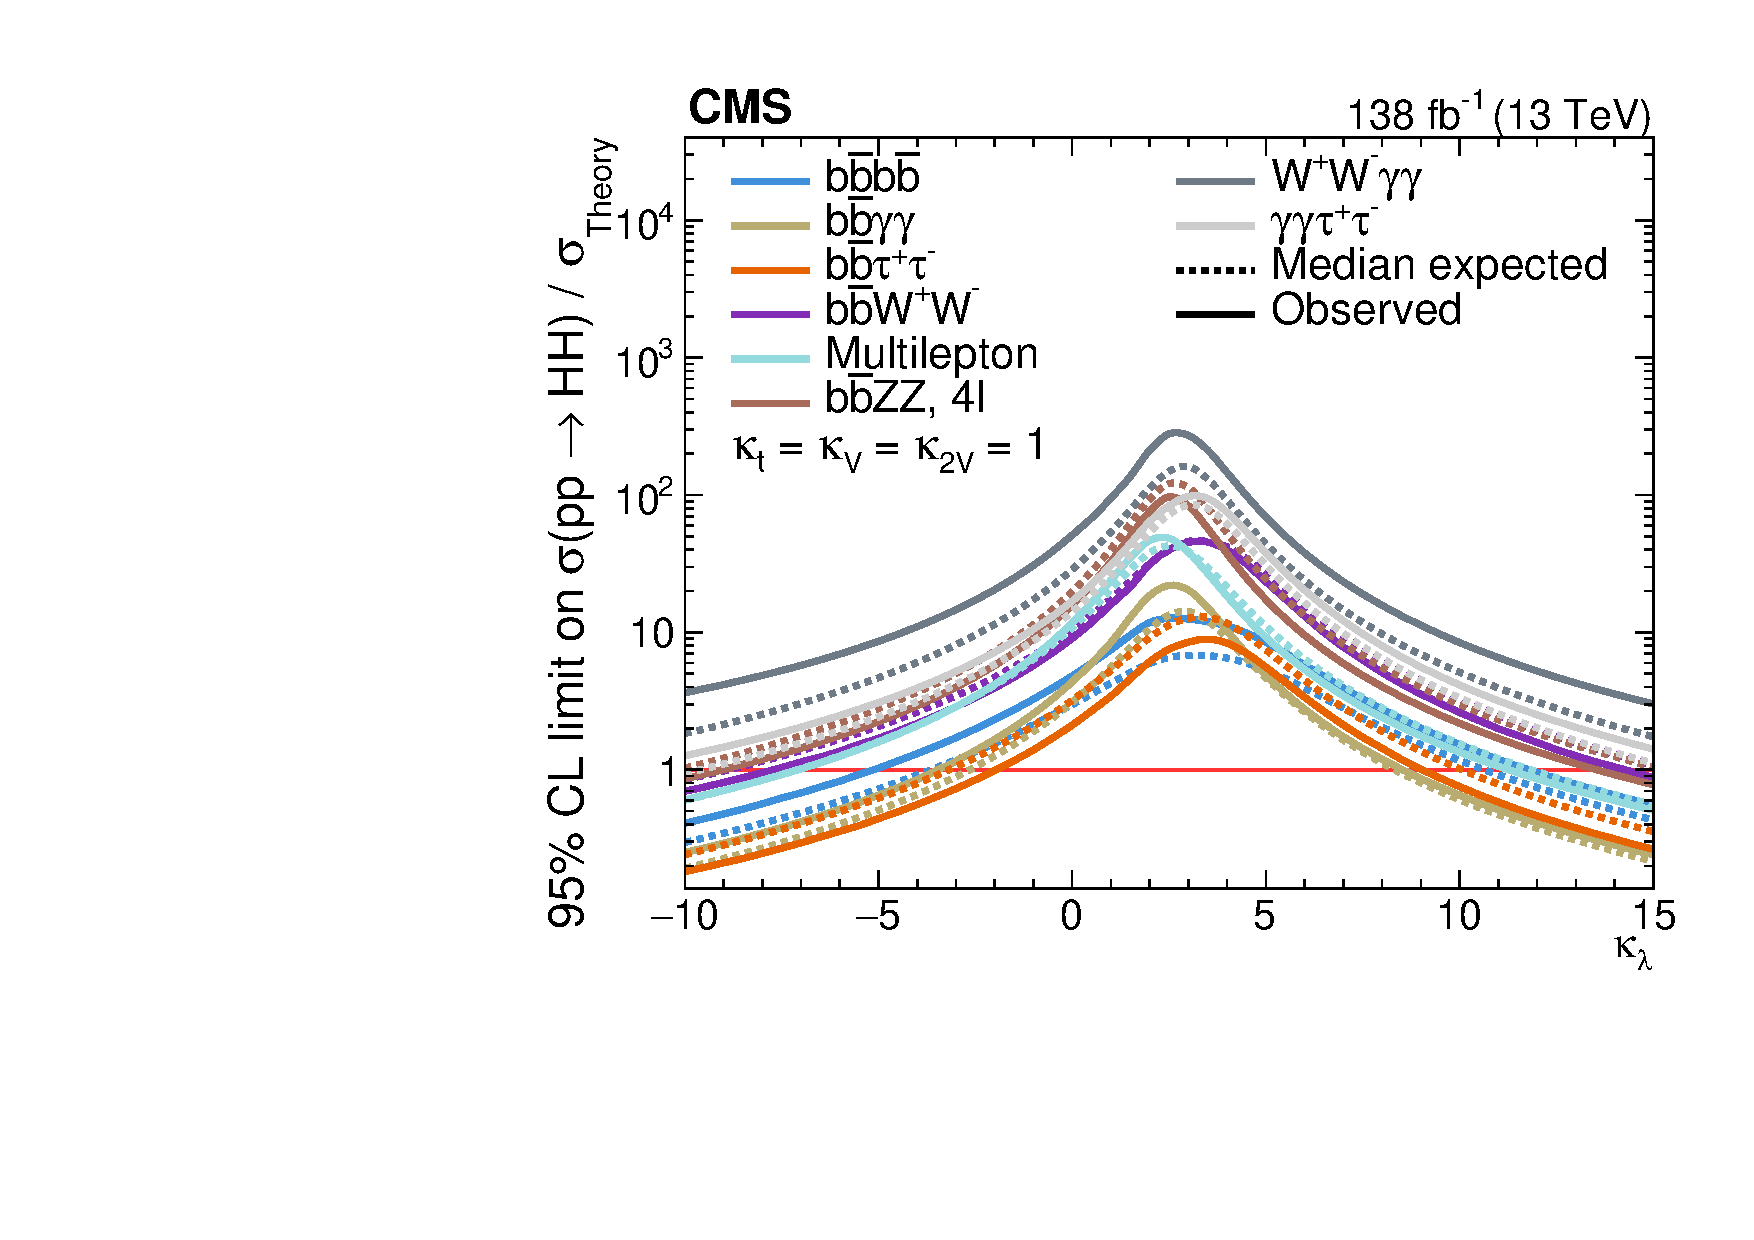
\includegraphics[width=0.49\textwidth]{figures/05-HH/CMS-results/kl_limits_channels_r_paper.pdf}
    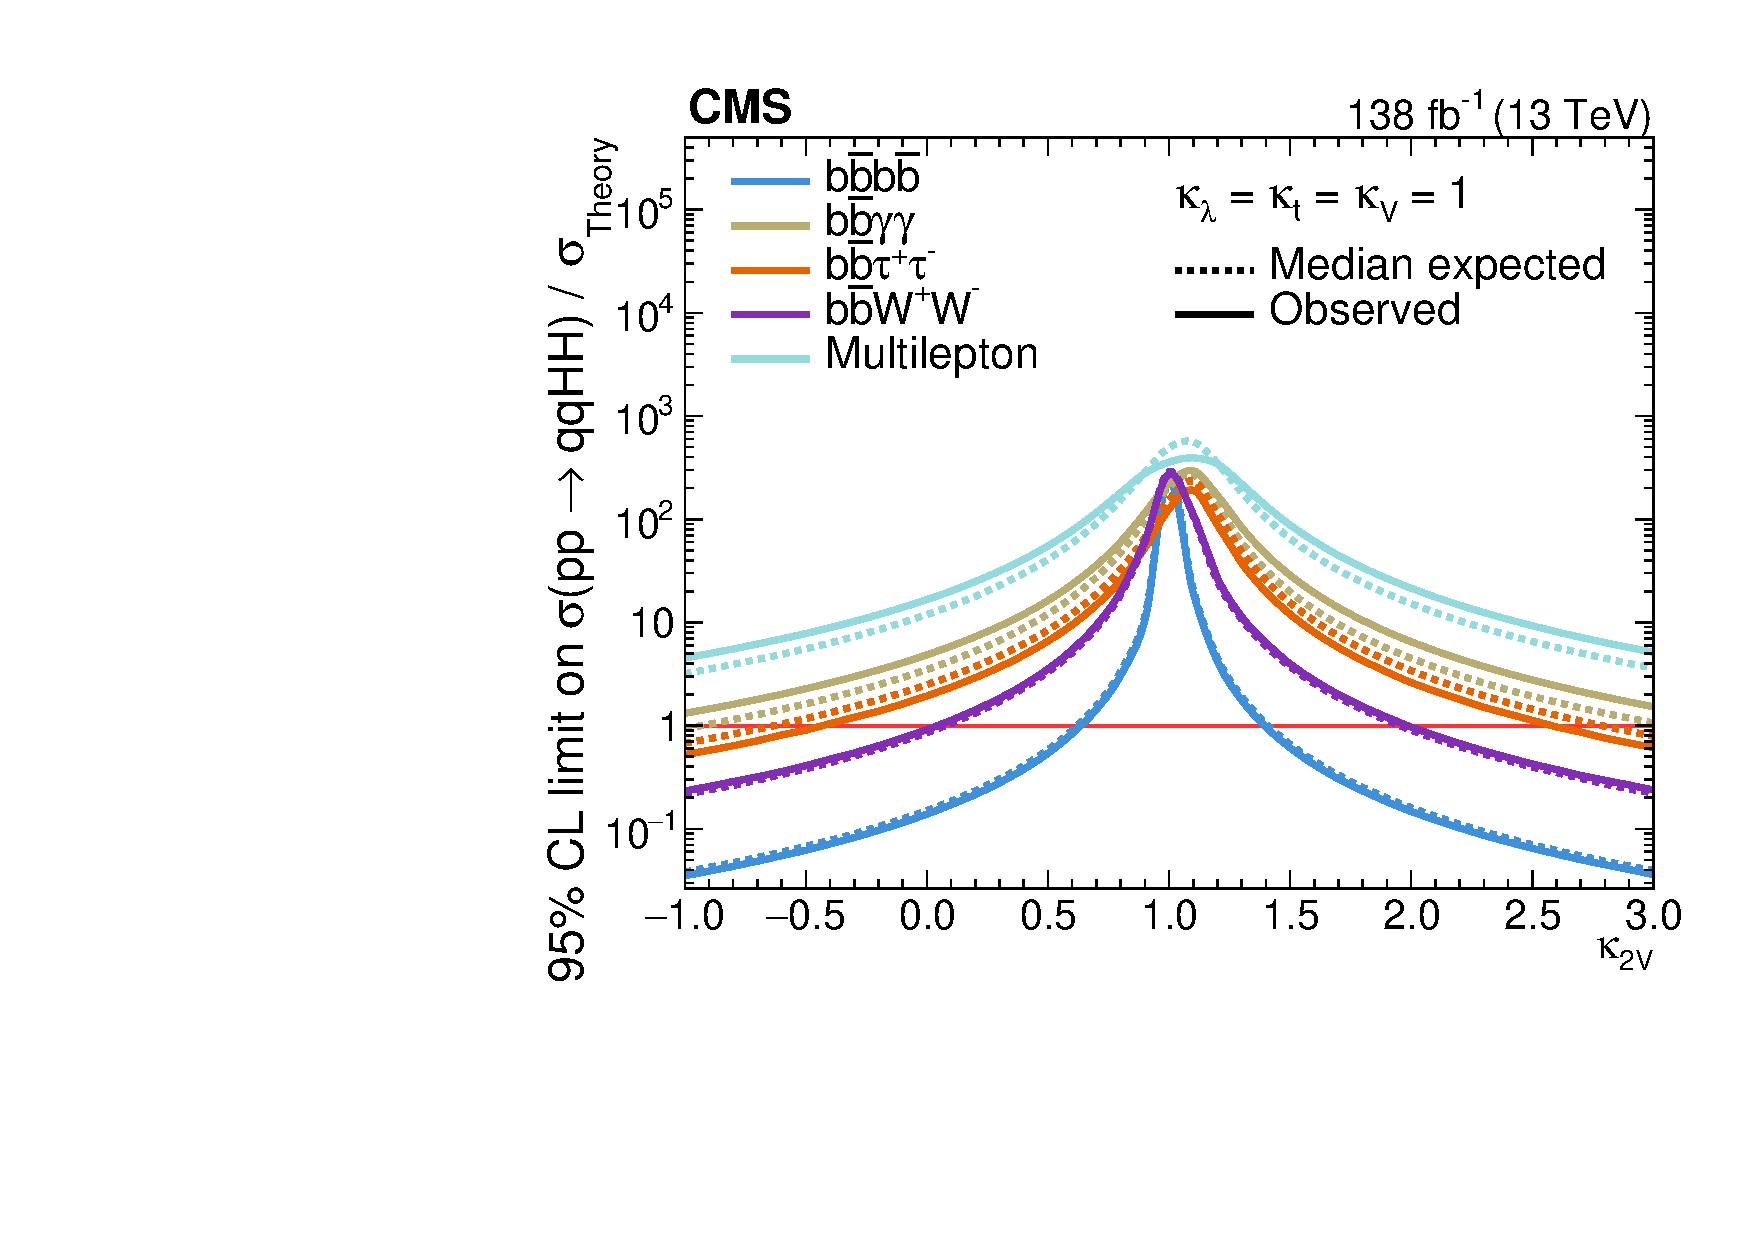
\includegraphics[width=0.49\textwidth]{figures/05-HH/CMS-results/C2V_limits_channels_rqqHH_paper.pdf}
    \caption[The expected and observed limits on the ratio of experimentally estimated production cross section and the theory expectation.]{The expected and observed limits on the ratio of experimentally estimated production cross section and the theory expectation for different values of \kapl (left) and \kapvv (right), reproduced from Ref.~\cite{CMS-PAS-HIG-20-011}.}
    \label{fig:05_hh_comb_kappa}
\end{figure}


In this dissertation, we present the first search for nonresonant \HH production in the \textit{all-hadronic \bbvv channel}, where one Higgs decays to two bottom quarks, while the other to two vector bosons (\VV) both decaying hadronically to the four quark (\qqqq) final state.
Both the \PW and \PZ bosons are considered for the latter decay and collectively referred to as \PV bosons.
The branching fractions for the \bbbar and \VV decays are $0.58$ and $0.25$ respectively, for a total branching fraction $\mathcal{B}(\HHbbVV) = 2  \cdot0.58\cdot 0.25 = 0.29$, which is the second-highest, behind only \bbbb.
The all-hadronic final state in particular has a branching fraction of $0.13$.
The analysis targets the boosted regime, which, as discussed above, has the two-fold advantage of 1) increasing sensitivity to \kapvv deviations and 2) exponentially reducing the dominant QCD multijet background.



\subsection{BSM \texorpdfstring{\XHY}{X→HY} production}
\label{sec:05_bsmxhy}

\begin{figure}[htb] %[ht]
    \centering
    % \captionsetup{justification=centering}
    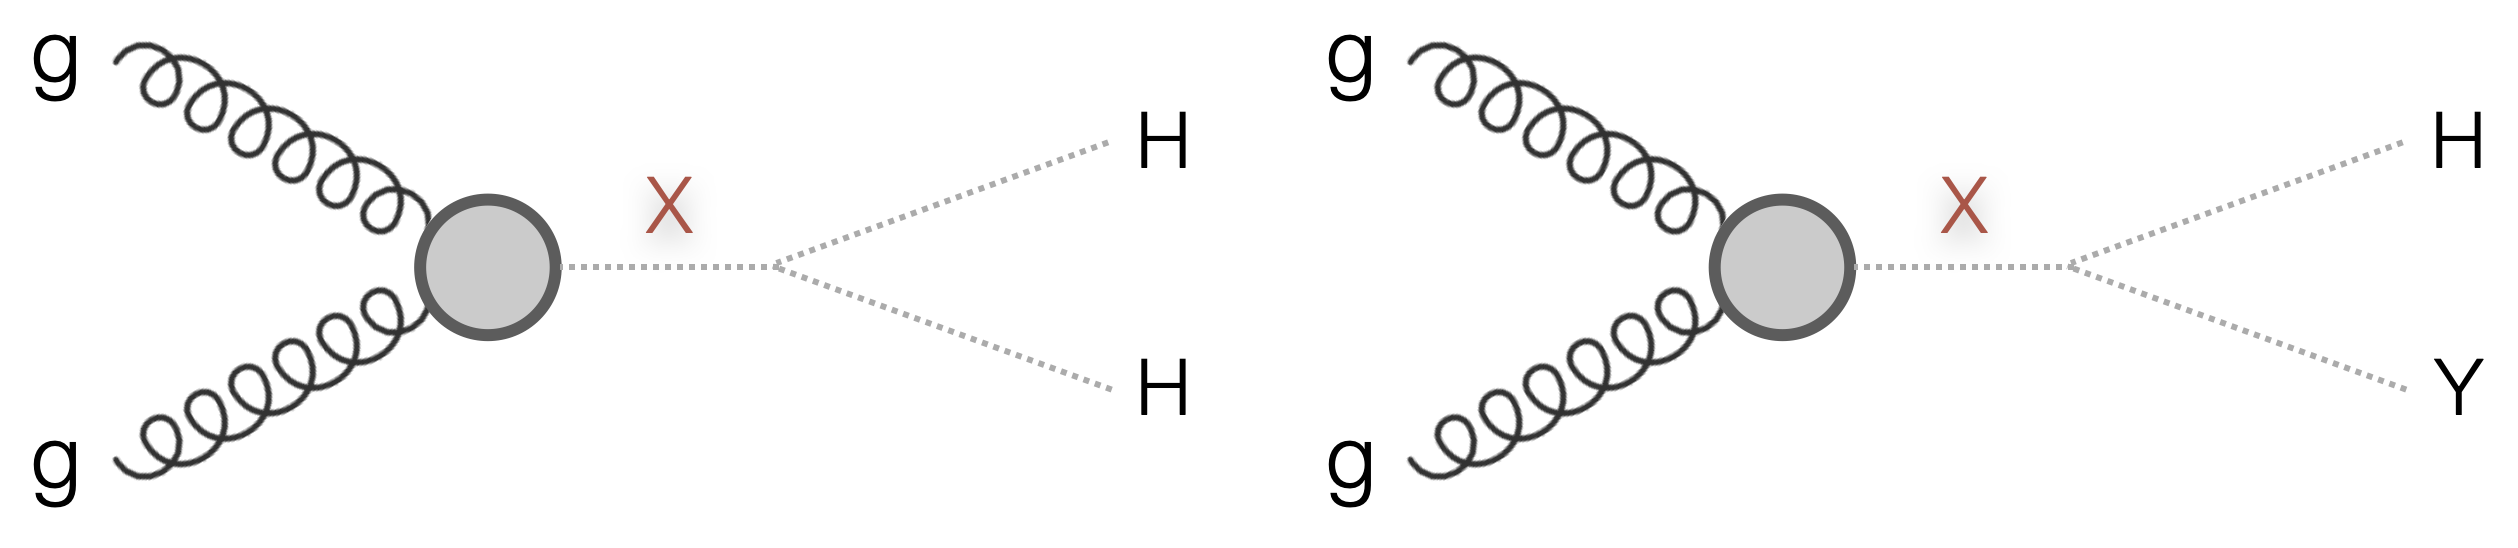
\includegraphics[width=\textwidth]{figures/05-HH/production/xhy.png}
    \caption{\XHY production in the symmetric (left) and asymmetric (right) cases.}
    \label{fig:05_xhy_production}
\end{figure}

Many theoretical models predict a richer scalar sector than that in the SM to address aesthetic and observational inconsistencies with the SM, such as the Higgs mass hierarchy problem and the baryon asymmetry discussed above.
These include two-Higgs doublet models (2HDM)~\cite{Branco:2011iw} that add an additional scalar doublet to the SM, such as the minimal supersymmetric extension of the SM (MSSM)~\cite{Craig:2013hca}, which predicts two neutral CP-even scalars (\PH, \Ph), one neutral CP-odd scalar (\PA), and two charged scalars ($\PH^\pm$), where one of the neutral CP-even scalars may be the discovered SM Higgs \PHsm.
The next-to-minimal supersymmetric extension of the SM (NMSSM)~\cite{Domingo:2022kfm} adds to this a complex scalar singlet, predicting two more CP-even ($\Ph_{\mathrm{s}}$) and CP-odd ($\Pa_{\mathrm{s}}$) neutral scalars.
Finally, the two-real-singlet-model (TRSM) predicts two additional CP-even scalar fields.
Depending on the kinematics, all these models allow for cascade decays of a heavier scalar to symmetric and asymmetric lighter scalars, such as $\PH\to\PHsm\PHsm$ and $\PH\to\Ph\PHsm$, respectively, as shown in Figure~\ref{fig:05_xhy_production}.

We search for this broad class of signals, looking for generic decays of the form \XHY, where \PX is the heavier and \PY the lighter scalar resonance, with \PH decaying to \bbbar and \PY to \VVq.
Many models, such as the TRSM, predict branching ratios for the lighter scalar similar to or the same as the SM Higgs.
In this case, the \VV decay modes are dominant for $\my > 140\GeV$ (Figure~\ref{fig:01_sm_higgs_hbrs}) and, hence, the \hbb and \yvv will be the dominant final states for the \XHY signal.
Thus, the \bbvv channel represents the highest BF in these models.

There are several published and ongoing CMS searches for \XHY production in a variety of regimes and final states with the Run 2 dataset, such as the boosted~\cite{BoostedXHY4b} \bbbb final state, the symmetric-only $\bbbar\PW\PW$ semi-leptonic final state~\cite{CMS:2024rgy}, the resolved $\bbbar\PGg\PGg$~\cite{CMS:2023boe}, and the resolved $\bbbar\PGt\PGt$~\cite{CMS:2021yci} final state.
This dissertation presents the first search in the \bbvv all-hadronic state, and the first in the \bbvv state for the asymmetric case, representing a significant increase in the covered phase space for \XHY searches.

The search comprises two distinct topologies depending on the ratio of the \PX and \PY masses: a highly-boosted fully-merged \yvv topology for $\mx \gg \my$, with both \VV bosons' decay products highly collimated into a single wide-radius jet; and a relatively less-boosted semi-merged topology, where the \VV bosons are well separated and each \vqq decay is reconstructed as its own wide-radius jet.
These two phases are illustrated in Figure~\ref{fig:05_xhy_fraction_3q4q}, showing the fraction of \yvv jets containing three or four generator-level quarks as a function of the \PX and \PY boson masses, with the transition occurring around $\mx \approx 10\my$.
This dissertation focuses on a search for the fully-merged topology only, i.e. for $\mx \gtrsim 10\my$, and is complementary to an ongoing CMS search in the semi-merged topology.
Thus, in terms of the analysis strategy and techniques, this search is similar to the boosted nonresonant \HH search in that they both target highly-boosted Higgs boson decays with single wide-radius jets for both \PH or \PY bosons.

\begin{figure}[htb] %[ht]
    \centering
    % \captionsetup{justification=centering}
    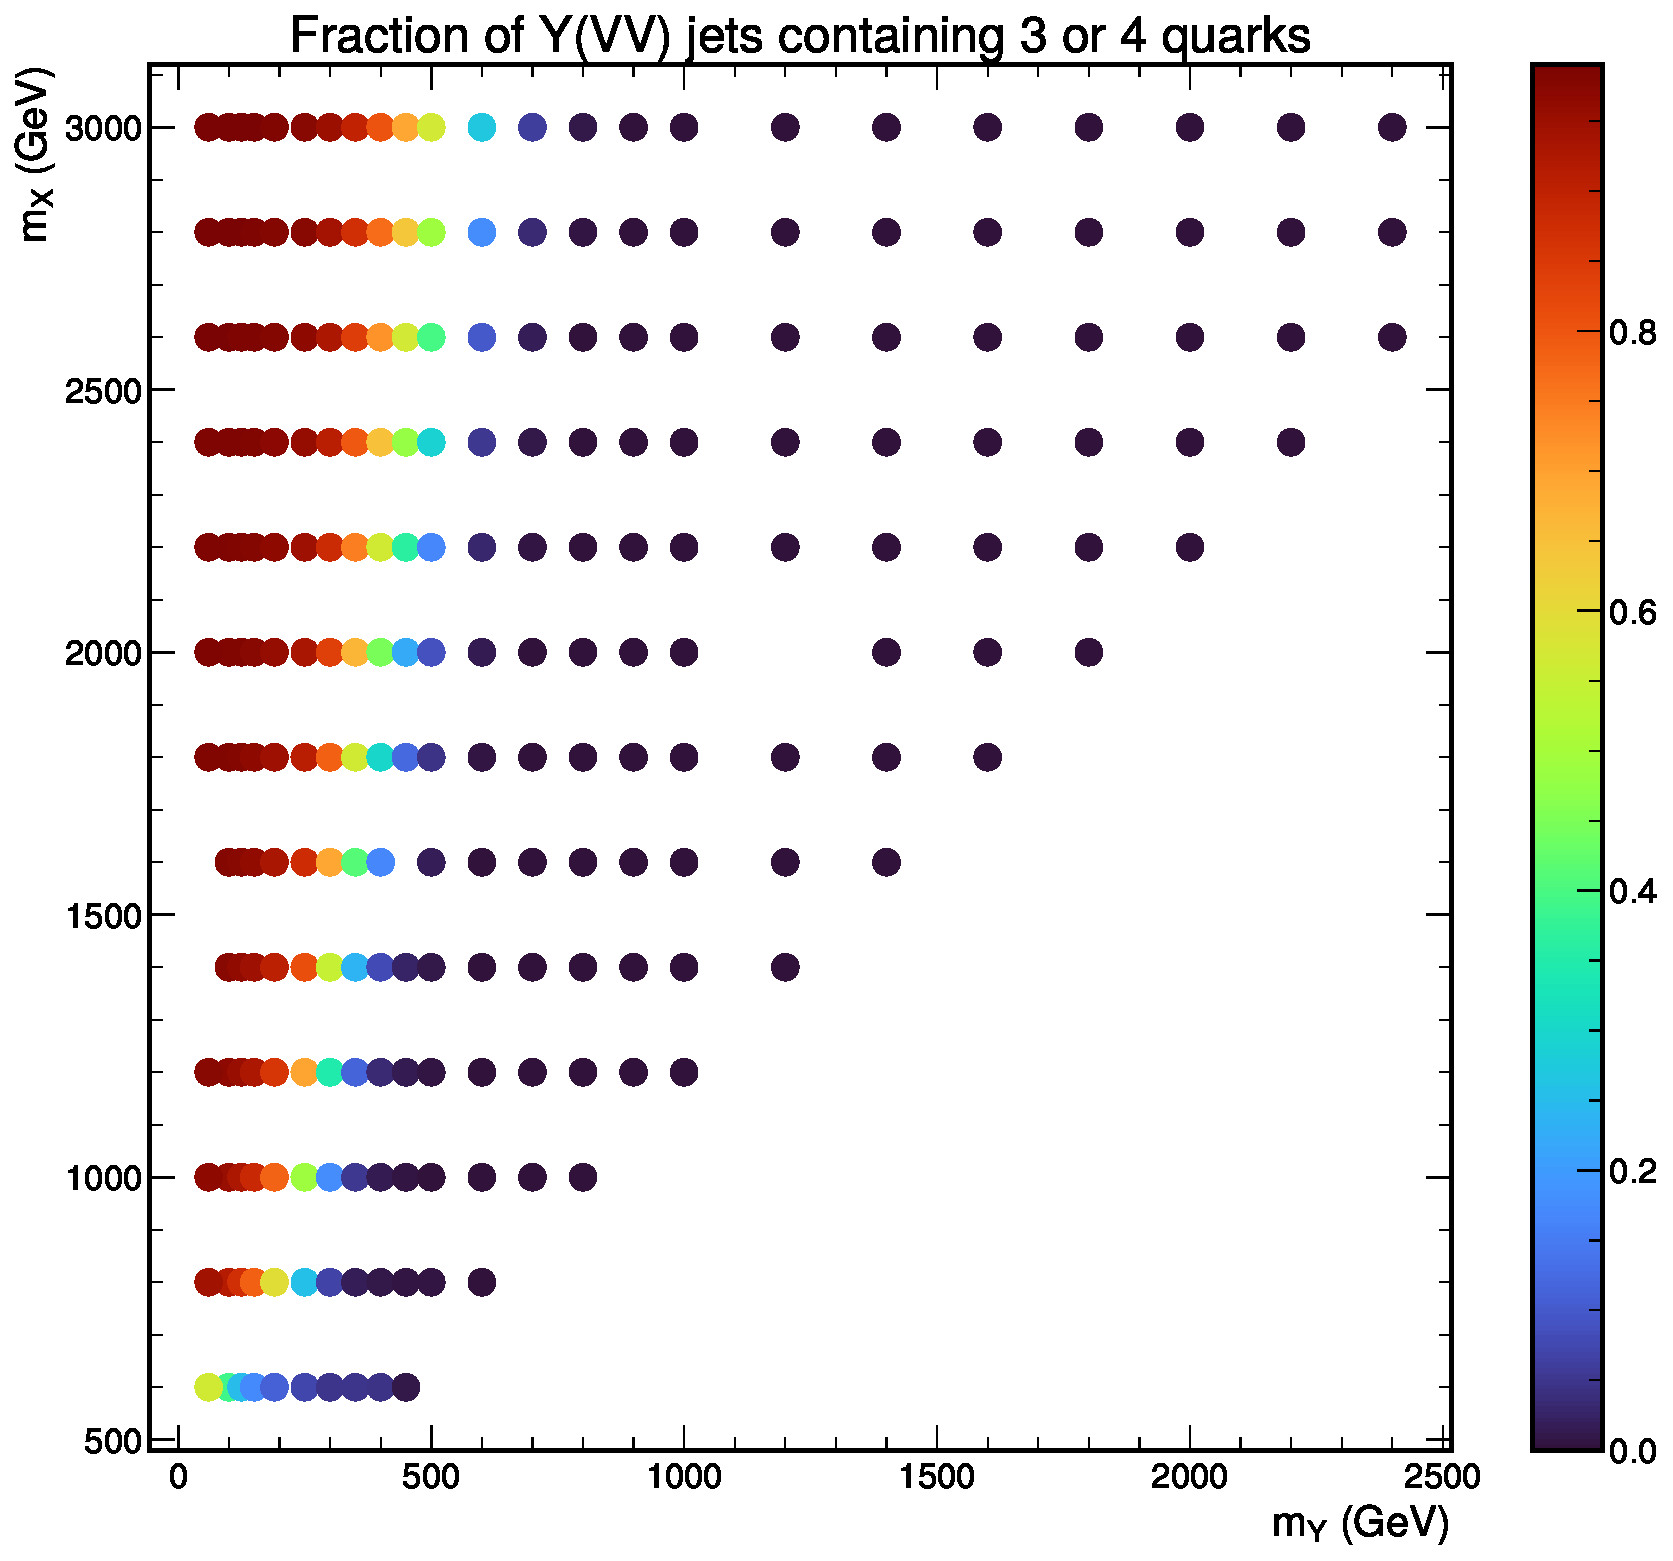
\includegraphics[width=0.8\textwidth]{figures/05-HH/production/fraction_3q4q.pdf}
    \caption{The fraction of \yvv jets containing three or four generator-level quarks for the resonant \XHYbbVV signal as a function of the \PX and \PY boson masses.}
    \label{fig:05_xhy_fraction_3q4q}
\end{figure}


% As shown in Figure~\ref{fig:01_sm_higgs_production}, both couplings can be accessed at the LHC exclusively through Higgs pair production.
% This dissertation describes one such measurement by the CMS experiment in the \bbvv channel, which is particularly sensitive to BSM deviations of the \HHVV coupling.
% It also presents a search for a new heavy resonance decaying to two Higgs bosons in the same channel, as predicted by many BSM theories described in Chapter~\ref{sec:05_bsmxhy}.


\subsubsection{Acknowledgements}

Chapters~\ref{sec:05_smhh} and~\ref{sec:05_bsmxhy} are in part, currently being prepared for the publication of the material by the CMS collaboration.
The dissertation author was the primary investigator and author of these papers.


% \section{Beyond the Standard Model}

% \subsection{Gravity}

%  - Gravity not a renormalizable QFT, can be thought of as an EFT in powers of (E/Mpl), so will never see the effect \\
%  - Experimentally, almost no consequence, but still fun to think about (although the 15 orders of magnitude gap makes you wonder if we are like the Greeks ``reasoning'' about atoms) \\
%  - String theory --- strings instead of particles, graviton arises, benefits: reproduces GR, SM etc. in the low-energy limit, but lots of unsolved problems \\
%  - Loop quantum gravity --- quantize space-time, only 4D, but so far does not reproduce our theories, interesting cosmological tests (constraint on spacetime quantization) \\
%  - Asymptotic safety --- Don't need gravity to be renormalizable, as long as the coupling constants have UV-safe fixed points (?), progress recently (see Weinberg 2009 lecture on motivation) \\


% \subsection{Grand unification}

%  - ``Zoo'' of particle representations can all be unified into two representations of a larger group SU(5), or even just a single huge representation of SO(10) (similar to two SU(2)'s embedded into SO(3, 1) or SO(4)) \\
%  - Very aesthetically pleasing, but moreover, lots of physical insights: charge quantization, proton charge = electron charge, \\
%  - SO(10) only: anti- / righthanded-neutrino, all fermions are encoded in ``five-bit strings'' (Zee) (although this predicts as-yet-unobserved fermions) \\
%  - Can keep adding bits / increasing the group size to include the different generations as well \\

%  - Similar to theories of quantum gravity, the GUT scale is so high that any effects will not be observed within our lifetimes sadly \\
%  - e.g. proton decay

% \subsection{Dark energy}

%  - Experimental evidence \\
%  - Higgs seesaw mechanism \\

% \subsection{Neutrino masses}

%  - Experimental evidence \\
%  - Seesaw mechanism \\

% \subsection{Dark matter}

%  - Experimental evidence \\
%  - WIMP, axion, sterile neutrinos, etc. \\
%  - Connections to Higgs \\

% \subsection{Baryon asymmetry}

%  - Sakharov conditions \\
%  - Relation to Higgs \\

% \subsection{Hierarchy problem}

%  - Is it a problem? \\
%  - Solutions \\

% \subsection{The SM as an effective field theory}

% HH EFT \\



% \section{Summary}
